% master.tex : master file for the project
% ------------------------------------------------------------------------------
% This is the main file in the project, which collects the contents from all the
% input files (text, images, literature databases, etc.).

% The 'book' class is a document class with many flexible options.
% See https://tex.stackexchange.com/a/36989/118167
\documentclass[11pt,a4paper,twoside,openright,english]{book}

% Some top level variables that are used to automatically input title, authors,
% etc. in the title page and front page.
\def \projecttitle       {Project Main Title}
\def \projectsubtitle    {Project Subtitle}
\def \projecttheme       {Project Theme}
\def \projectdegree      {Mathematics}  % or Mathematics-Economics/Technology
\def \projectperiod      {Spring Semester 2025}
\def \projectnumber      {P8}
\def \projectgroup       {MO8-05}
\def \projectauthors     {
  Project Author 1\\
  Project Author 2\\
  Project Author 3\\
  Project Author 4
  % ...
}
\def \projectsupervisors {
  Jan-Otto Hooghoudt\\
  Mikkel Meyer Andersen
  % ...
}

% The preamble, i.e. all the settings and commands that go before actual
% document contents, in this template is handled in the single file aaumath.sty,
% which defines a package that can be loaded here with \usepackage.
\usepackage{aaumath}

% All contents of the document go between the \begin and \end commands for the
% 'document' environment.
\begin{document}

% The front matter is not counted in the numbered pages and are instead numbered
% with roman numerals. This consists of, for example, the front page, title
% page, preface, and table of contents.
\frontmatter
% incl/misc/frontpage.tex : document front page
% ------------------------------------------------------------------------------


\backgroundsetup{
  scale = 1,
  angle=0,
  opacity=1,
  contents = {
    
\includegraphics[width=\paperwidth,height=\paperheight]{fig/img/aau/waves.pdf}
  }
}
\BgThispage
\pdfbookmark[0]{Front page}{frontpage}
\begin{titlepage}
  \centering
  \phantom{}
  \vspace{2cm}

  % AAU badge
  \begin{minipage}[c]{0.2\paperwidth}
    \centering
    \makebox[0pt]{
      % fig/tikz/aau-badge.tex : AAU logo badge for the front page
% ------------------------------------------------------------------------------

\begin{tikzpicture}
  % Draw white circle and add the transparent blue logo on top
  \node[circle,color=white,fill=white,minimum size=1.175\textwidth] at (0,0) {};
  \node at (0,0) {
\includegraphics[width=\textwidth]{fig/img/aau/logo-circle.pdf}};
\end{tikzpicture}

    }
  \end{minipage}

  % Main contents
  \vspace{4cm}
  {\fontfamily{bch}\selectfont
    \fboxsep0pt\colorbox{white}{
      \begin{minipage}{\textwidth}
        \centering
        \color{AAUblue1}

        \vspace{2em}
        {\Huge\bfseries\projecttitle}

        {\Large\bfseries\projectsubtitle}

        \bigskip
        \parbox{\textwidth}{\centering\large\projectauthors}

        \bigskip
        {\bfseries\large{\projectnumber} Project, Group \projectgroup, \projectdegree}
        \vspace{2em}
      \end{minipage}
    }
  }

\end{titlepage}

% incl/misc/titlepage.tex : project title page
% ------------------------------------------------------------------------------
% The title page is generated by the command \aautitlepage, which is defined in
% /incl/pre/ext/aautitlepage.sty


\pdfbookmark[0]{Title page}{titlepage}
\aautitlepage{
  \projectinfo{
    \projecttitle
  }{
    \projecttheme
  }{
    \projectperiod
  }{
    Group \projectgroup
  }{
    \parbox[t]{\textwidth}{\projectauthors}
  }{
    \parbox[t]{\textwidth}{\projectsupervisors}
  }{
    \today
  }
}{
  \textbf{Dept. of Mathematical Sciences}\\
  Thomas Manns Vej 23\\
  DK-9220 Aalborg\\
  \href{http://math.aau.dk}{http://math.aau.dk}
}{
  % incl/misc/abstract.tex : project abstract
% ------------------------------------------------------------------------------
% The abstract is a short summary of the document, displayed on the title page

}

% incl/misc/contents.tex :
% ------------------------------------------------------------------------------

\pdfbookmark[0]{Contents}{contents}

% The settings in this file are grouped so they only apply here
\begingroup

% Temporarily disable twoside layout to avoid blank pages in this section
\makeatletter
\@twosidefalse
\makeatother

% Put table of contents on its own page (best for a TOC that fits on one page)
\tableofcontents
\clearpage

% Put the lists on subsequent pages without page breaks
% \let\clearpage\relax
% \listoffigures
% \listoftables
% \listofalgorithms
% \lstlistoflistings

\endgroup


% The main matter is were the bulk of your work goes. Pages and headings have
% arabic numbers.
\mainmatter

% Input files should be partitioned such that each file corresponds to one
% chapter. The \include command forces a page break and inserts the contents of
% the input file.

\chapter{Pharmacometrics}

Pharmacokinetics (PK) is the study of how the body processes a drug. The overall process, from drug administration to drug elimination, can be divided into four phases: absorption, distribution, metabolism, and excretion. These four phases, elaborated in Section \ref{Sec: ADME and PK-parameters}, are often referred to by their acronym ADME. The overall PK process is typically modeled by the aid of compartment models, elaborated in Section \ref{sec: compartment models}, accompanied by a number of PK parameters with a clear physiological interpretation in relation to drug absorption, distribution and elimination. 

Pharmacodynamics (PD), elaborated in Section \ref{sec: Pharmacodynamics}, is the study of the effects of a drug on the body.  In Section \ref{sec: PK/PD-modelling} a PK/PD approach to model delayed effect is introduced.

\section{Pharmacokinetics: ADME} \label{Sec: ADME and PK-parameters}

% \subsection*{Absorption}
The \textbf{absorption} phase describes the process of the drug being absorbed into the systemic circulation after drug administration. The three main routes of drug administration are orally, i.e. by tablet, subcutaneous (SQ), i.e. by injection, or intravascular (IV), i.e. directly into vein. The drug absorption process is typically described through the absorption rate parameter $k_a$ ([1/hour]).

Another important parameter in relation to drug absorption is the bioavailability, $F \in [0,1]$, which denotes the fraction of the administered drug dose, that reaches the systemic circulation. The mass of drug delivered to the systemic circulation is then the product of the given dose, $D$, and $F$, i.e. $F \cdot D$.

Drugs administered IV require no absorption phase as the drug is delivered directly into the systemic circulation, with a bioavailability of $F=1$. Drugs administered extravascularly (EV), i.e. not injected directly into the systemic circulation, require an absorption phase, resulting in a bioavailability of $F <1$.

% \subsection*{Distribution}
The \textbf{distribution} of drug into various tissues of the body (e.g. fat, muscle, and brain tissue) occurs when the drug is absorbed into the systemic circulation. The distribution of drug is modelled in a compartment model setup with exchange rate parameters describing the exchange of drug between compartments. In two-compartment models (introduced in Section \ref{sec: compartment models}), the exchange rate parameters are $k_{12}$ and $k_{21}$ ([1/hour]), which represent the rates of drug exchange between the central and peripheral compartments, respectively. 

The distribution of a drug depends on its biochemical properties as well as the physiology of the individual taking it. In this phase, the drug reaches its place of action and the aim is to achieve the desired drug concentration. 

Drug concentration is measured as the concentration of drug in the plasma, $C$ ([mg/L]), regardless of the place of action of the drug. The primary parameter describing drug distribution is the volume of distribution, $V$ ([L]), that is the total volume a drug has to distribute uniformly into to reach a given concentration in the plasma. Drugs with larger $V$ are thereby exchanged more to other tissues than drugs with lower $V$. The relation between the concentration of drug in the plasma and the volume of distribution is
\begin{align} \label{eq: Concentration}
    C = \frac{A}{V},
\end{align}
where $A$ ([mg]) is the amount of drug. 


% \subsection*{Metabolism}
The \textbf{metabolism} phase, reached after the drug has been absorbed and distributed throughout the body, refers to the process in which the body chemically alters the molecules of a drug, which creates new compounds called metabolites. 
The majority of metabolism occurs in the liver, but it can occur in many areas of the body  including the gastrointestinal tract, kidneys, and plasma.

The metabolism is a part of the elimination of the drug, i.e. the process of removing the administered drug from the body. Any drug that is not eliminated from the body through metabolism is instead eliminated by excretion.


% \subsection*{Excretion}
Drug \textbf{excretion} is the removal of the administered drug and its metabolites from the body. Drugs can be excreted by several routes including the liver, lungs, gastrointestinal tract, and skin, however most drugs are excreted through the kidneys with urine. 

The primary PK parameter describing the elimination of the drug through metabolism and excretion is clearance, $CL$ ([L/hour]), which states the volume of plasma cleared of drug within a certain time interval, thereby representing the efficiency of drug elimination. 

The first order elimination rate constant, $k_e$ ([1/hour]), is defined by the clearance and volume of distribution as 
\begin{align} \label{eq: elimination rate constant}
    k_e = \frac{CL}{V}.
\end{align}
That is, $k_e$ is the fraction of volume cleaned in a certain time interval, typically per hour.


\section{Compartment Models} \label{sec: compartment models}

Compartment models are a central tool in describing the overall drug processing in the body. They consist of a central compartment, zero or more peripheral compartments, and, if the route of administration is EV, a depot (absorption site). The central compartment represents the plasma and highly perfused tissues (such as lungs, liver and kidneys), where drug concentration is measured. If the drug cannot be reasonably assumed to distribute instantly and homogeneously through the entire system after absorption, peripheral compartments can be included to represent poorly perfused tissues (such as muscle and skin), where the drug distributes to and from the central compartment. 

% Peripheral compartments can be included if the drug cannot be reasonably assumed to distribute instantly and homogeneously through the entire system after absorption.

% In Figure \ref{fig: One-compartment model}, a one-compartment model with depot is schematically depicted. In a one-compartment model, the body is be represented as a single compartment in which the distribution of the drug is instantaneous and homogeneous through the entire system after absorption. This is, however, often an extreme simplification in practice \citep[p. 174]{Talevi2024}.

% In Figure \ref{fig: Two-compartment model}, a two-compartment model without depot is schematically depicted. In a two-compartment model, the body is represented with a central compartment consisting of the plasma and highly perfused tissues (such as lungs, liver and kidneys), and a peripheral compartment representing poorly perfused tissues (such as muscle and skin). In the two-compartment model, the drug is thereby not assumed to be evenly distributed throughout the body, but instead distributed between these two different compartments. This is the idea of compartmental modeling with two or more compartments; grouping together tissues with similar blood flow rates to allow for the parameters to be more accurately estimated \citep{chen2024pharmacokinetics}.

% ASSUMPTIONS ON THE MODEL %
The one-compartment model only contains a central compartment, while the two-compartment model also contains a peripheral compartment.
In both models, elimination only occurs from the central compartment and follows first order kinetics, meaning the rate of elimination is proportional to the amount of drug left in the central compartment. With EV administration, a depot is included in the model, and absorption into the central compartment follows first order kinetics, meaning that the rate of absorption is proportional to the amount of drug left in the depot. 
In the two-compartment model, the drug initially enters the central compartment. Furthermore, the distribution of drug from the central compartment to the peripheral compartment, and vice versa, follows first order kinetics. 

% WHAT TO SPECIFY 
Many scenarios can be represented using compartmental modeling, provided that the following are specified: 1) number of compartments (one, two, or more), 2) route of administration (IV, oral, SQ, etc.), implying whether a depot is included or not, and 3) dosage regimen (single/multiple dosage (see Appendix \ref{app: other dosage regimen}) etc.).


% MODELS IN THIS REPORT 
The models of consideration are the one-compartment model with and without depot, and the two-compartment model with depot, all with dosage regimen being a single dose. The compartment model structure is formalised by deriving expressions for the amount of drug in the central compartment as a function of time using ordinary differential equations (ODEs). 


% Drug absorption either follows zero order kinetics (meaning the rate of absorption is constant, e.g. constant rate IV infusion) or first order kinetics (e.g. oral administration).


% Many different scenarios can be modelled using compartment models. To construct the correct model for a given scenario, one should always specify
% \begin{enumerate}[label=\arabic*)]
%     \item assumed number of compartments (one, two, or more), \label{item: ass number of comp}
%     \item route of administration (IV, oral, SQ, etc.), and \label{item: route of adm}
%     \item dosage regimen (single dosage, constant rate infusion, multiple dosage, etc.).
% \end{enumerate}
\begin{figure}[h]
    \centering
    \begin{subfigure}[b]{0.48\textwidth}
    \centering
        \begin{tikzpicture}[node distance=1cm, >=Stealth, thick, scale=1, transform shape] % Smaller figure
      % Absorption Model
      \node[draw, fill=white!10, minimum width=2.5cm, minimum height=1.2cm, align=center] (absorption) {Depot};
      \node[draw, fill=gray!10, minimum width=2.5cm, minimum height=1.2cm, right=1.5cm of absorption, align=center] (central) {Central};

      % Arrows for Absorption Model
      \node[above=0.6cm of absorption] (labelFA) {$\ F \cdot D$}; % Moved label higher
     \draw[<-] (absorption.north) ++(0,-0.36) -- ++(0,1);
      \draw[->] (absorption.east) -- (central.west) node[midway, above] {$k_a$};
      \draw[->] (central.south) -- ++(0,-1) node[midway, right] {$k_e$};
    \end{tikzpicture}
        \caption{One-compartment model with depot (EV administration).}
        \label{fig: One-compartment model}
    \end{subfigure}
    \hfill
    \begin{subfigure}[b]{0.48\textwidth}
        \centering
\begin{tikzpicture}[node distance=1cm, >=Stealth, thick, scale=1, transform shape] 
    % Two-Compartment Model
    \node[draw, fill=gray!10, minimum width=2.5cm, minimum height=1.2cm, align=center] (central2) {Central};
    \node[above=0.6cm of central2] (labelA0) {$D$}; % Moved label higher
     \draw[<-] (central2.north) ++(0,-0.36) -- ++(0,1);
    \node[draw, fill=gray!10, minimum width=2.5cm, minimum height=1.2cm, right=1.5cm of central2, align=center] (peripheral) {Peripheral};

    % First Arrow (top)
    \draw[->] (central2.east) ++(0,0.1) -- ++(1.5,0) node[midway, above] {$k_{12}$};
    
    % Second Arrow (bottom) with vertical shift
    \draw[<-] (central2.east) ++(0, -0.1) -- ++(1.5,0) node[midway, below] {$k_{21}$};
    
    % Vertical Arrow
    \draw[->] (central2.south) -- ++(0,-1) node[midway, right] {$k_e$};
\end{tikzpicture}
        \caption{Two-compartment model without depot (IV administration).}
        \label{fig: Two-compartment model}
    \end{subfigure}
    \caption{Compartment models illustrating drug movement in the body. The grey boxes represent compartments; each representing a homogeneous system in which the drug is assumed to be uniformly distributed. The white box illustrates a depot that drugs administrated EV have to pass through to reach the systemic circulation. The arrows from $F \cdot D$ and $D$ indicate the amount of drug that reaches systemic circulation, while the arrows between the compartments represent drug transitions. The transitions are described by the rate constants $k_a, k_e, k_{12}$ and $k_{21}$.}
    \label{fig: Compartment models}
\end{figure}

\subsection{One-compartment model}
The one-compartment model is depicted in Figure \ref{fig: One-compartment model} without the depot. The mass balance equation for the central compartment is given by the ODE
\begin{align} \label{eq: first order kinetic of amount in one com without abs}
    \Dif{A_{c}(t)} = - k_e * A_{c}(t),
\end{align}
where $A_{c}(t)$ is the amount of drug in the central compartment at time $t$. The solution to \eqref{eq: first order kinetic of amount in one com without abs} is given by
\begin{align} \label{eq: sol to first order kinetic of amount in one com without abs}
    A_{c}(t) = D * \exp(-k_e * t). 
\end{align} 

\subsection{One-compartment model with depot}
The one-compartment model with depot is depicted in Figure \ref{fig: One-compartment model}. The mass balance equation for the central compartment is given by the system of two ODEs
\begin{align} \label{eq: first order kinetic of amount in central com with abs com}
    \Dif{A_{d}(t)}    &= - k_a * A_{d}(t) \nonumber\\
    \Dif{A_{c}(t)} &= k_a * A_{d}(t) - k_{e} * A_{c}(t),
\end{align}
where $A_{d}(t)$ is the amount of drug in the depot at time $t$.
% The first term on the right hand side represents the rate of drug absorbed by the central compartment, while the last term represents the rate of drug eliminated from the central compartment.
The solution to \eqref{eq: first order kinetic of amount in central com with abs com} is given by
\begin{align} \label{eq: sol to first order kinetic of amount in central com with abs com}
    A_{c}(t) = \frac{k_a F D}{k_a - k_e} \left( \exp(-k_e * t) - \exp(-k_a * t) \right).
\end{align}

\subsection{Two-compartment model with depot}
The two-compartment model with depot is depicted in Figure \ref{fig: Two-compartment model} with an added depot. The mass balance equations for the central and peripheral compartments are given by the system of three ODEs
\begin{align}
    \Dif{A_{d}(t)}    &= - k_a * A_{d}(t) \nonumber \\
    \Dif{A_{c}(t)}    &= k_a * A_{d}(t) + k_{21} * A_{p}(t) - k_{12} * A_{c}(t) - k_e * A_{c}(t), \label{eq: 2-comp central}\\
    \Dif{A_{p}(t)} &= k_{12} * A_{c}(t) - k_{21} * A_{p}(t),\nonumber
\end{align}
% \begin{align*}
%     \Dif{A_{c}(t)}    &= k_{21} * A_{p}(t) - k_{12} * A_{c}(t) - k_e * A_{c}(t),\\
%     \Dif{A_{p}(t)} &= k_{12} * A_{c}(t) - k_{21} * A_{p}(t),
% \end{align*}
where $A_p(t)$ is the amount of drug in the peripheral compartment at time $t$. The solution to \eqref{eq: 2-comp central} is given by
\begin{align*}
    A_{c}(t) = D  k_{a} \left( \frac{A e^{-\alpha t} \left( e^{(\alpha - k_{a})t} - 1 \right)}{\alpha - k_{a}} + \frac{B e^{-\beta t} \left( e^{(\beta - k_{a})t} - 1 \right)}{\beta - k_{a}} \right),
\end{align*}
where $A = \frac{\alpha - k_{21}}{\alpha - \beta}$, $B = \frac{k_{21} - \beta}{\alpha - \beta}$, $\alpha + \beta = k_{12} + k_{21} + k_{e}$ and $\alpha \beta = k_{21} * k_{e}$.


% \begin{align*}
%     A_{c}(t) = \psi * \exp(- \alpha t) + \gamma * \exp(- \beta t),
% \end{align*}
% where $\psi = \frac{D * (\alpha - K_{21})}{\alpha - \beta}$, $\gamma = \frac{D * (k_{21} - \beta)}{\alpha - \beta}$, $\alpha + \beta = k_{12} + k_{21} + k_{e}$ and $\alpha \beta = k_{21} * k_{e}$.


% \subsection{Formalizing Compartment Dynamics: Multiple scenarios}



% Consider the scenario of a one-compartment model with IV administration of a single dose $D$. This is equivalent with the model shown in Figure \ref{fig: One-compartment model}, without the absorption site, meaning that $D$ is injected directly to the central compartment. Assuming drug elimination follows first order kinetics, the rate of change in the central compartment, also known as the mass balance equation for the central compartment, is given by the differential equation
% \begin{align} \label{eq: first order kinetic of amount in one com without abs}
%     \Dif{A_{central}(t)} = - k_e * A_{central}(t),
% \end{align}
% where $A_{central}(t)$ denotes the amount of drug in the central compartment at time $t$, and $k_e$ denotes the elimination rate constant. The solution to \eqref{eq: first order kinetic of amount in one com without abs} is given by
% \begin{align} \label{eq: sol to first order kinetic of amount in one com without abs}
%     A_{central}(t) = D * \exp(-k_e * t). 
% \end{align} 

% Consider the scenario of a one-compartment model with EV administration of a single dose $D$, represented in Figure \ref{fig: One-compartment model}. Assuming drug absorption and elimination follows first order kinetics, the mass balance equation for the central compartment is given by 
% \begin{align} \label{eq: first order kinetic of amount in central com with abs com}
%     \Dif{A_{central}(t)} = K_a * A_{absorption}(t) - K_{e} * A_{central}(t),
% \end{align}
% where $A_{absorption}$ denotes the amount of drug at the absorption site and $K_a$ is the absorption rate constant. The first term on the right hand site represents the rate of drug absorbed by the central compartment, while the last term represents the rate of drug eliminated from the central compartment.
% The solution to \eqref{eq: first order kinetic of amount in central com with abs com} is given by
% \begin{align} \label{eq: sol to first order kinetic of amount in central com with abs com}
%     A_{central}(t) = \frac{K_a F D}{K_a - k_e} \left( \exp(-k_e * t) - \exp(-K_a * t) \right).
% \end{align}

% In some cases, a one-compartment model might be a too restrictive assumption. Therefore, consider a two-compartment model with IV administration of a single dose, represented in Figure \ref{fig: Two-compartment model}. Assuming the drug absorption, elimination, and distribution between the compartments follow first order kinetics, the mass balance equations for the two compartments constitute a system of two differential equations given by
% \begin{align*}
%     \Dif{A_{central}(t)}    &= K_{21} * A_{peripheral}(t) - K_{12} * A_{central}(t) - k_e * A_{central}(t),\\
%     \Dif{A_{peripheral}(t)} &= K_{12} * A_{central}(t) - K_{21} * A_{peripheral}(t),
% \end{align*}
% where $A_{peripheral}(t)$ denotes the amount of drug in the peripheral compartment, $K_{21}$ denotes the rate constant representing the flow of drug from the peripheral compartment to the central compartment, and $K_{12}$ denotes the rate constant representing the flow of drug from the central compartment to the peripheral compartment.
% Since the concentration of drug is measured in the plasma, only the solution for the central compartment is necessary. The solution is given by
% \begin{align*}
%     A_{central}(t) = \psi * \exp(- \alpha t) + \gamma * \exp(- \beta t),
% \end{align*}
% where $\psi = \frac{D * (\alpha - K_{21})}{\alpha - \beta}$, $\gamma = \frac{D * (K_{21} - \beta)}{\alpha - \beta}$, $\alpha + \beta = K_{12} + K_{21} + K_{e}$ and $\alpha \beta = K_{21} * K_{e}$.

% It is possible to consider other dosing regimens and more complex compartment structures to obtain more realistic models. Accurate models are, of course, desirable, but a simple one- or two-compartment model might be sufficient enough to obtain an acceptable PK profile, i.e. estimates of the PK parameters listed in Table \ref{tab: pharmacokinetic parameters summary}, of a drug.

% In practice, it is the concentration of the drug in the plasma, $C(t)$, that is measured. For this reason, it is necessary to represent the solutions in terms of concentration which is related to $A(t)$ by \eqref{eq: Concentration}.


\section{Pharmacodynamics} \label{sec: Pharmacodynamics}
The objective of pharmacodynamics (PD) is to model the effect of a drug. For a drug to produce an effect, the drug molecule has to interact with cells. The interaction occurs as a drug molecule attaches to a receptor. Each cell membrane is covered with receptors, where drug molecules can bind. Once a drug molecule binds to a receptor, that receptor becomes blocked, preventing other drug molecules from binding to it. The process of interaction can be described as
\begin{align} \label{eq: Reversible receptor}
    [M] + [R] & \overset{k_1}{\underset{k_{-1}}{\rightleftarrows}} [MR],
\end{align}
where, $[M]$ is the amount of unbounded drug molecules, $[R]$ is the unoccupied receptors, and $[MR]$ is the bound drug/receptor complex, being the association that occurs when a drug molecule binds to a receptor. The constant $k_1$ indicates the rate at which unbound receptors become occupied, and $k_{-1}$ represents the rate at which bound receptors revert to be unbounded. The relation $K_d = k_{-1}/k_1$ is the disassociation.
The rate of change in amount of bound receptor complexes is expressed as
\begin{align} \label{eq: steady state PD}
    \Dif{[MR]} = k_1 [R][M] - k_{-1}[MR],
\end{align}
where on the right hand side, the first term is the rate at which molecules bind to receptors, and the second term is the rate at which the receptors revert to be unbounded. 
The effect of a drug is quantified as 
\begin{align} 
    E &= \varphi[MR] \label{eq: effect formalisation}
\end{align}
as only a proportion, $\varphi \in [0, 1]$, of the complexes are active, i.e. yield an effect.
The maximal effect, $E_{max}$, is achieved when the total number of receptors, $[R_{tot}] = [R] + [MR]$, are occupied. Hence,
\begin{align}
    E_{\text{max}} = \varphi[R_{tot}]. \label{eq: effect formalisation2}
\end{align}

The PD parameters of interest are $E_{max}$ and $K_d$, hence the effect is rewritten as 
\begin{align}
    E = \frac{E_{\text{max}}[M]}{[M] + K_d}, \label{eq: effect with m and kd}
\end{align}
derived from \eqref{eq: steady state PD}, \eqref{eq: effect formalisation}, \eqref{eq: effect formalisation2}, and the expression for $R_{tot}$, see Appendix \ref{app: }.
The parameters are estimated using the Sigmoid $E_{\text{max}}$ model,
\begin{align}\label{eq: sigmoid emax}
    E(C) = E_0 + \frac{E_{\text{max}}C^n}{C^n+C_{50}^n}, 
\end{align}
which approximates \eqref{eq: effect with m and kd} with $C$ representing $[M]$ and $C_{50}$ representing $K_d$, while allowing a baseline effect, $E_0$. By definition, $C_{50}$ is the concentration at which the effect reaches $50\%$ of its maximal increase from baseline, i.e. $E(C_{50}) = E_0 + 1/2 E_{\text{max}}$. The parameter $n$ provides a further degree of flexibility.

\begin{figure}[H]
    \centering
    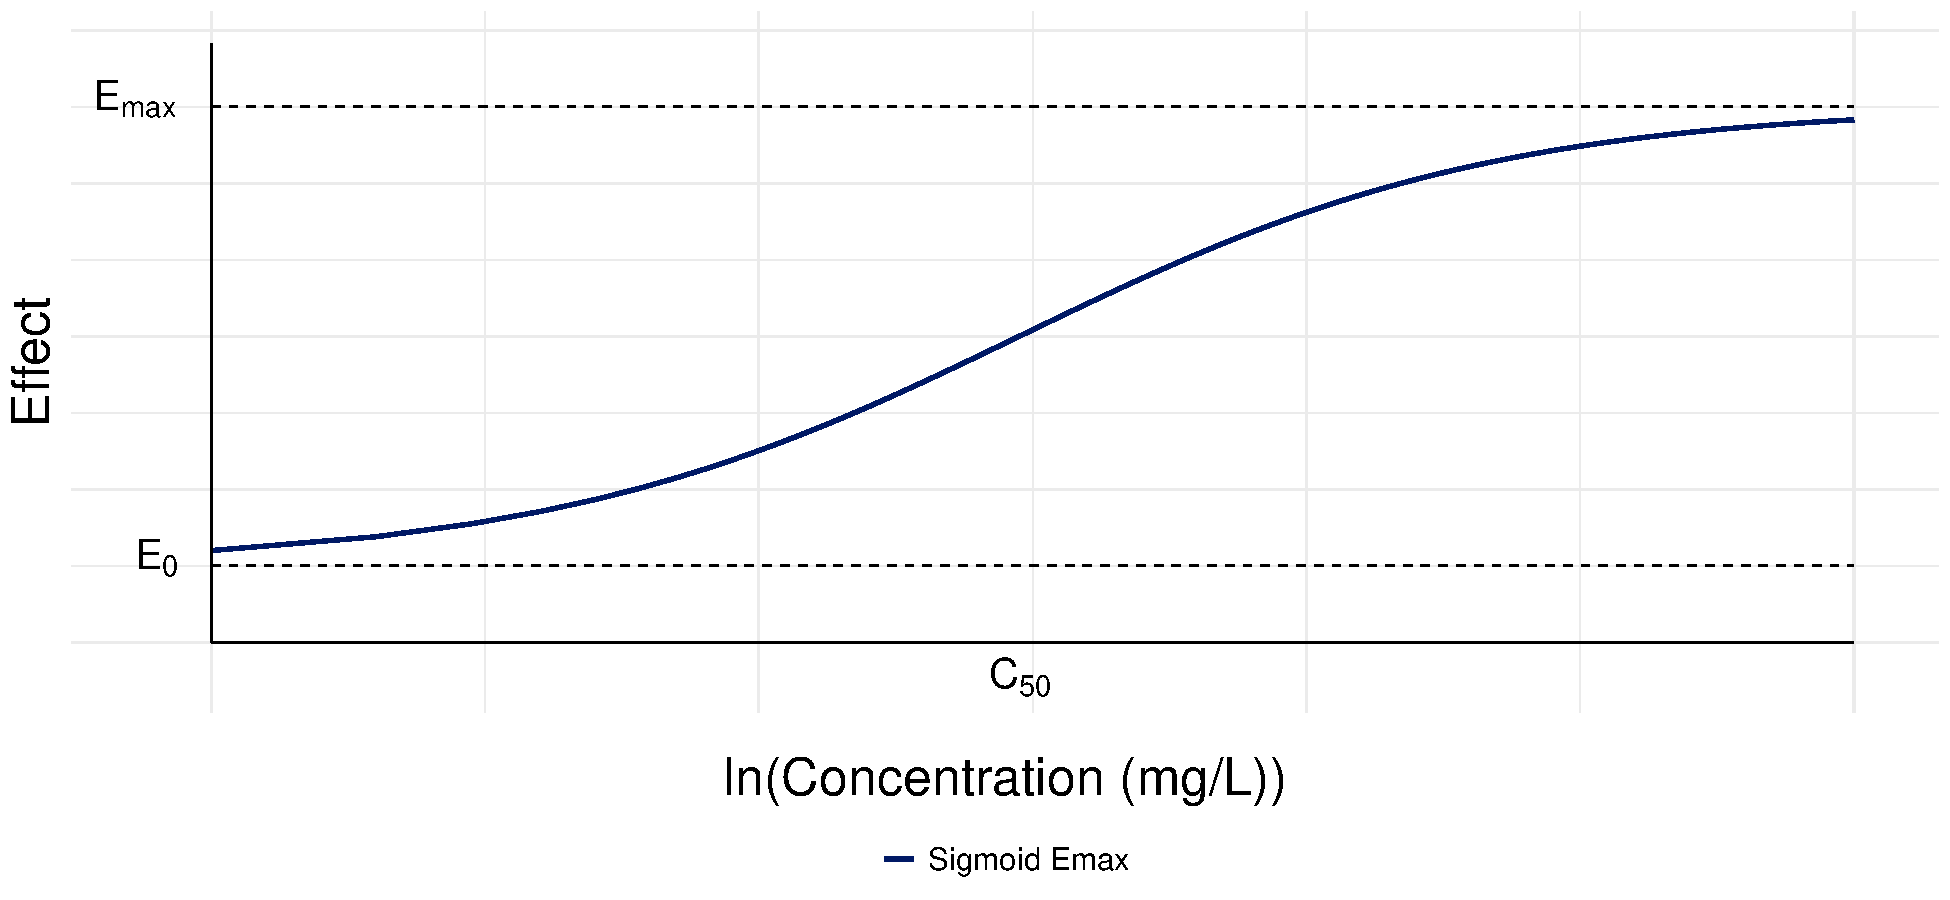
\includegraphics[width=0.9\linewidth]{fig/img/PD/ModelPlots.pdf}
    \caption{Example of $\ln(\text{Concentration})$ vs. PD-models.}
    \label{fig: Different PD-models}
\end{figure}

The effect may be delayed relative to the concentration level. The delay in effect can be modeled by including a hypothetical effect compartment, into the compartmental model used in PK. The effect compartment distributes a negligible amount of concentration from and to the central compartment, see Figure \ref{fig: One-compartment model with effect}, thus having no impact on the concentration within the central compartment.
\begin{figure}[H]
    \centering
    \begin{tikzpicture}[node distance=1cm, >=Stealth, thick, scale=1, transform shape] % Smaller figure
      % Absorption Model
      \node[draw, fill=white!10, minimum width=2.5cm, minimum height=1.2cm, align=center] (absorption) {Absorption};
      \node[draw, fill=gray!10, minimum width=2.5cm, minimum height=1.2cm, right=1.5cm of absorption, align=center] (central) {Central};
      \node[draw, fill=gray!15, minimum width=2.5cm, minimum height=1.2cm, above=1.5cm of central, align=center] (effect) {Effect};

      % Arrows for Absorption Model
      \node[above=0.6cm of absorption] (labelFA) {$\ F \cdot D$}; % Moved label higher
    \draw[<-] (absorption.north) ++(0,-0.36) -- ++(0,1);
    \draw[->] (absorption.east) -- (central.west) node[midway, above] {$k_a$};
    \draw[->] (central.south) -- ++(0,-1) node[midway, right] {$k_e$};

    \draw[dotted, ->] (central.north) ++(0.1,0) -- ++(0,1.5) node[midway, right] {$k_{e1}$};
    
    % Second Arrow (bottom) with vertical shift
    \draw[dotted, <-] (central.north) ++(-0.1, 0) -- ++(0,1.5) node[midway, left] {$k_{e0}$};


    \end{tikzpicture}
    \caption{One compartment model with absorption site and effect compartment.}
    \label{fig: One-compartment model with effect}
\end{figure}
The amount of drug in the effect compartment is described as
\begin{align} \label{eq: Concentration in effect compartment}
    \Dif{A_e} = k_{e1} * A_{\text{central}} - k_{e0} A_e,
\end{align}
where $A_e$ denotes the amount of drug in the effect compartment, $k_{e1}$ denotes the distribution of drug from the central compartment to the effect compartment, $k_{e0}$ denotes the distribution of drug from the effect compartment to the central compartment. The concentration of drug in the effect compartment is defined as
\begin{align*}
    C_e(t) = \frac{k_{e1} D}{V(k_{e1} - k_{e0})} \left( \exp(-k_{e0} * t) - \exp(-k_{e1} * t) \right).
\end{align*}
Drug concentration within the central compartment and effect estimated using the Sigmoid Emax model on the concentration in the effect compartment, is depicted in Figure \ref{fig: PKPDmodel}.
\begin{figure}[H]
    \centering
    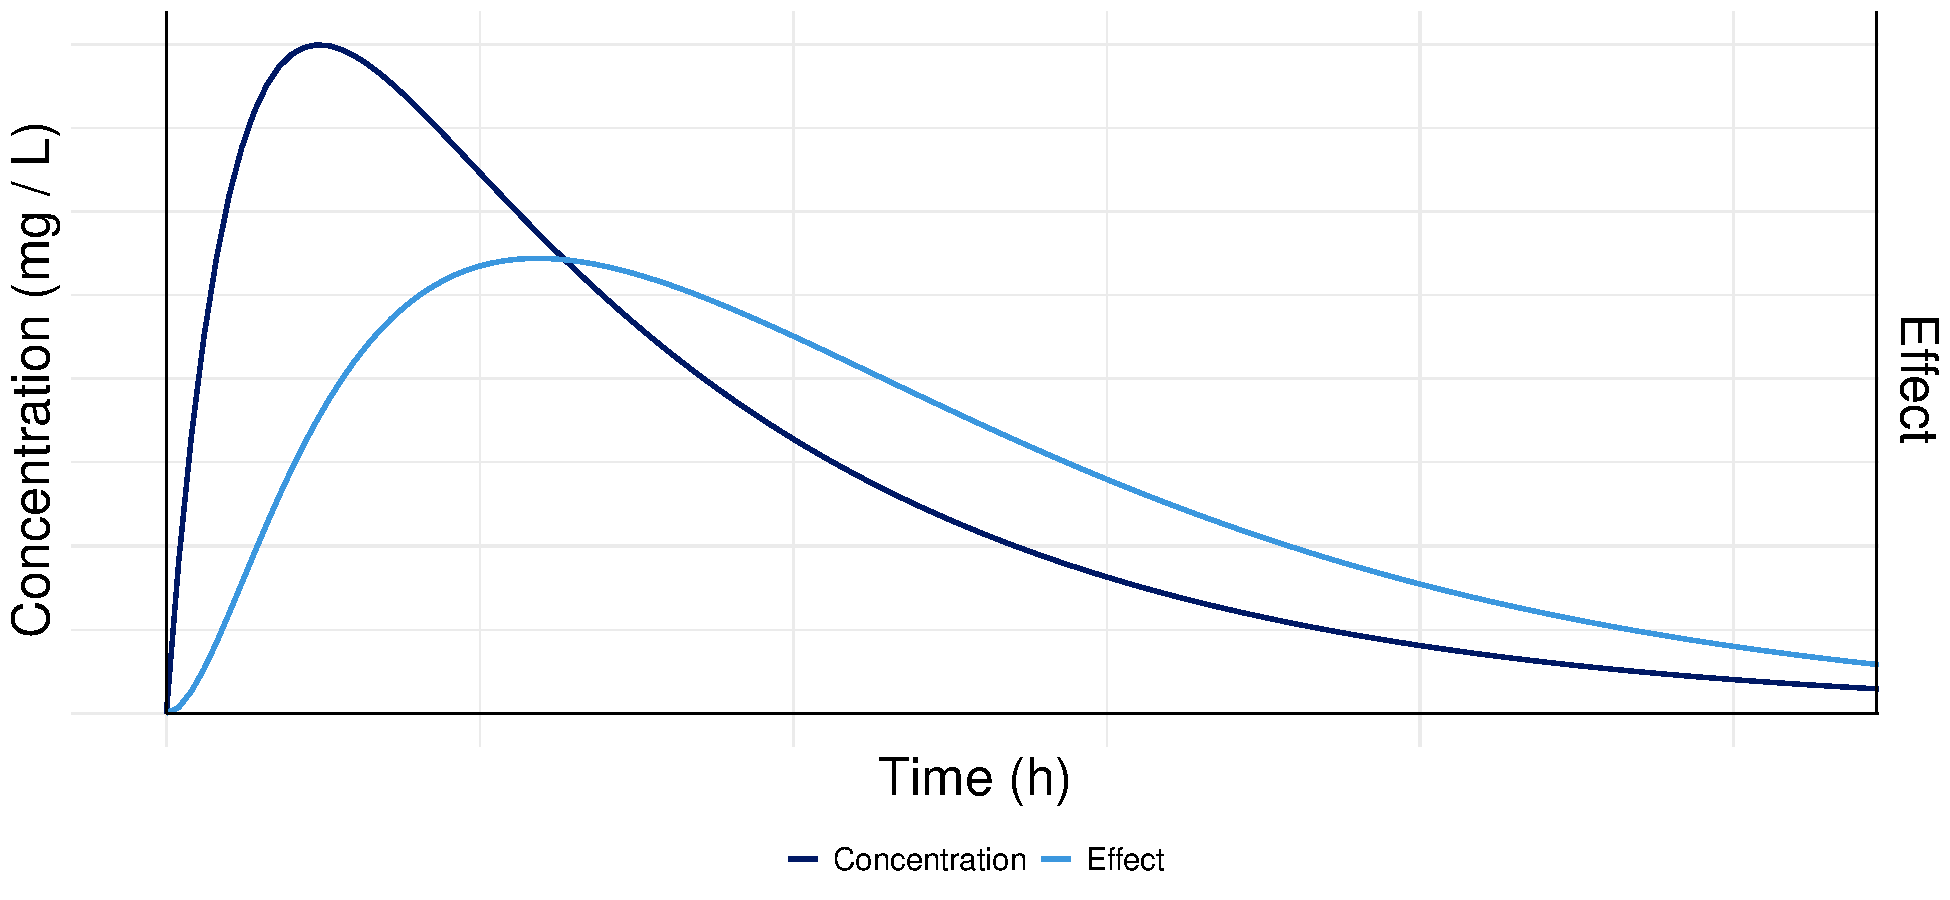
\includegraphics[width=0.95\linewidth]{fig/img/PD/PK-PDmodel.pdf}
    \caption{Concentration and effect relationship of a one-compartment PK model administered EV, incorporating an effect compartment.}
    \label{fig: PKPDmodel}
\end{figure}
Figure \ref{fig: PKPDmodel} shows that the inclusion of an effect compartment in the estimation leads to a delayed effect relative to the concentration levels. \citep{f11a2bf72b3e4305be6ebfffc456fc23}

\section{PK/PD-modelling} \label{sec: PK/PD-modelling}

Sequential PK/PD-modelling is an approach where PK parameters are estimated first using plasma concentration data, and then fixed to fit the PD model.

Simultaneous PK/PD-modelling combines the PK and PD models, and, in addition, allows the effect to be delayed relative to the concentration level measured in the plasma. Given a compartmental PK model, the delay in effect can be modelled by including a hypothetical effect compartment, which distributes a negligible amount of concentration from and to the central compartment, see Figure \ref{fig: One-compartment model with effect}, thus having no impact on the concentration within the central compartment. \begin{figure}[H]
    \centering
    \begin{tikzpicture}[node distance=1cm, >=Stealth, thick, scale=1, transform shape] % Smaller figure
      % Absorption Model
      \node[draw, fill=white!10, minimum width=2.5cm, minimum height=1.2cm, align=center] (absorption) {Depot};
      \node[draw, fill=gray!10, minimum width=2.5cm, minimum height=1.2cm, right=1.5cm of absorption, align=center] (central) {Central};
      \node[draw, fill=gray!15, minimum width=2.5cm, minimum height=1.2cm, above=1.5cm of central, align=center] (effect) {Effect};

      % Arrows for Absorption Model
      \node[above=0.6cm of absorption] (labelFA) {$\ F \cdot D$}; % Moved label higher
    \draw[<-] (absorption.north) ++(0,-0.36) -- ++(0,1);
    \draw[->] (absorption.east) -- (central.west) node[midway, above] {$k_a$};
    \draw[->] (central.south) -- ++(0,-1) node[midway, right] {$k_e$};

    \draw[dotted, ->] (central.north) ++(0.1,0) -- ++(0,1.5) node[midway, right] {$k_{e1}$};
    
    % Second Arrow (bottom) with vertical shift
    \draw[dotted, <-] (central.north) ++(-0.1, 0) -- ++(0,1.5) node[midway, left] {$k_{e0}$};


    \end{tikzpicture}
    \caption{One compartment model with absorption site and effect compartment.}
    \label{fig: One-compartment model with effect}
\end{figure}
The PD model can then be fitted as a sigmoid $E_{\text{max}}$ model with $C=C_e$, the solution to the ODE
\begin{align} \label{eq: Concentration in effect compartment}
    \Dif{C_e}(t) = k_{e1} * C_{\text{c}}(t) - k_{e0} C_e(t),
\end{align}
where $C_e$ and $C_c$ denote the concentration of drug in the effect and central compartment, respectively, and $k_{e1}$ and $k_{e0}$ denote the distribution of drug to and from the effect compartment from and to the central compartment, respectively. 

The simultaneous PK/PD modelling allows for $C_c$ and $C_p$ to be modelled together in a system of ODEs, ensuring that the PK profile dynamically influences the PD response.

Drug concentration within the central compartment and effect estimated using the Sigmoid Emax model on the concentration in the effect compartment, is depicted in Figure \ref{fig: PKPDmodel}.
\begin{figure}[H]
    \centering
    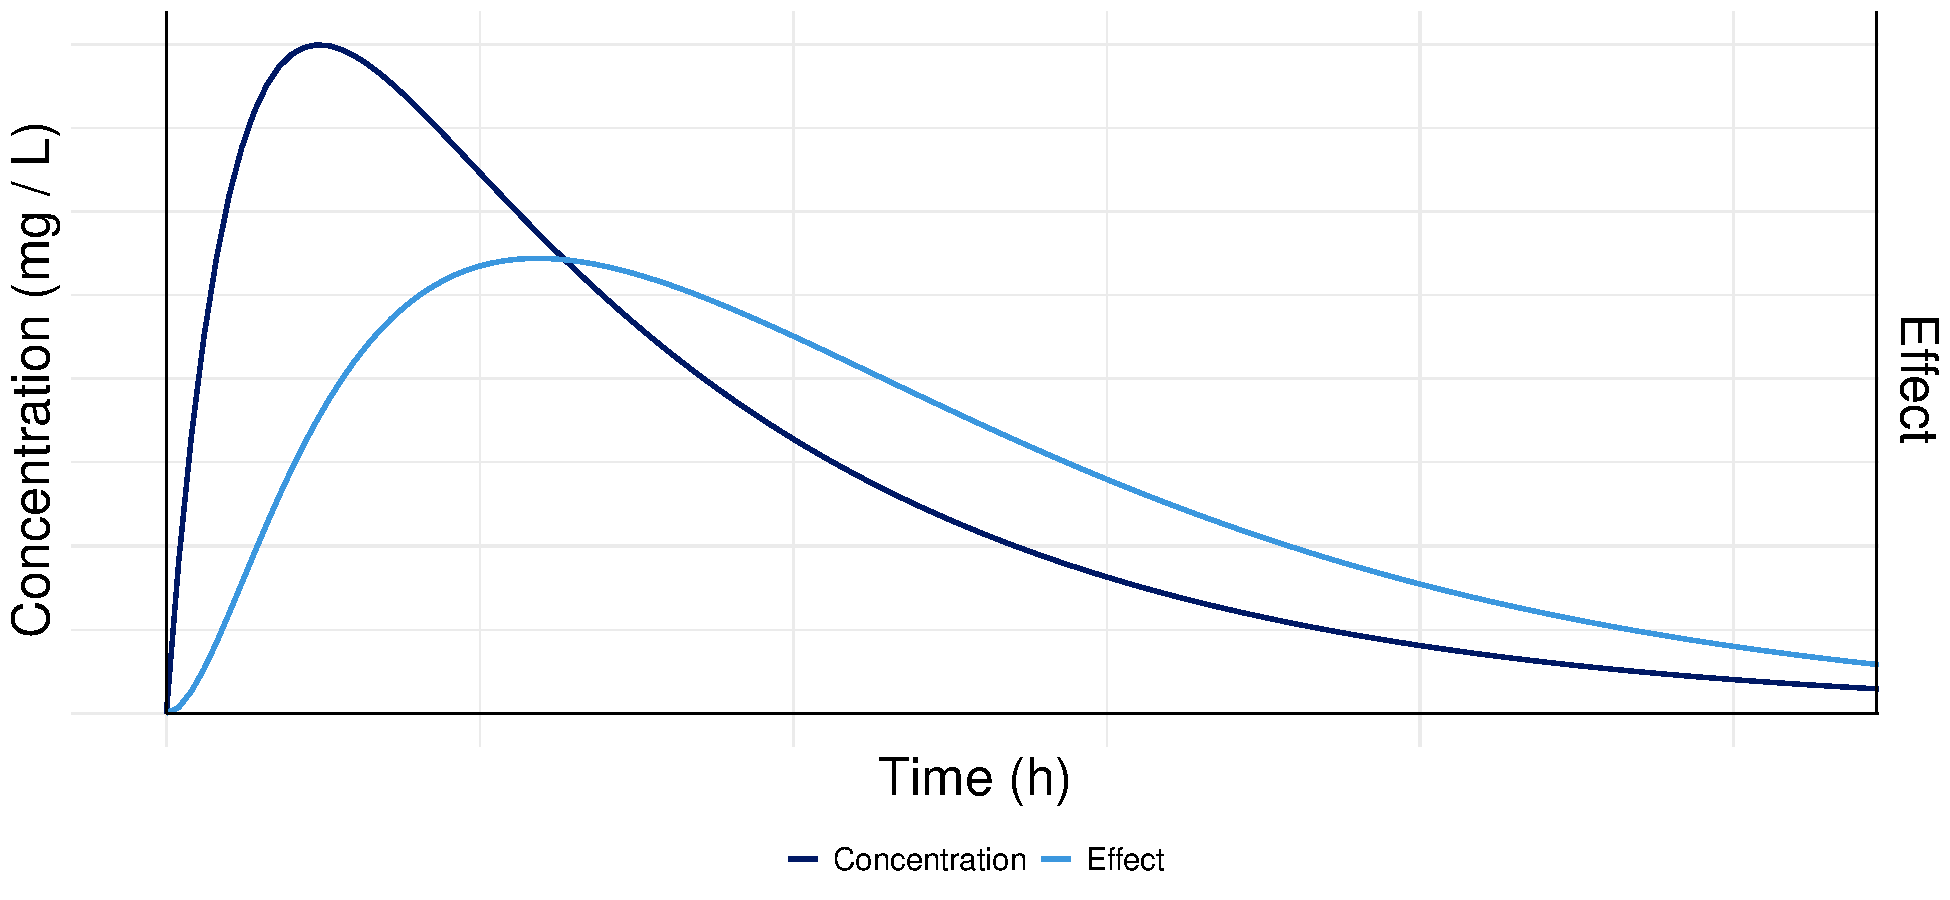
\includegraphics[width=0.95\linewidth]{fig/img/PD/PK-PDmodel.pdf}
    \caption{Concentration and effect relationship of a one-compartment PK model administered EV, incorporating an effect compartment.}
    \label{fig: PKPDmodel}
\end{figure}
Figure \ref{fig: PKPDmodel} shows that the inclusion of an effect compartment in the estimation leads to a delayed effect relative to the concentration levels. \citep{f11a2bf72b3e4305be6ebfffc456fc23}
\chapter{Non-Linear Mixed Models}
Non-linear mixed models (NLMMs) in pharmacometrics (PMX) estimate PK and PD parameters by modelling compartment dynamics.


\section{The Non-Linear Mixed Model} \label{sec: The Non-Linear Mixed Model}
Consider $N \in \N$ subjects observed over a time interval, $T=[t_{start},t_{end}] \subseteq \R^+$, where each subject $i \in \{1,2,\dots,N\}$ is measured $n_i \in \N$ times at time points $t_{i,1},t_{i,2},\dots,t_{i,n_i} \in T$. The response of subject $i$, measured at time point $t_{i,j} \in T$, is represented by $y_{i,j} \in \R$, such that $y_i=(y_{i,1},\dots,y_{i,n_i})^\top$ contains all $n_i$ responses from subject $i$. Additionally, let $x_i=(u_i^\top,a_i^\top)^\top$ denote the covariates associated with subject $i$, where $a_i$ encompasses subject-specific covariates (e.g. weight, age, sex), and $u_i$ comprises non-subject-specific covariates (e.g. dose). The resulting dataset comprises observations $\left\{(y_i,x_i) \mid  \ i =1,2,\dots,N\right\}$, assumed to be independent across $i$.

An NLMM can, for $j \in \{1,2,\dots,n_i\}$, $i \in \{1,2,\dots,N\}$, be written as the two-stage model
\begin{align}
    y_i &= g(t,u_i,\theta_i)+e_i, \quad e_i\mid \theta_i \sim (0,R_i(u_i,\theta_i,\xi)), \label{eq: NLME Stage 1}\\
    \theta_i &= d(a_i,\beta,\eta_i), \quad \eta_i \sim (0,\Omega)\label{eq: NLME Stage 2},
\end{align}
where $g$ is a non-linear function with $g(t,u_i,\theta_i):=[g(t_{i,1}, u_i, \theta_i),  \dots, g(t_{i,n_i}, u_i, \theta_i)]^\top \in \R^{n_i}$, $\theta_i \in \R^p$ is a vector of subject-specific parameters, $\xi=(\sigma,\psi^\top)^\top$ is a vector of residual variance parameters, $d$ is a function with $d(a_i,\beta,\eta_i) \in \R^p$, $\beta \in \R^k$ is a vector of fixed-effect parameters, $\eta_i \in \R^r$ is a vector of random effects associated with subject $i$, and $e_i = (e_{i,1}, e_{i,2}, \dots, e_{i,n_i})^\top \in \R^{n_i}$ is a vector of random errors for measurements within subject $i$ \citep[pp. 392-393]{Davidian2003}. The parameters to be estimated are $\Theta = \{\beta, \xi, \Omega\}$.

Stage 1, represented by \eqref{eq: NLME Stage 1}, characterises the within-subject variation by modelling the inherent tendency for the response of subject $i$, $\Ex{y_{i} \mid \theta_i} = g(t,u_i,\theta_i)$, over time \citep[pp. 395-396]{Davidian2003}. An example of a stage 1 model can be seen in Example \ref{ex: Stage 1 NLME}. Conversely, stage 2, represented by \eqref{eq: NLME Stage 2}, models the between-subject variability (BSV) in $\theta_i$, due to systematic association with covariates in $a_i$, and random variation within the population, represented by $\eta_i$ \citep[p. 393]{Davidian2003}. An example of a stage 2 model can be seen in Example \ref{ex: Stage 2 NLME}. 

\begin{exmp}{Stage 1: Within-Subject Variation}
Consider a one-compartment model with EV administration of a single dose. The amount of drug at time $t$ is given by \eqref{eq: sol to first order kinetic of amount in one com without abs}. Assuming $F=1$, the concentration for subject $i$ at time $t_{i,j}$ is given by 
\begin{align}
        C_{c,i}(t_{i,j}) &= \frac{k_{a,i} D_i}{V_{i}(k_{a,i} - CL_i/V_{i})} \left( \exp(-CL_i/V_{i} * t_{i,j}) - \exp(-k_{a,i} * t_{i,j}) \right).\label{eq: conc. one-comp with abs, F=1}
\end{align}
The function \eqref{eq: conc. one-comp with abs, F=1} is an example of  $g(t_{i,j}, u_i, \theta_i)$ specified in \eqref{eq: NLME Stage 1} with $u_i=D_i$ and $\theta_i=(k_{a,i}, V_{i}, Cl_i)^\top$ \citep[pp. 388-389]{Davidian2003}. 
\label{ex: Stage 1 NLME}
\end{exmp}

\section{The Covariate Submodel} \label{sec: covariate model}

% Introduction

% Conversely, stage 2, represented by \eqref{eq: NLME Stage 2}, addresses the between-subject variation by characterising how $\theta_i$ varies among subjects, due to systematic association with covariates in $a_i$, and random variation within the population, represented by $\eta_i$. An example of a stage 2 model can be seen in Example \ref{ex: Stage 2 NLME}.

% The population model can be composed into two parts; the covariate model and the random effects $\eta_i$. Firstly, the covariate model will be elaborated.
% The aim is to include covariates that help explain the between subject variability (BSV) and thereby decrease the residual variance. It  will not be elaborated how to asses whether it is appropriate to include a covariate or not.

% The function $h$ in \eqref{eq: NLME Stage 2} allow the subject-specific parameters, $\theta_{i}$ to be modelled with $a_i$ as predictors. In order to include each covariate appropriately $h$ may be composed of $p$ unique functions for each of the parameters in $\theta_i$. How the covariates are incorporated depends on the type of covariate i.e. if it is continuous or categorial.
The function $d$ in \eqref{eq: NLME Stage 2} is composed of $p$ functions to appropriately model each of the subject-specific parameters in $\theta_{i}$ using fixed and random effects. 
% Intro random effects
% Modelling the random effect, $\eta_i$, introduced in \eqref{eq: NLME Stage 2} will now be further elaborated. If a parameter is modelled as fixed effect then the subject-specific parameter will be the same for all subjects. This assumption may not be appropriate for all parameters and will depend on the type of parameter and data collected. The covariate model allow the subject-specific parameters to vary based on the subjects covariates. However there might be between subject variability (BSV), also known as inter-subject variability, that can be captured by including random effects to quantify the variability in the population. 
% However, if too little data is collected it might not be possible to capture the variation or model the random effects. 

% If otherwise not. E.g. if a covariate is included in multiple subject-specific parameters modelled as random effects $\Omega$ might not be diagonal.
%as a fixed effect

It is appropriate to model parameters in $\theta_{i}$ as fixed effects if the data collected is sparse, or if it is a reasonable assumption to make about the parameter \citep[p. 238]{bonate}.

% BSV
It is common to model PK parameters with random effects on the exponential scale to ensure positivity of $\theta_{i}$ \citep[p. 238]{bonate} , e.g., for $p = k = r = 1$, 
%$\theta_{i}, \eta_{i}, \beta_{\mu} \in \R$,
\begin{align*}
    \theta_{i} &= \beta_{\mu} \exp(\eta_{i}),
    %\theta_{i,2} &= \beta_{2, \mu} \exp(\eta_{2i}),
\end{align*}
where $\beta_{\mu}$ is the population mean of $\theta_{i}$, which can be substituted with a model using covariates.
Random effects modelled on the arithmetic scale are more common for PD parameters \citep[p. 240]{bonate}, e.g., for $p = k = r = 1$, 
\begin{align*}
     \theta_{i} &= \beta_{\mu} + \eta_{i}.
\end{align*}
When parameters are modelled on different scales, the 
elements in $\Omega$ are not directly comparable.

If the elements in $\theta_i$ modelled as random effects are independent, $\Omega$ is diagonal. 
If a pair of parameters in $\theta_i$ are highly correlated, it can be accounted for by a shared random effect \citep[p. 239]{bonate}, e.g., for $p = 2$, $k = 3$, and $r = 1$,
%$\eta_{i} \in \R$ $\beta \in \R^2$ and $\theta_i \in \R^3$
\begin{align*}
    \theta_{i,1} &= \beta_{1, \mu} \exp(\eta_{i,1}), \\
     \theta_{i,2} &= \beta_{2, \mu} \exp(\beta_3 \eta_{i,1}),
\end{align*}
where $\beta_3 = \frac{\omega_{22}}{\omega_{11}}$, i.e the ratio of standard deviations, resulting in $\Omega$ being a scalar. If the correlation is smaller, an approach is to include a common random effect \citep[p. 240]{bonate}, e.g., for $ p = k = r = 2$,
\begin{align*}
    \theta_{i,1}  & = \beta_{1\mu} \exp(\eta_{i,1}), \\
     \theta_{i,2} & = \beta_{2\mu} \exp(\eta_{i,2} + \eta_{i,1}).
\end{align*}
which results in $\Omega$ having non-zero off-diagonals.

\begin{exmp}{Stage 2: Between-Subject Variation}
Consider the one-compartment model from Example \ref{ex: Stage 1 NLME}. If each subject has covariates $a_i=(w_i,\text{sex}_i)^\top$, where $w_i$ is the weight (kg) of subject $i$, and $\text{sex}_i=1$ if subject $i$ is male, and  $0$ otherwise, then an example of \eqref{eq: NLME Stage 2}, with $\eta_i=(\eta_{i,1},\eta_{i,2},\eta_{i,3})^\top$ is \label{ex: Stage 2 NLME}
\begin{align*}
    k_{a,i}&=\exp(\beta_1+\eta_{i,1}),\\
    V_{i}&=\exp(\beta_2+\beta_3w_i+\eta_{i,2}),\\
    Cl_i &= \exp(\beta_4+\beta_5w_i+\beta_6\text{sex}_i+\beta_7w_i\text{sex}_i+\eta_{i,3}).
\end{align*}
\end{exmp}
% IOV
In addition to BSV, inclusion of random effects also enables capturing inter-occasion variability (IOV), which is relevant when a certain occasion affects the variability in a parameter in $\theta_i$ \citep[pp. 241-243]{bonate}, e.g., for $p = 1$, $k = 1$, $r = s + 1$, and $s \in \N$,
% \begin{align} \label{eq: IOV with studies}
%     \theta_i = \theta_\mu\exp(\eta_i + \eta_1 \text{OCC}_1 + \cdots + \eta_s \text{OCC}_s).
% \end{align}
\begin{align} \label{eq: IOV with studies}
    \theta_{i} = \beta_\mu \exp(\eta_{i,1} + \eta_{i,2} \text{OCC}_1 + \cdots + \eta_{i,s+1} \text{OCC}_s),
\end{align}
where OCC$_1$, \dots , OCC$_s$ are binary variables taking either the value one if the subject is associated with the given occasion and zero otherwise.

There are multiple methods to include random effects, and their incorporation should align with the given context.

% standardisation and collinearity
To ensure stability of the optimisation process and interpretability of the parameters, it is common to normalise, scale, or center continuous covariates \citep[p. 249]{bonate}. Furthermore, collinearity should be avoided, as \cite{Bonate1999} concluded that including a pair of collinear covariates results in unstable and biased parameter estimates.

% Continuous covariates
A continuous covariate, $a_{i1} \in \R$, can be included in an additive, exponential, or power model, e.g., for $p = 1$, $k = 2$, and $r = 0$,
\begin{align} 
    \theta_{i} = \begin{cases}
        \beta_{1} + \beta_{2} a_{i,1}  & \text{additive}, \\ 
    \beta_{1} \exp( \beta_{2}  a_{i,1}) \quad & \text{exponential}, \\ 
    \beta_{1} ( a_{i,1} )^{\beta_{2}} & \text{power}.\label{eq: continuous covariate model} 
    \end{cases}
\end{align}
% \begin{align} 
%     \theta_{i} & = \beta_{1} + \beta_{2} a_{i1},\label{eq: additive continuous covariate model}  \\ 
%     \theta_{i} & = \beta_{1} \exp( \beta_{2}  a_{i1}),\label{eq: exp continuous covariate model} \\ 
%     \theta_{i} & = \beta_{1} ( a_{i1} )^{\beta_{2}} \label{eq: power continuous covariate model}
% \end{align}
The additive model is used if a linear relation is present, while the exponential or power model is used if the relation is curvilinear. If $\theta_{i}$ is restricted to be positive, the exponential model is the appropriate model specification.

% Categorical covariates
The additive model from \eqref{eq: continuous covariate model} can be extended to include a categorical covariate, $a_{i,2} \in \{ 0, 1 \}$, modelled additively, exponentially, or fractionally, e.g.,
\begin{align}
    \theta_{i}  = 
    \begin{cases}
        \beta_{1} + \beta_{2} a_{i,1} + \beta_3 a_{i,2} & \text{additive}, \\
        (\beta_{1} + \beta_{2} a_{i,1} ) \exp(\beta_3 a_{i,2}) \quad & \text{exponential}, \\
      (\beta_{1} + \beta_{2} a_{i,1} ) ( 1 + \beta_3 a_{i,2}) & \text{fractional}. \\
    \end{cases}
    \label{eq: frac categorical covariate model}
\end{align}
% This is a simple example how to incorporate a continuous covariate and a binary categorical covariate. 
The setting naturally expands to include more than two covariates. When multiple covariates are included, it should be considered whether the covariates share an additive, multiplicative or interactive relation.
Multiplicative relations are often modelled on log-scale in which the relation is additive. 

The choice of $d$ is typically determined by visual inspection of covariates vs. $\hat{\theta}_{i}$, modelled as an intercept, fitted by \eqref{eq: NLME Stage 1}, and by comparing values from objective functions.
However, in a PK/PD setting, the covariate model must be interpretable.
When $d$ is specified, it is substituted into \eqref{eq: NLME Stage 1}.
% \begin{align}
%     \theta_{i} & = \beta_{1} + \beta_{2} a_{i1} + \beta_3 a_{i2},\label{eq: additive categorical covariate model}  \\ 
%      \theta_{i} & =  ( \beta_{1} + \beta_{2} a_{i1} ) \exp ( \beta_3 a_{i2} ), \label{eq: exp categorical covariate model}  \\
%     \theta_{i} & =  ( \beta_{1} + \beta_{2} a_{i1} ) ( 1 + \beta_3 a_{i2} ).
% \end{align}

% \begin{align}
%    \theta_i = \begin{cases}
%        \beta_{1} + \beta_{2} a_{i1} + \beta_3 a_{i2} & \text{additive}  \\ 
%      ( \beta_{1} + \beta_{2} a_{i1} ) \exp ( \beta_3 a_{i2} ) \quad & \text{exponential}  \\
%     ( \beta_{1} + \beta_{2} a_{i1} ) ( 1 + \beta_3 a_{i2} ) & \text{fractional change}.
%     \end{cases}
% \end{align}

% \begin{align}
%     \theta_{i1} & = \beta_{1} + \beta_{2} a_{i1} + \beta_{3} a_{i2},\label{eq: linear covariate model}  \\ 
%     \theta_{i2} & = \beta_{4} \exp( \beta_{5} a_{i1} + \beta_{6} a_{i2}),\label{eq: exp covariate model} \\ 
%     \theta_{i3} & = \beta_{7} ( a_{i1} )^{\beta_{8}} (1 + \beta_{
%     9} a_{i2}). \label{eq: power covariate model}
% \end{align}


%The parameters associated with the covariates will change under scaling and the intercept will change under centering.
%This transformation of the predictors can improve stability in the optimisationprocess \citep[p. 249]{bonate}. Transforming the predictors might also improve interpretation of the covariate model by having a reference level for the subject-specific parameter.



% \section{Residual variability}
% The unexplained variability of a NLMM is contained in $\Var{e_i} = R_i$, for $i=1,\dots,N$, and is considered the collection of within-subject variability, measurement error, and model misspecification. The residual error can therefore be considered as the sum
% \begin{align*}
%     e_{i,j}=e^M_{i,j}+ e^S_{i,j}+e^R_{i,j},
% \end{align*}
% where $e^M_{i,j}$ denotes measurement error, $e^S_{i,j}$ denotes model misspecification, and $e^R_{i,j}$ denotes the remaining residual which captures the within-individual variation.
% \begin{figure}[H]
%         \centering
%         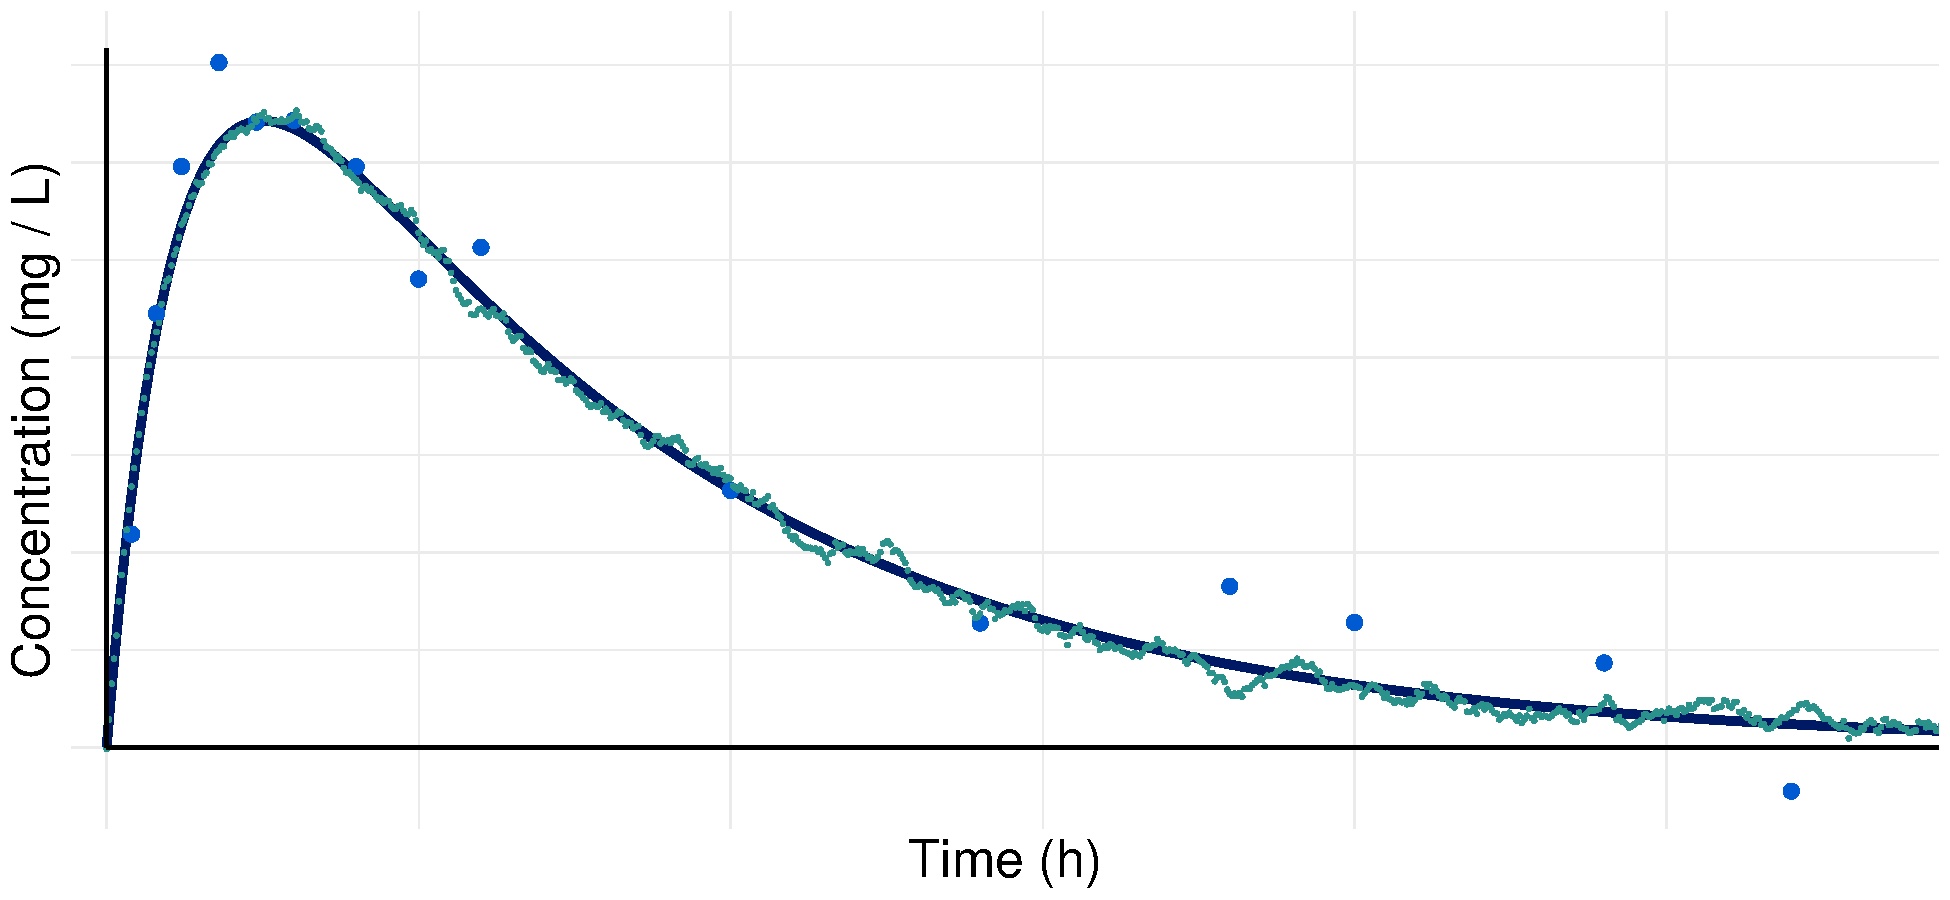
\includegraphics[width=\linewidth]{fig/img/Residual Variance Model/Measurement error.pdf}
%         \label{fig: Measurement error}
%         \caption{Concentration function, realised response profile and measurements}
%     \label{fig: Measurement error}
% \end{figure}
% If $g$ is a misspecified model, and $g +e^S_{i,j}$ is the true trajectory of the response profile, then $g$ itself is a biased representation of the true trajectory with $e^S_{i,j}$ representing systematic deviations. However, since the exact nature of the misspecification is unknown, it is hard to distinguish between bias and within-individual variation, and therefore $ e^S_{i,j}+e^R_{i,j}$ is often considered a unified source of variation. Henceforth, it is assumed that $e^S_{i,j}=0$.

% % Initially, assume that $g$ is a correctly specified model, such that $e^S_{i,j}=0$. To understand the nature of the partitioning of the residual, consider Figure \ref{fig: Measurement error}, in which the dark blue function represents $g$, whereas the blue dots represent the $n_i$ realised measurements $y_{i,j}$, and the green trajectory represents the true, but unknown, response profile of subject $i$. 

% The difference between the true response profile and $g$ is $e^R_{i,j}$; a variability mainly due to model assumptions. For instance, in a compartment model, it is assumed that the drug is being evenly distributed within the plasma, while in reality, the drug might not be perfectly mixed within the body, making the true response profile fluctuate locally around $g$ as visualised in Figure \ref{fig: Measurement error}. 

% The difference between the true response profile and the observed response measurements $y_{i,j}$ is $e^M_{i,j}$.

% Note that $g$ should be understood as an average of all possible true response profiles and measurement errors that could be observed for subject $i$, also called the inherent tendency for the response of subject $i$ over time \citep[p. 396]{Davidian2003}. This implies that NLME models are fundamentally concerned with modelling inherent tendencies of individuals, rather than the true response profiles.

% % Clearly, if it is assumed that $g$ is exactly equal to the true trajectory of the response profile, then $e_{i,j}^S+e_{i,j}^R=0$, and thus $e_{i,j}=e_{i,j}^M$.

% If the aim is to model the residuals $e^R_{i,j}$, it might make sense to allow for autocorrelation, as $e^R_{i,j}$ and $e^R_{i,j+h}$ for small $h$ would tend to be similar, while it is not the case for larger values of $h \in \Z$, as suggested by Figure \ref{fig: Measurement error}. However, within the field of PMX, the common approach is that the primary source of variation is due to $e^M_{i,j}$, and, for this reason, the term $e^R_{i,j}$ is neglected. This implies that the error that needs to be modelled is measurement error only, i.e. 
% \begin{align*}
%     e_{i,j}:=e_{i,j}^M.
% \end{align*}
% Often, it is assumed that measurement error is not autocorrelated, since it is justifiable that the error of measurement at time point $t_{i,j}$ should not depend on the error measured at time $t_{i,j+h}$ for all values of $h \in \Z$. Under this assumption,
% \begin{align}
%     \Var{e_{i} \mid \theta_i}=R_i(u_i,\theta_i,\xi) \label{eq: diag residual covariance matrix}
% \end{align}
% is a diagonal matrix depending on $u_i, \theta_i$ specified in \eqref{eq: NLME Stage 1} and \eqref{eq: NLME Stage 2}, respectively, and $\xi=(\sigma,\psi^\top)^\top$, where $\sigma$ is a constant factor, and $\psi$ is a vector of parameters. 

% Within PMX, it is assumed that measurement errors are not autocorrelated. However, it is not always plausible to assume homoscedasticity, as measurement errors often have heteroscedastic tendencies. Thus, the aim is to choose a model for the diagonal covariance matrix \eqref{eq: diag residual covariance matrix}. 

% Let $\varepsilon_i \sim (0,\sigma^2I)$ denote a random vector of dimension $n_i$. The residual error can then be represented as
% \begin{align} \label{eq: residual variance model}
%     e_{i} &=  v(t_{}, u_i, \theta_i, \psi)\varepsilon_{i},
% \end{align}
% where $v(t,u_i,\theta_i,\psi)=[v(t_{i,1},u_i,\theta_i,\psi),\dots,v(t_{i,n_i},u_i,\theta_i,\psi)]^\top \in \R^{n_i}$ denotes a function independent of $\varepsilon_i$, and $\psi$ denotes a vector of parameters. The variance of the residual error is then
% \begin{align*}
%     \Var{e_{i} \mid \theta_i} =  [v(t_{i,j}, u_i, \theta_i, \psi)]^2\sigma^2I,
% \end{align*}
% where the dependence on the random effects is emphasized through the condition on $\theta_i$. 

% The most common error models used in PMX can be seen in Table \ref{tab:error models}. 
% \begin{table}[H]
% \centering
% \begin{tabular}{>{\raggedright\arraybackslash}p{0.4\textwidth}>{\raggedright\arraybackslash}p{0.53\textwidth}}
% \toprule
% \textbf{Error model} & \textbf{Representation of $e_i$} \\
% \midrule
% Additive & $e_{i} = \varepsilon_{i}$ \\
% Proportional & $e_{i} = [g(t, u_i, \theta_i)]^2\varepsilon_{i}$ \\
% Combined additive and proportional & $e_{i} = \left( \sqrt{1-\psi + \psi g^2(t, u_i, \theta_i)}\right)\varepsilon_{i}, \quad \psi \in [0, 1]$ \\
% \bottomrule
% \end{tabular}
% \caption{Representation of the residual error, $e_i$, for the additive, proportional and combined additive and proportional error model, respectively.}
% \label{tab:error models}
% \end{table}

% The additive error model assumes constant variance, i.e. 
% \begin{align*}
%     R_i(u_i,\theta_i,\xi)=\Var{e_i \mid \theta_i}=\Var{\varepsilon_i}=\sigma^2I.
% \end{align*}
% An example of simulated data that follows the additive residual variance model can be seen in Figure \ref{fig: Residual variance model add}.

% The proportional error model allows the variance to vary over time by letting it be proportional with the non-linear function $g$,
% \begin{align*}
% R_i(u_i,\theta_i,\xi)&=\Var{e_i \mid \theta_i}=\Var{g(t,u_i,\theta_i)\varepsilon_i \mid \theta_i}=g^2(t,u_i,\theta_i,\psi)\sigma^2I\\
% &=\sigma^2 \text{diag}[g^2(t_{i,1},u_i,\theta_i), \dots, g^2(t_{i,n_i},u_i,\theta_i)].
% \end{align*}
% An example of simulated data that follows the proportional residual variance model can be seen in Figure \ref{fig: Residual variance model prop}.

% The combined additive and proportional error model exhibits properties from both models. As $\phi_k \in [0,1]$, it is possible to adjust the contribution of each model. Note that if $\psi=0$, it simplifies to an additive model, whereas if $\psi=1$, it simplifies to a proportional model. The combined additive and proportional error has covariance matrix
% \begin{align*}
% R_i(u_i,\theta_i,\xi)&=\Var{e_i \mid \theta_i}=\Var{ \left( \sqrt{1-\psi + \psi g(t, u_i, \theta_i)^2}\right)\varepsilon_{i} \mid \theta_i} \\
%     &= \left[1-\psi + \psi g(t, u_i, \theta_i)^2\right] \sigma^2I\\
%     &=\sigma^2 \text{diag}\left[(1-\psi + \psi g(t_{i,1}, u_i, \theta_i)^2),\dots,(1-\psi + \psi g(t_{i,n_i}, u_i, \theta_i)^2)\right].
% \end{align*}
% An example of simulated data that follows the combined additive and proportional residual variance model can be seen in Figure \ref{fig: Residual variance model add prop}.

% \begin{figure}[H]
%     \centering
%     \begin{minipage}{0.45\textwidth}
%         \centering
%         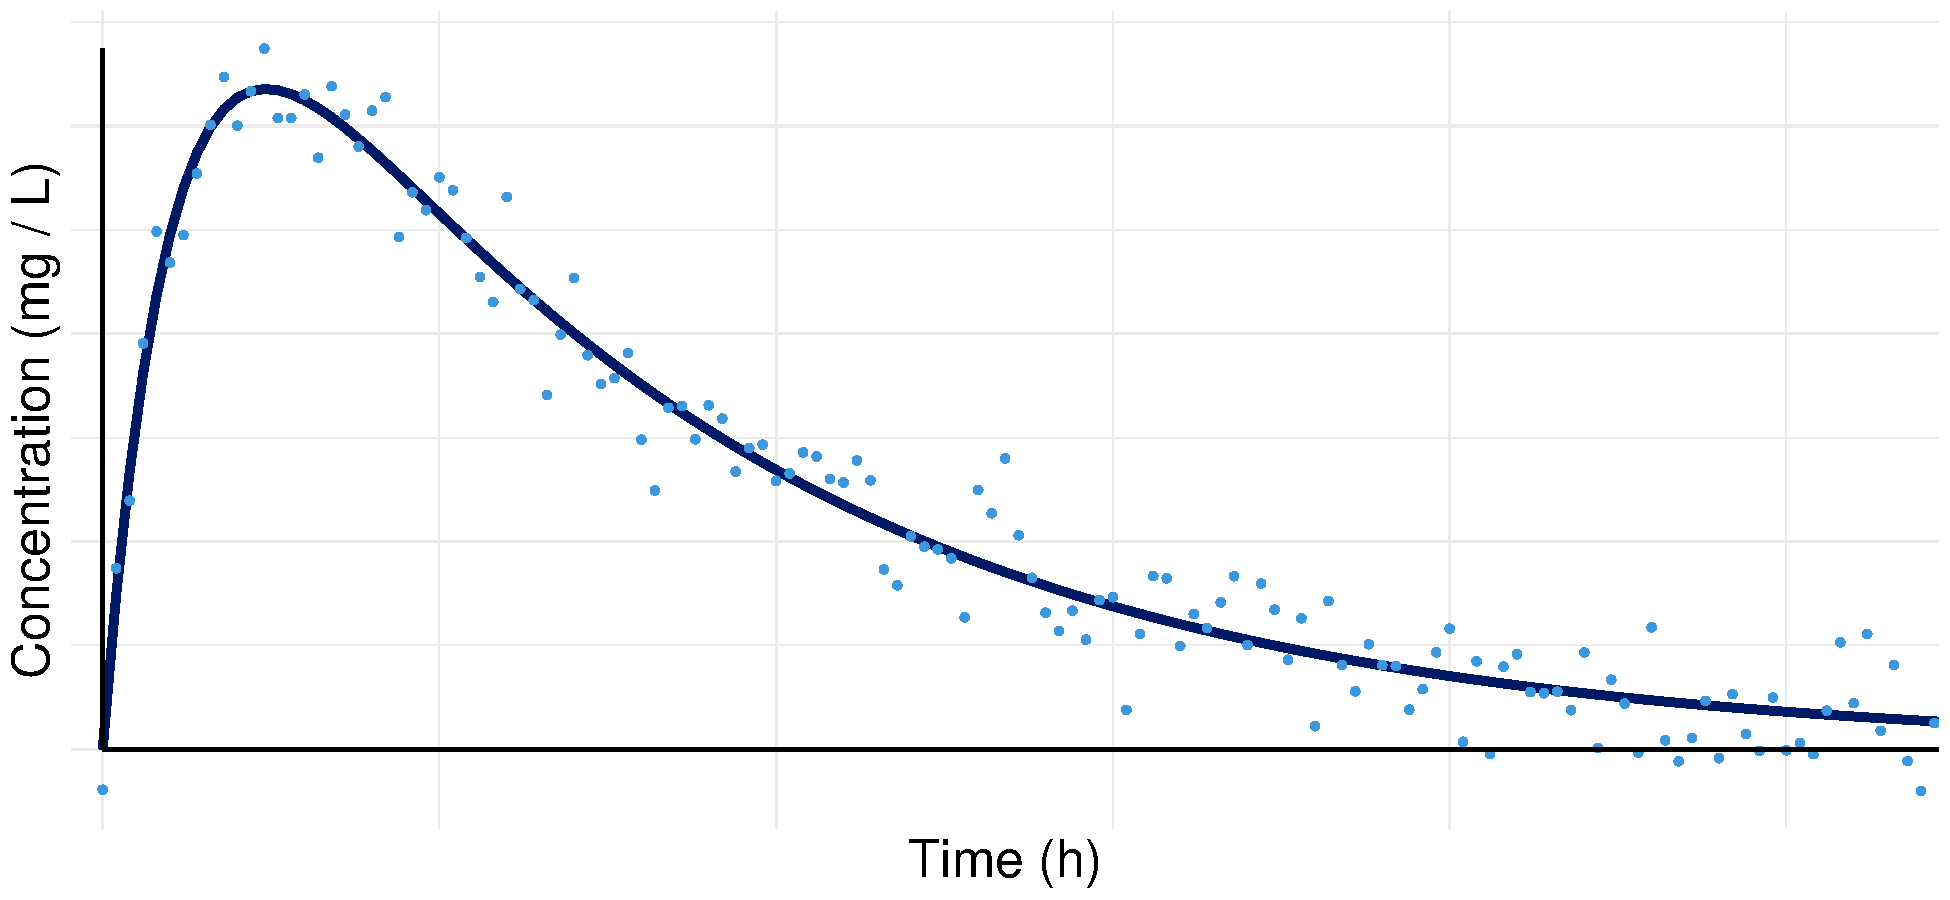
\includegraphics[width=\linewidth]{fig/img/Residual Variance Model/Concentration W. Oral Add.pdf}
%         \caption{Additive error}
%         \label{fig: Residual variance model add}
%     \end{minipage}%
%     \hfill
%     \begin{minipage}{0.45\textwidth}
%         \centering
%         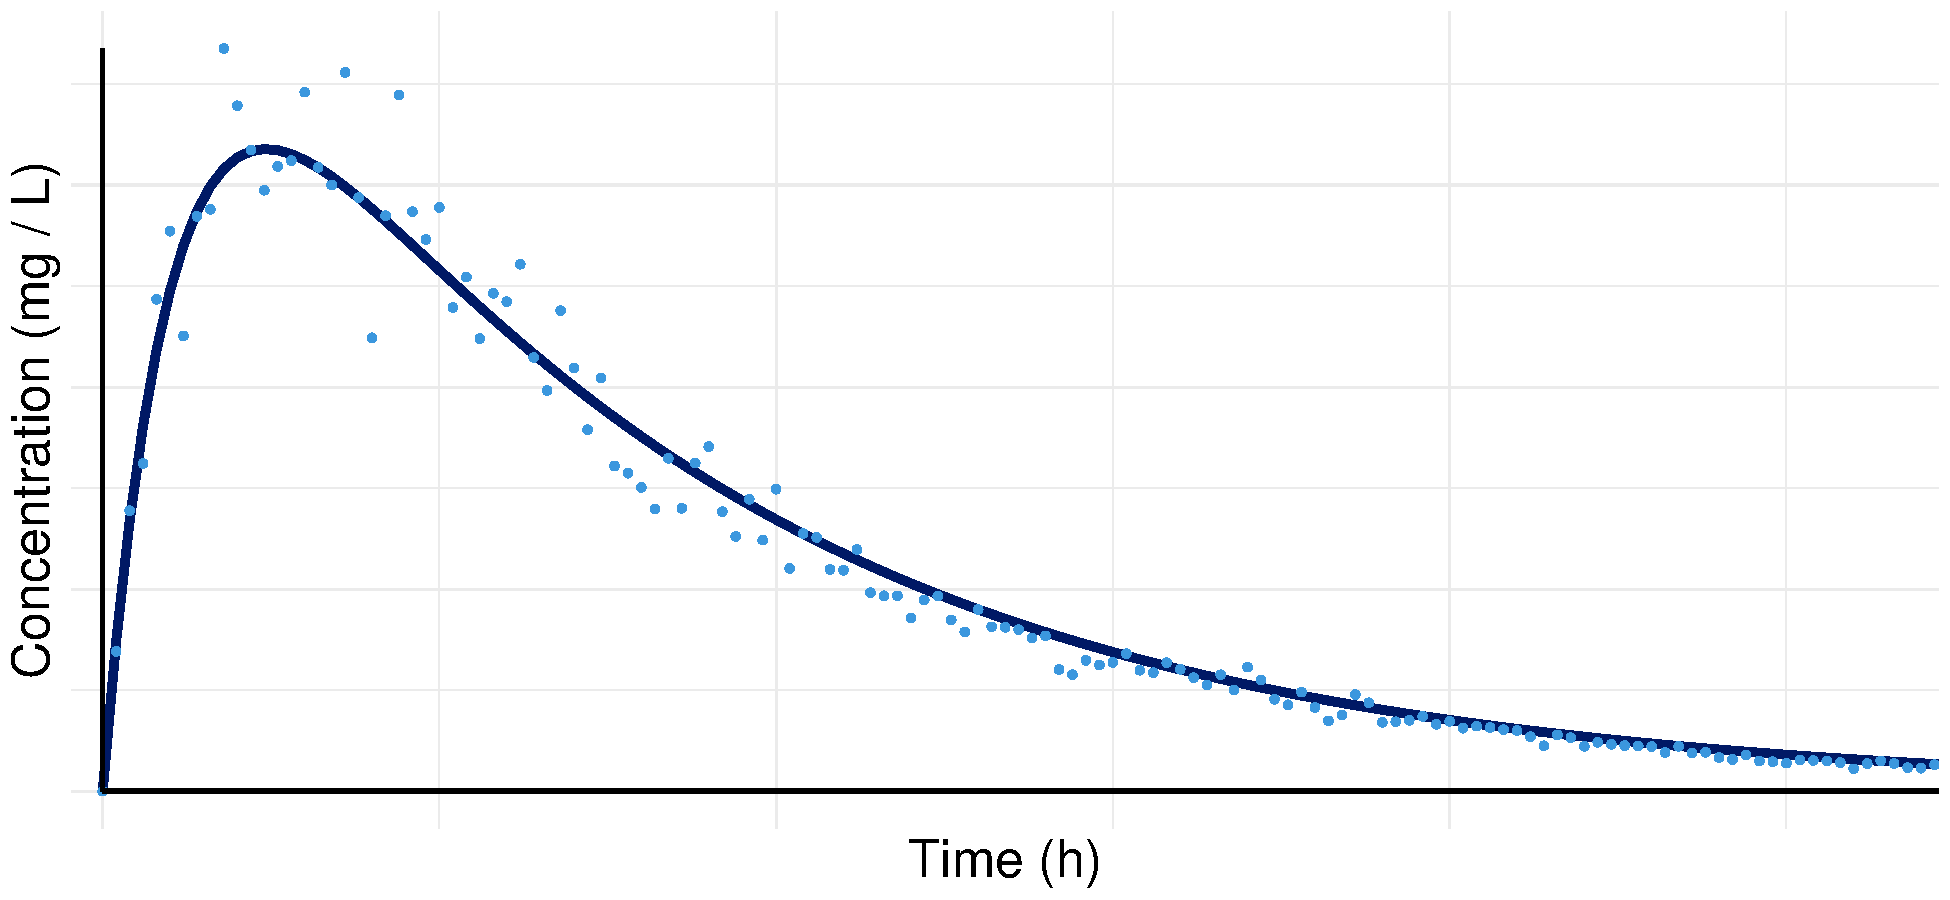
\includegraphics[width=\linewidth]{fig/img/Residual Variance Model/Concentration W. Oral Prop.pdf}
%         \caption{Proportional error}
%         \label{fig: Residual variance model prop}
%     \end{minipage}
%     \vfill

%     \begin{minipage}{0.45\textwidth}
%         \centering
%         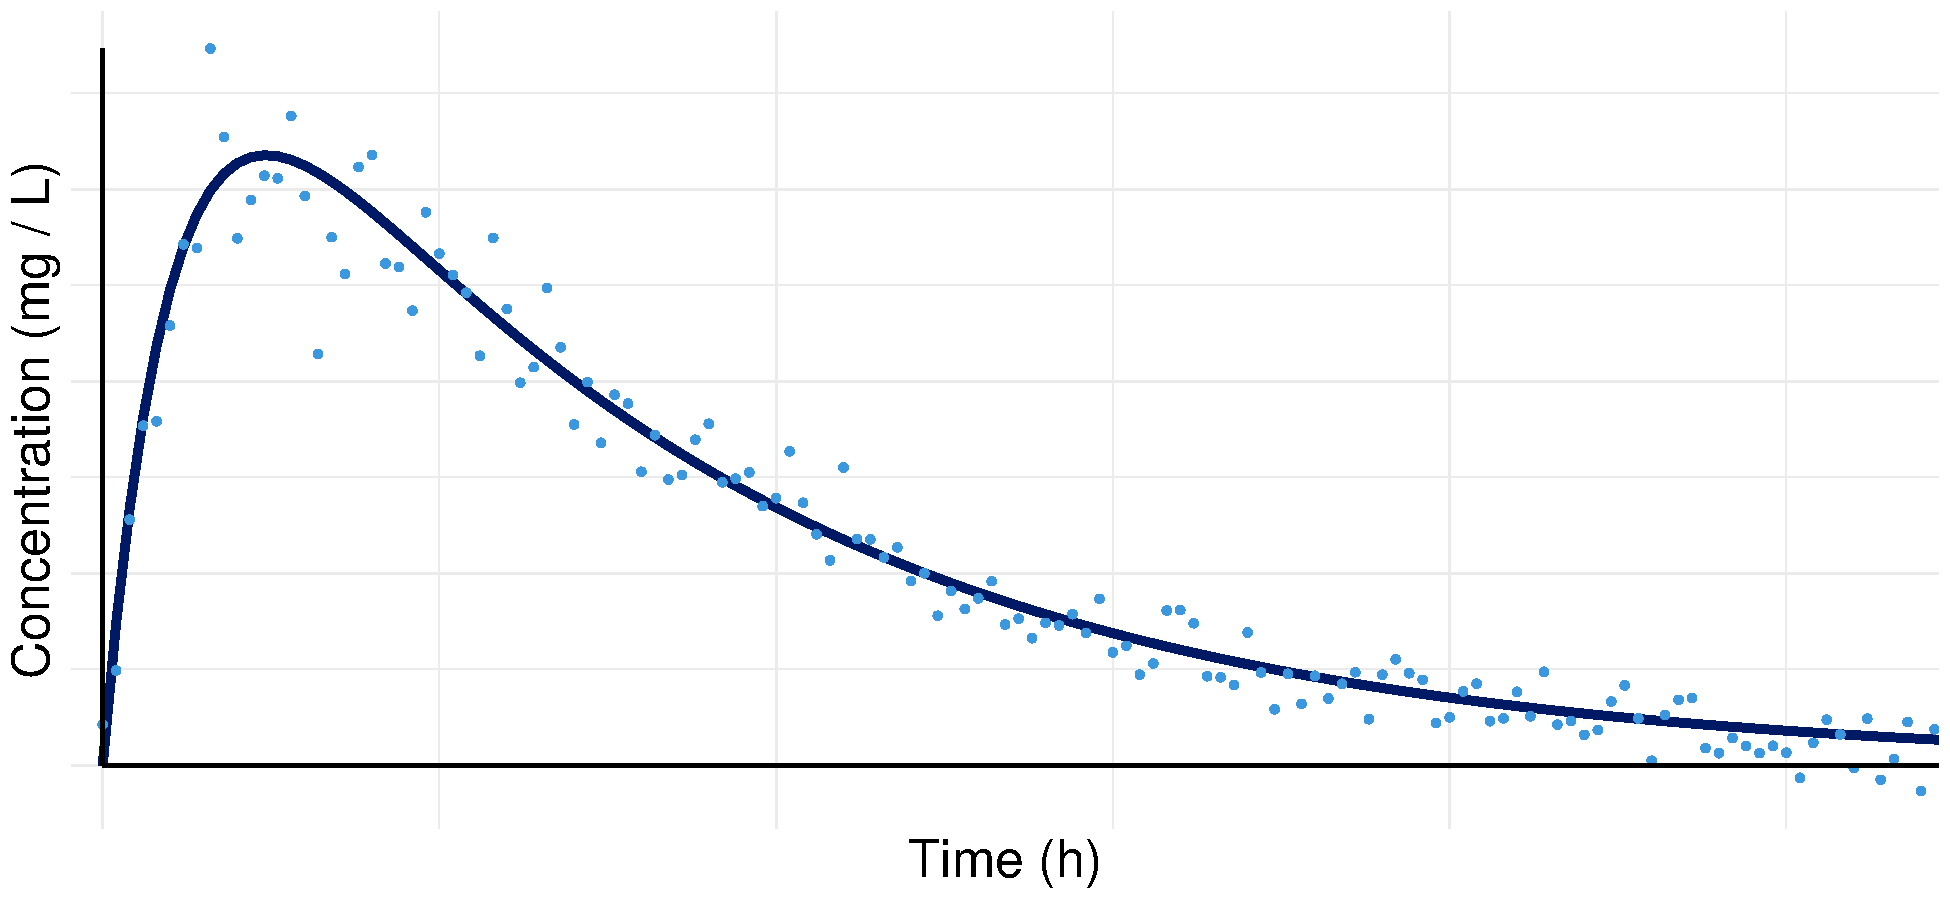
\includegraphics[width=\linewidth]{fig/img/Residual Variance Model/Concentration W. Oral Add Prop.pdf}
%         \caption{Combined additive and proportional error}
%         \label{fig: Residual variance model add prop}
%     \end{minipage}
%     \caption{Simulated concentrations from a single dose one-compartment model with EV administration, each with different error models.}
%     \label{fig: Residual variance model}
% \end{figure}
% To determine which residual variance model is most suitable, likelihood ratio tests and goodness of fit plots are used. 

\section{Residual variability}

While $\Omega \in \R^{r \times r}$ contains the BSV, the remaining unexplained variability is contained in $R_i(u_i,\theta_i,\xi)$, for $i=1,\dots,N$, and is considered the collection of within-subject variability, measurement error, and model misspecification. If $g(t_{ij},u_i,\theta_i)$ is correctly specified and $f_{ij}$ denotes the true, but unobserved, response at time $t_{ij}$, then the residual error can be considered the sum $e_{i,j}=e^M_{i,j}+e^R_{i,j}$, where $e^M_{i,j}=y_{ij}-f_{ij}$ is measurement error, and $e^R_{i,j}=f_{ij}-g(t_{ij},u_i,\theta_i)$ is within-subject variation.

In PMX, a common approximation is that residual error primarily arises from measurement error \citep{Karlsson1995}. It is standard that measurement errors at different time points, $t_{i,j}$ and $t_{i,j+h}$, are assumed independent for all $h \in \Z$, thus $R_i(u_i,\theta_i,\xi)$ is modelled as diagonal \citep[p. 398]{Davidian2003}.

In practice, measurement errors tend to vary as a function of $g(t_{ij},u_i,\theta_i)$, causing heteroscedasticity \citep[p. 398]{Davidian2003}. To account for this, it is necessary to specify an appropriate structure for $R_i(u_i,\theta_i,\xi)$. The most common error models utilised in PMX are the additive (add.), proportional (prop.), and combined add. and prop., which are detailed in Table \ref{tab:error models}. 

\begin{table}[h]
\centering
\begin{tabular}{>{\raggedright\arraybackslash}p{0.16\textwidth} >{\raggedright\arraybackslash}p{0.26\textwidth} >{\raggedright\arraybackslash}p{0.49\textwidth}}
\toprule
\textbf{Error model} & \textbf{Representation of $e_i$} & \textbf{Structure of $R_i(u_i,\theta_i,\xi)$} \\
\midrule
Add. & $\varepsilon_{i,add}$ & $\sigma^2_{add}I$ \\
Prop. & $g(t, u_i, \theta_i)\varepsilon_{i,prop}$ & $\sigma_{prop}^2 \text{diag}[g^2(t_{i,1},u_i,\theta_i), \dots, g^2(t_{i,n_i},u_i,\theta_i)]$ \\
Add./prop. & $g(t, u_i, \theta_i)\varepsilon_{i,prop}+\varepsilon_{i,add}$ & $\sigma_{prop}^2 \text{diag}[g^2(t_{i,1},u_i,\theta_i), \dots, g^2(t_{i,n_i},u_i,\theta_i)] + \sigma^2_{add}I$ \\
\bottomrule
\end{tabular}
\caption{Representation of the residual error, $e_i$, through $\varepsilon_{i,add} \sim (0,\sigma^2_{add}I)$ and $\varepsilon_{i,prop} \sim (0,\sigma^2_{prop}I)$, for the additive, proportional and combined additive and proportional error model, respectively \citep[p. 236]{bonate}.}
\label{tab:error models}
\end{table}

The additive error assumes homoscedasticity, suitable when the residual error is independent of the magnitude of $g(t_{ij},u_i,\theta_i)$. The proportional error accounts for heteroscedasticity, where the residual error increases with $g(t_{ij},u_i,\theta_i)$. When the residual error structure is uncertain, a combined additive and proportional model can be used. 

An additive error model can inappropriately yield negative concentrations, see Figure \ref{fig: Residual variance model add}, which is avoided with the proportional error model, see Figure \ref{fig: Residual variance model prop}.

% The additive error assumes constant variance, and is suitable when the residual error is independent of the magnitude of the observations. An example of simulated data that follows the additive residual variance model is depicted in Figure \ref{fig: Residual variance model add}.

% The proportional error assumes heteroscedasticity, and is suitable when the variance increases with the magnitude of the prediction. 

% If the error structure is uncertain, the combined additive and proportional error can be used instead. An example of simulated data that follows the combined additive and proportional residual variance model can be seen in Figure \ref{fig: Residual variance model add prop}.


% The structure of $R_i(u_i,\theta_i,\xi)$ for each residual variance model is shown in \ref{eq: add. error}, \ref{eq: prop error}, and \ref{eq: add prop error}, respectively. 

% The additive error model assumes constant variance, i.e. 
% \begin{align}
%     R_i(u_i,\theta_i,\xi)=\Var{e_i \mid \theta_i}=\Var{\varepsilon_{i,add}}=\sigma^2_{add}I. \label{eq: add. error}
% \end{align}
% An example of simulated data that follows the additive residual variance model can be seen in Figure \ref{fig: Residual variance model add}.

% The proportional error model allows the variance to vary over time by letting it be proportional with the non-linear function $g$,
% \begin{align}
% R_i(u_i,\theta_i,\xi)&=\Var{e_i \mid \theta_i}=\Var{g(t,u_i,\theta_i)\varepsilon_{i,prop} \mid \theta_i}=g^2(t,u_i,\theta_i,\psi)\sigma_{prop}^2I\nonumber \\
% &=\sigma_{prop}^2 \text{diag}[g^2(t_{i,1},u_i,\theta_i), \dots, g^2(t_{i,n_i},u_i,\theta_i)]. \label{eq: prop error}
% \end{align}
% An example of simulated data that follows the proportional residual variance model can be seen in Figure \ref{fig: Residual variance model prop}.

% The combined additive and proportional error model exhibits properties from both models. As $\phi_k \in [0,1]$, it is possible to adjust the contribution of each model. Note that if $\psi=0$, it simplifies to an additive model, whereas if $\psi=1$, it simplifies to a proportional model. The combined additive and proportional error has covariance matrix
% \begin{align}
% R_i(u_i,\theta_i,\xi)&=\Var{e_i \mid \theta_i}=\Var{ \left( \sqrt{1-\psi + \psi g(t, u_i, \theta_i)^2}\right)\varepsilon_{i} \mid \theta_i} \\
%     &= \left[1-\psi + \psi g(t, u_i, \theta_i)^2\right] \sigma^2I \nonumber \\
%     &=\sigma^2 \text{diag}\left[(1-\psi + \psi g(t_{i,1}, u_i, \theta_i)^2),\dots,(1-\psi + \psi g(t_{i,n_i}, u_i, \theta_i)^2)\right]. \label{eq: add prop error}
% \end{align}
% An example of simulated data that follows the combined additive and proportional residual variance model can be seen in Figure \ref{fig: Residual variance model add prop}.

\begin{figure}[h]
    \centering
    \begin{minipage}{0.45\textwidth}
        \centering
        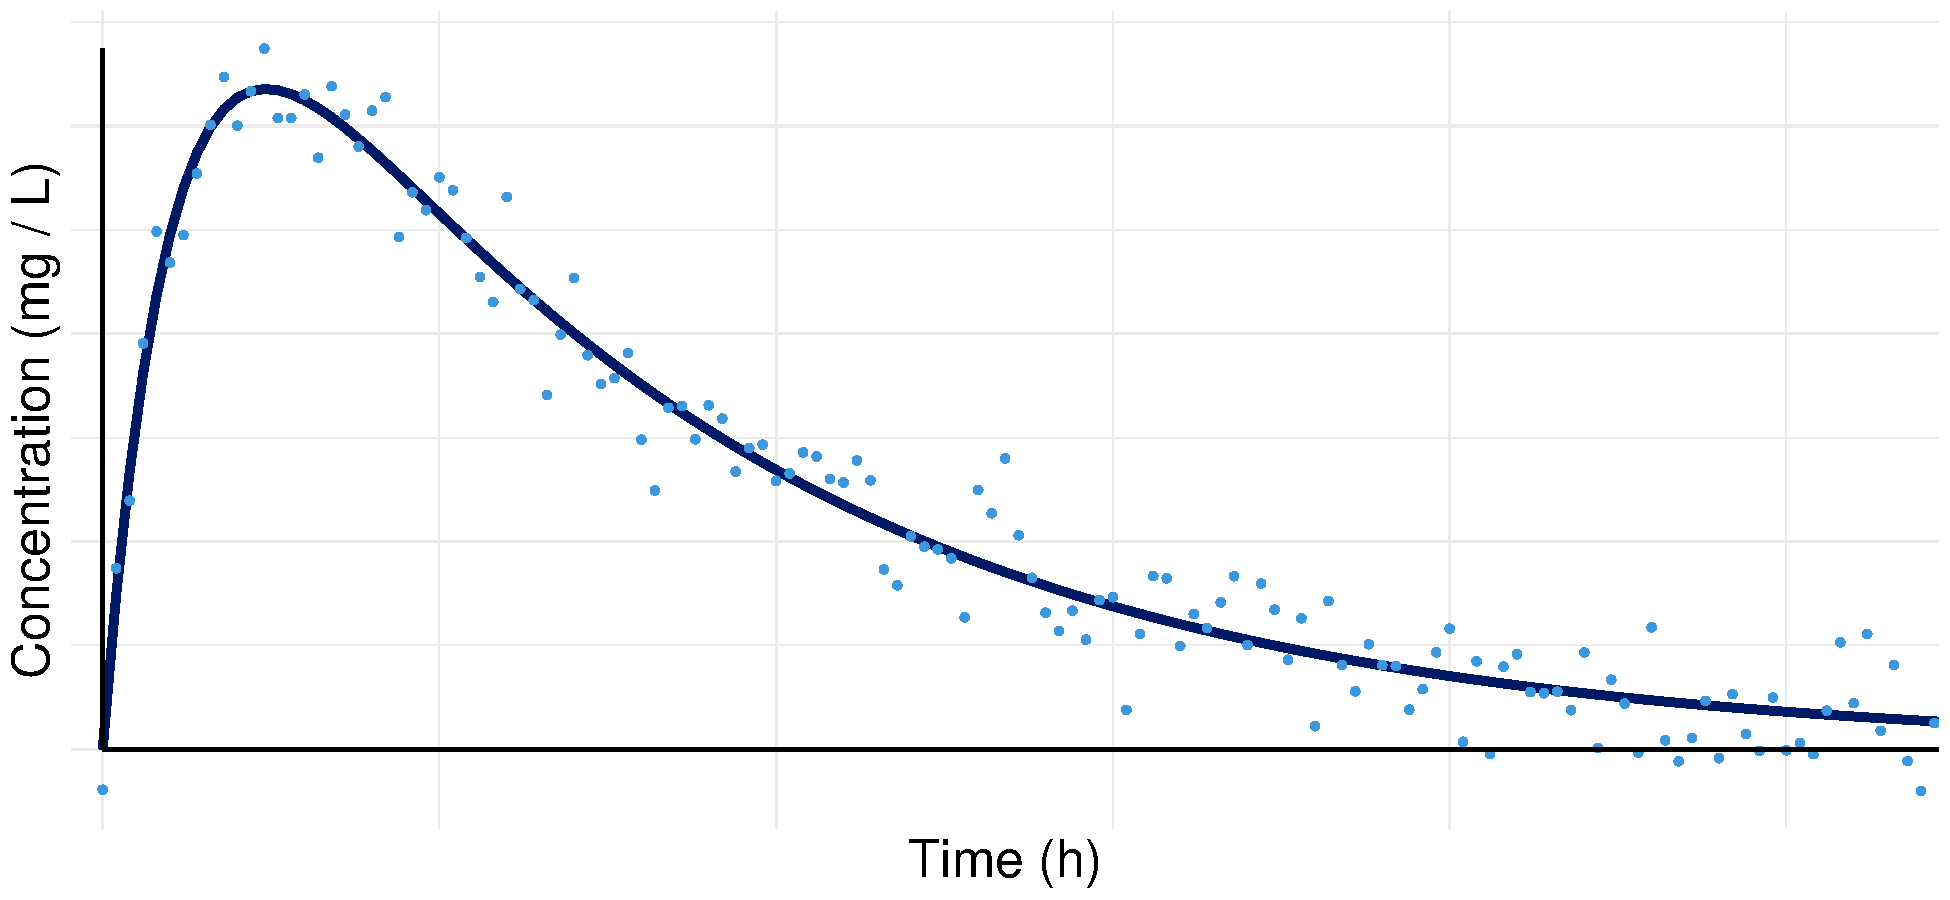
\includegraphics[width=\linewidth]{fig/img/Residual Variance Model/Concentration W. Oral Add.pdf}
        \caption{Additive error}
        \label{fig: Residual variance model add}
    \end{minipage}%
    \hfill
    \begin{minipage}{0.45\textwidth}
        \centering
        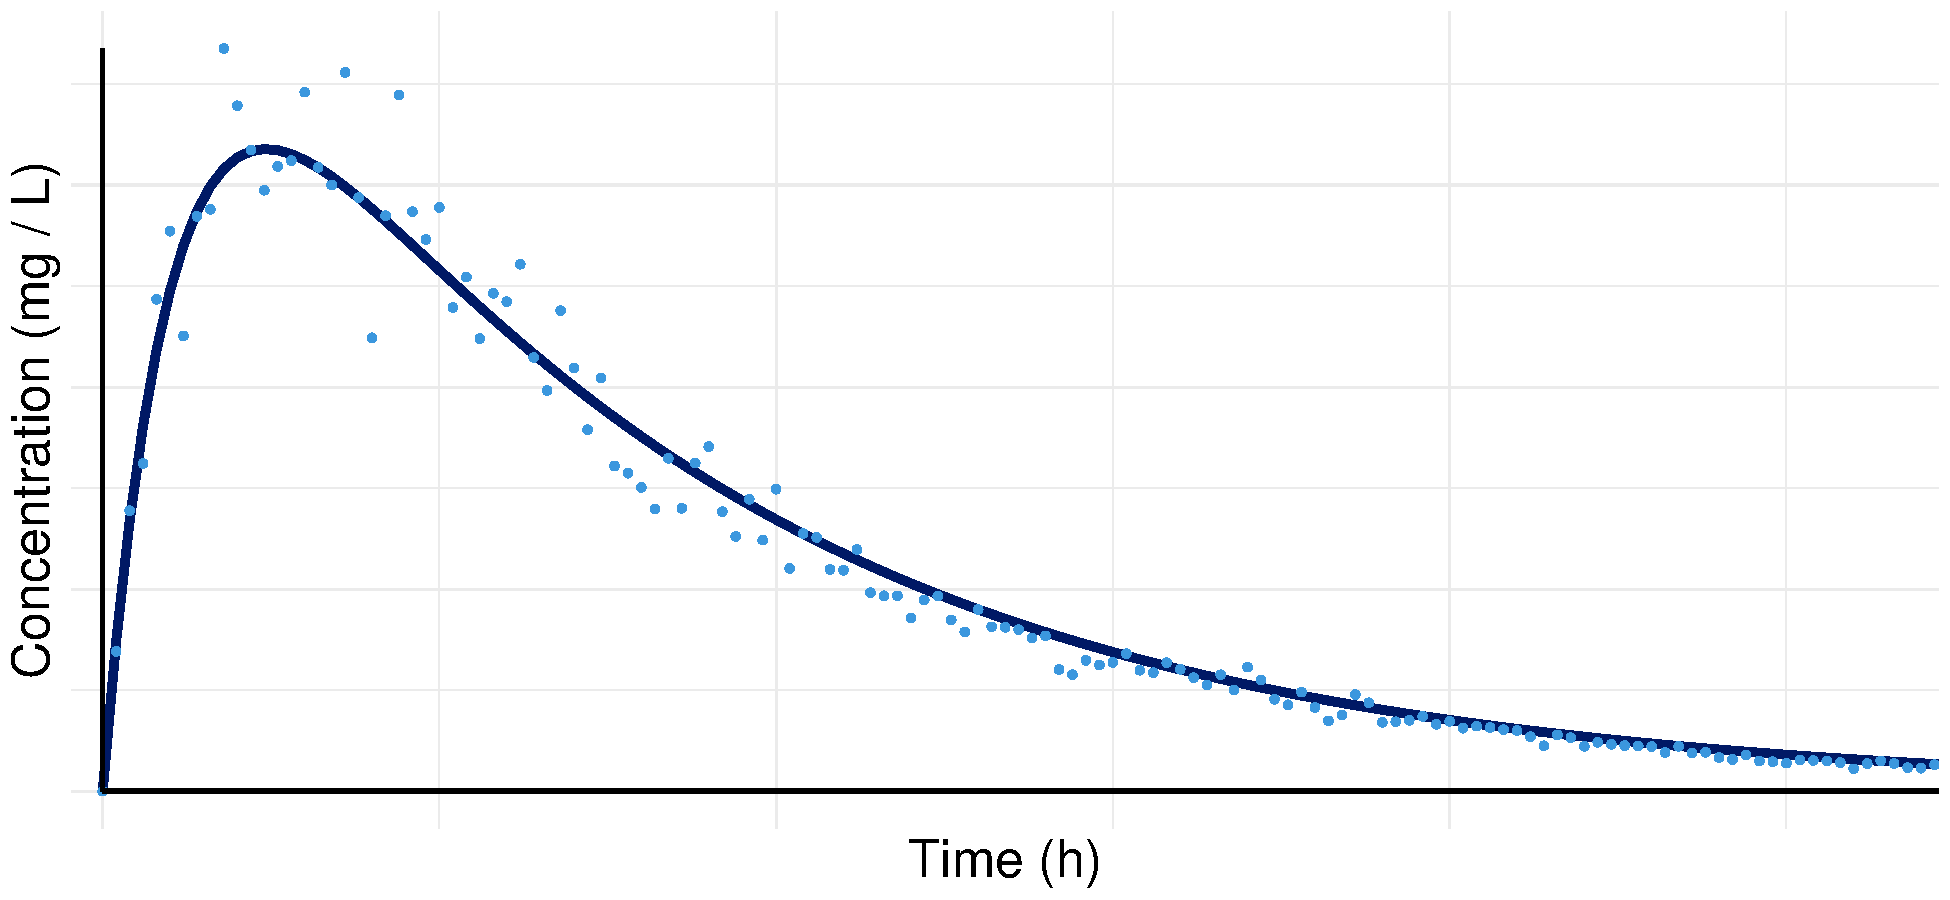
\includegraphics[width=\linewidth]{fig/img/Residual Variance Model/Concentration W. Oral Prop.pdf}
        \caption{Proportional error}
        \label{fig: Residual variance model prop}
    \end{minipage}
    \caption{Simulated concentrations from a one-compartment model with oral administration, each with different error models.}
    \label{fig: Residual variance model}
\end{figure}
% To determine which error model is most suitable, likelihood ratio tests and goodness of fit plots are used. 

\section{Estimation methods} \label{sec: Estimation methods}
% Let $g_i(\theta_i):=[g(t_{i,1}, u_i, \theta_i), g(t_{i,2}, u_i, \theta_i), \dots, g(t_{i,n_i}, u_i, \theta_i)]^\top \in \R^{n_i}$ denote the vector of mean responses for each time point measured for the $i$'th subject, and let $e_i = (e_{i,1}, \dots, e_{i,n_i})^\top \in \R^{n_i}$ denote the random errors for subject $i$.  The model specified by \eqref{eq: NLME Stage 1} and \eqref{eq: NLME Stage 2} can then be written as 
% \begin{align}
%     y_i &= g_i(\theta_i)+e_i, \quad e_i\mid \theta_i \sim (0,R_i(u_i,\theta_i,\xi)), \label{eq: stage 1 for subject i}\\
%     \theta_i &= d(a_i,\beta,\eta_i), \quad \eta_i \sim (0,\Omega)\label{eq: stage 2 for subject i},
% \end{align}
% for $i = 1,\dots,N$. The set of parameters to be estimated are $\beta \in \R^k$, $\xi=(\sigma,\psi^\top)^\top$ and $\Omega$. Here, $\beta$ and $\Omega$ are considered population parameters. To estimate these parameters, the aim is to derive the likelihood function for $\beta$, $\xi$ and $\Omega$. 

% \subsection{The Likelihood Function}
Fundamental to NLMM is the fact that \eqref{eq: NLME Stage 1} requires an assumption about the distribution of $\eta_i$, while \eqref{eq: NLME Stage 2} requires an assumption about the distribution of $y_i \mid \eta_i$, as $y_i$ depends on $\eta_i$ through $\theta_i$. Thus, the joint density of $(y_i, \eta_i)$ is given by
\begin{align*}
    p_{y,\eta}(y_i,\eta_i\mid x_i,\Theta)=p_{y\mid \eta}(y_i\mid x_i,\eta_i,\beta,\xi)p_\eta(\eta_i\mid \Omega),
\end{align*}
where $p_{y\mid  \eta}$ is the conditional density of $y_i \mid \eta_i$, and $p_\eta$ is the density of $\eta_i$. Remind that $x_i =(u_i,a_i)$ is the collection of covariates for subject $i$. The random effects serve as latent variables, implying that $\eta_i$ is unobservable. Consequently, a marginalisation w.r.t. $\eta_i$ yields the marginal distribution of $y_i$,
\begin{align}
    p_y(y_i\mid x_i,\beta,\xi)=\int_{\R^r} p_{y\mid \eta}(y_i\mid x_i,\beta,\eta_i,\xi)p_\eta(\eta_i\mid  \Omega)d\eta_i. \label{eq: marginal distribution of y_i}
\end{align}

The likelihood function for $\Theta$ can be expressed as the joint density of the observed data $y_1,y_2,\dots,y_N$ given $x_i$, which, by independence across $i$, is given by the product of the marginal densities \eqref{eq: marginal distribution of y_i},
\begin{align}
    L(\Theta\mid  y_1,y_2,\dots,y_N)&=\prod_{i=1}^N\int_{\R^r} p_{y\mid \eta}(y_i\mid x_i,\beta,\eta_i,\xi)p_\eta(\eta_i\mid  \Omega)d\eta_i.\label{eq: likelihood for parameters}
\end{align}

Under the assumption of normality, i.e. $e_i\mid \theta_i \sim N(0,R_i)$ and $\eta_i \sim N(0,\Omega)$, the densities $p_{y\mid \eta}$ and $p_{\eta}$ are given by
\begin{align*}
    p_{y\mid \eta}(y_i\mid x_i,\beta,\eta_i,\xi) &= \frac{1}{(2\pi)^{n_i/2}\mid R_i\mid ^{1/2}}\exp{\left(-\frac{1}{2}\left[y_i-g_i(\theta_i)\right]^\top R_i^{-1}\left[y_i-g_i(\theta_i)\right]\right)},\\
    p_\eta(\eta_i\mid \Omega)&=\frac{1}{(2\pi)^{r/2}\mid \Omega\mid ^{1/2}}\exp{\left(-\frac{1}{2}\eta_i^\top \Omega^{-1}\eta_i\right)}.
\end{align*}

The $N$ $r$-dimensional integrations that appear in \eqref{eq: likelihood for parameters} do not have a closed form expression -- neither when normality is assumed. This is due to the fact that the estimation of $\xi$ depends on the estimation of $\Omega$, i.e. $e_i$ is dependent on $\eta_i$, further complicated by the non-linearity of $g$ \citep[p. 254]{bonate}. Instead, the integration must be done by numeric approximation. 

% The marginal density of $y_i$ is then
% \begin{align}
%     p_y(y_i\mid x_i,\beta,\xi)=\int_{\R^r}(2\pi)^{-(n_i-r)/2}|R_i|^{-1/2}|\Omega|^{-1/2}\exp{\left(-\frac{1}{2}\Psi(\eta_i)\right)d\eta_i}, \label{eq: marginal distribution of y_i under normality}
% \end{align}
% where $\Psi(\eta_i)=\left(y_i-g_i(\theta_i)\right)^\top|R_i|^{-1}\left(y_i-g_i(\theta_i)\right)+\eta_i^\top|\Omega|^{-1}\eta_i$. 

% Insert \eqref{eq: marginal distribution of y_i under normality} as $p_y$ in \eqref{eq: likelihood for parameters} to get the likelihood function for $\beta$, $\xi$, $\Omega$ under the assumption of normality.

\subsection{First Order Conditional Estimation with Interaction}
% Kilder brugt: \cite{Almquist2015}, \cite{Bae2016}, \cite{Savic2009}, \cite{Wang2007}, \cite{Davidian1995}.
First-order conditional estimation with interaction (focei) is a general estimation method including the simpler versions; first-order conditional estimation (foce) and first-order (fo) estimation. The fo and foce methods assume an additive error model, i.e. no interaction between the residual error and the random effects, while focei can be used for any error model \citep{Bae2016}. 

Fo estimation assumes $\eta=0$, while foce and focei use conditional estimates of $\eta_i$, obtained from an inner optimisation problem. The conditional estimates of $\eta_i$ are then considered fixed when minimising the objective function in the outer optimisation problem. The estimation proceeds by iterating through the inner and outer optimisation problem for some number of iterations, or until convergence.

Generally, there are two methods to derive the focei objective function: Laplace approximation of the likelihood \eqref{eq: likelihood for parameters}, or first-order linearisation of $g(t, u_i, \theta_i)$ in \eqref{eq: NLME Stage 1} \citep[p. 161]{Bae2016}. The fo and foce methods produce the same objective function, whereas the focei method does not \citep[p. 581]{Wang2007}. 
NONMEM uses the focei objective function obtained with Laplacian approximation \citep[p. 585]{Wang2007}, and nlmixr has been shown to yield the equivalent objective function \citep{nlmixr}. For this reason, the focei objective function is derived using Laplacian approximation.

Given a complex integral, $ \int_\Omega f(x) \ dx$, with $f$ twice differentiable, and $f(x)>0 \ \forall x \in \Omega$, $f(x)$ can be expressed as $\ep{g(x)}$ with $g(x)=\log f(x)$. If $\frac{d^2 g(x)}{d x^2}\big\rvert_{x=x_0}<0$, then
\begin{align}
    \int_\Omega f(x) \ dx &\approx \int_\Omega \ep {g(x_0) +(x-x_0) \cdot\frac{d g(x)}{d x}\Big\rvert_{x=x_0} +\frac{(x-x_0)^2}{2!} \cdot \frac{d^2 g(x)}{d x^2}\Big\rvert_{x=x_0}}\ dx \label{eq: LAPL approx}
\end{align}
is the Laplacian approximation of the true integration, obtained using a second-order Taylor expansion of $g(x)$ around $x_0$. 

The Laplacian approximation \eqref{eq: LAPL approx} can be used to approximate \eqref{eq: likelihood for parameters} by letting $f(\eta_i)=p_{y\mid  \eta}\cdot p_\eta$ denote the joint density under the assumption of normality. Then
\begin{align*}
    g(\eta_i)=\log\left[\frac{1}{(2\pi)^{n_i/2}|R_i|^{1/2}}\right]-\frac{1}{2}\left[e_i^\top R_i e_i\right] + \log \left[\frac{1}{(2\pi)^{r/2}|\Omega|^{1/2}}\right] -\frac{1}{2}\left[\eta_i^\top \Omega \eta_i\right].
\end{align*}
The focei estimation method uses the Laplacian approximation with a Taylor expansion of $g(\eta_i)$ around $\eta_i^\ast = \arg \max g(\eta_i)$, i.e. the posterior mode of $g(\eta_i)$, ensuring the term of the Taylor expansion including the first derivative equals zero. Let $\Delta_i(\eta_i)=\frac{d g(\eta_i)}{d^2 \eta_i}$ denote the Hessian matrix.
% If the Taylor expansion is done around $\eta_i^\ast$, where $g'(\eta_i^\ast)=0$, it simplifies to
% \begin{align*}
%     \int_{\R^r} f(\eta_i) d\eta_i=\int_{\R^r} \exp(g(\eta_i)) d\eta_i \approx f(\eta_i^\ast) \cdot \sqrt{\frac{(2\pi)^r}{\left|-\frac{d g(\eta_i)}{d^2 \eta_i}\Big\rvert_{\eta_i=\eta_i^\ast}\right|}}.
% \end{align*}
The approximation of \eqref{eq: likelihood for parameters} is then
\begin{align}
    L(\Theta\mid  y_1,y_2,\dots,y_N)&\approx \prod_{i=1}^N\int_{\R^r} \ep { g(\eta_i^\ast) +\frac{(\eta_i-\eta_i^\ast)^2}{2!} \Delta_i(\eta_i^\ast)} \ d\eta_i \nonumber \\
    &= f(\eta_i^\ast) \cdot \sqrt{\frac{(2\pi)^r}{\left|-\Delta_i(\eta_i^\ast)\right|}},\label{eq: approx laplace likelihood}
\end{align}
where the last equality is obtained using the moment generating function of a normal random variable, with derivations provided in \cite{Wang2007} (pp. 588-589). 

The focei objective function is obtained by multiplying \eqref{eq: approx laplace likelihood} by $-2$, taking the logarithm, and using an estimate of the Hessian matrix, $\hat\Delta_i$, i.e.
\begin{align}
    O_{focei}&=\sum_{i=1}^N -2\log p_{y|\eta}(\eta_i^\ast)-2\log p_\eta(\eta_i^\ast)-\log \frac{(2\pi)^r}{\left|-\hat\Delta_i(\eta_i^\ast)\right|} \nonumber \\
    &= \sum_{i=1}^N-2\log p_{y|\eta}(\eta_i^\ast) +\log|\Omega|+{\eta_i^\ast}^\top \Omega^{-1} \eta_i^\ast +\log \left|-\hat\Delta_i(\eta_i^\ast)\right|, \label{eq: focei objective function}
\end{align}
where $\hat\Delta_i$ is approximated 
by a function of the gradient vector, ignoring the second order derivatives that are costly to compute. The explicit form of the elements of $\hat\Delta_i$ are derived in \cite{Almquist2015} (pp. 193-194). 

The foce objective function uses another estimate of $\Delta_i$, where dependence of $R_i$ on $\eta_i$ is ignored \citep[p. 194]{Almquist2015}. The fo objective function has ${\eta_i^\ast}^\top \Omega^{-1} \eta_i^\ast=0$, but includes an extra term arising from the first derivative term in the Taylor expansion as $\frac{dg(\eta_i)}{d\eta_i}\rvert_{\eta_i=0}=0$ is not ensured. The explicit form of the fo and foce objective functions are provided in \cite{Wang2007} (pp. 580-581). 

In both NONMEM and nlmixr, the constant $n_i \log 2\pi$ in $-2\log p_{y|\eta}$ is not included in the focei objective function \eqref{eq: focei objective function} \citep[p. 581]{Wang2007, nlmixr}.

In the inner optimisation problem, the current estimate of $\Theta$ is fixed to solve $\eta_i^\ast = \arg \max g(\eta_i)$. The obtained estimate $\eta_i^\ast$ is then fixed in \eqref{eq: focei objective function} to solve the outer optimisation problem, i.e. $\hat{\Theta}=\arg_{\Theta} \min O_{focei}$, and this new estimate is then fixed to obtain new estimates of $\eta_i^\ast$. The estimation method is thus based on two optimization procedures, both of which can be specified within nlmixr.

The final estimates of $\hat{\eta_i}$ have an empirical Bayes interpretation \citep[p. 170]{Davidian1995}, that can be used to determine shrinkage of the subject specific parameters. 

The default inner optimisation algorithm used in nlmixr is a Quasi-Newton Broyden–Fletcher–Goldfarb–Shanno (BFGS) algorithm without constraints. The package used is 'n1qn1' which is an R port of the optimisation procedure in scilab \citep{n1qn1}. The default outer optimisation problem used in nlmixr is an unconstrained and bounds-constrained quasi-Newton method optimizer from base \textit{R} called 'nlminb' \citep{R-base}. In NONMEM, proprietary closed source optimisation algorithms are used \cite{githubEstimationProceeding}. Differences in final estimates from nlmixr vs. NONMEM can therefore be due to differences in estimation methods.

% \subsection{First-Order Estimation}
% % FO: No (small) IIV, assumes additive error model. No inner optimisation problem. FOCE: Additive error model. FOCE-i: Proportional (or combined) error model. Generally two methods: Laplacian approximation and linearisation. These two methods yield equivalent objective functions for FO and FOCE, however not for FOCE-i. NONMEM uses the Laplacian approximation. (WANG). What does nlmixr use? FOCE-i, innerOpt = c("n1qn1", "BFGS"), outerOpt = c("nlminb", "bobyqa", "lbfgsb3c", "L-BFGS-B", "mma", "lbfgsbLG", "slsqp",
% % "Rvmmin").
% The first-order (FO) method models a linear approximation of \eqref{eq: likelihood for parameters} using a Taylor expansion around $\eta_i=0$. The method uses a Cholesky decomposition of $R_i$, 

% Since $R_i(u_i,\theta_i,\xi)$ is diagonal, its Cholesky decomposition is simply $R_i=R_i^{1/2}R_i^{1/2}$. Let $\epsilon_i \sim (0,I_{n_i})$ and write the residual error as $e_i=R_i^{1/2}\epsilon_i$. This rewriting is justified since $\Ex{e_i \mid \theta}=\Ex{R_i^{1/2}\epsilon_i}=0$ and $\Var{e_i \mid \theta_i}=\Var{R_i^{1/2}\epsilon_i \mid \theta_i }=R_i^{1/2}\Var{\epsilon_i}R_i^{1/2}=R_i$. The model \eqref{eq: NLME Stage 1} can then be written as 
% \begin{align*}
%     y_i &= g_i(\theta_i) + R_i^{1/2}(u_i,\theta_i,\xi)\epsilon_i \\
%     &= g_i(d(a_i,\beta,\eta_i)) + R_i^{1/2}(u_i,d(a_i,\beta,\eta_i),\xi)\epsilon_i, \quad \epsilon_i \sim N(0,I_{n_i}),
% \end{align*}
% where the dependence on the $\eta_i$'s are written explicitly.

% The idea is then to use a Taylor expansion around $\eta_i=0$. This yields the first order approximation of $y_i$,
% \begin{align}
%     y_i \approx g_i(d(a_i,\beta,0)) + R_i^{1/2}(u_i,d(a_i,\beta,0),\xi)\epsilon_i + (derivA + derivB)\eta_i. \label{eq: FO approx}
% \end{align}
% The last term is omitted, as misspecification of second order moments is not as crucial as for first order moments (kilde). Denote derivA $:= Z_i(\beta,0)$ and $e_i^{\ast}:= R_i^{1/2}(u_i,d(a_i,\beta,0),\xi)\epsilon_i$ to get the representation 
% \begin{align*}
%        y_i \approx g_i(d(a_i,\beta,0)) + Z_i(\beta,0)\eta_i + e_i^{\ast}. 
% \end{align*}
% The approximated marginal first and second moment of $y_i$ is then
% \begin{align*}
%     \Ex{y_i} &\approx g_i(d(a_i,\beta,0)),\\
%     \Var{y_i} &\approx \Var{Z_i(\beta,0)\eta_i} + \Var{e_i^{\ast}}\\
%     &= Z_i(\beta,0)\Var{\eta_i}Z_i^{\top}(\beta,0) + R_i^{1/2}(u_i,d(a_i,\beta,0),\xi)\Var{\epsilon_i}R_i^{1/2}(u_i,d(a_i,\beta,0),\xi)\\
%     &=  Z_i(\beta,0)\Omega Z_i^{\top}(\beta,0) + R_i^{1/2}(u_i,d(a_i,\beta,0),\xi)\\
%     &=:V_i(\beta,0,\xi,\Omega).
% \end{align*}
% Under the assumption of normality, i.e. $e_i \sim N(0,V_i(\beta,0,\xi,\Omega))$ and $\eta_i \sim N(0,\Omega)$, the marginal density of $y_i$ is
% \begin{align*}
%         p_{y}(y_i\mid x_i,\beta,\xi,D) &= \frac{1}{(2\pi)^{n_i/2}\mid V_i(\cdot)\mid ^{1/2}}\exp{\left(-\frac{1}{2}Q(\cdot)\right)},
% \end{align*}
% where $Q(\cdot)=\left[y_i-g_i(d(a_i,\beta,0))-Z_i(\beta,0)\eta_i\right]^\top V_i^{-1}(\cdot)\left[y_i-g_i(d(a_i,\beta,0))-Z_i(\beta,0)\eta_i\right]$. The likelihood is then given by
% \begin{align*}
%     L(\beta,\xi,\Omega \mid y_1,\dots,y_N)=\prod_{i=1}^N p_{y}(y_i\mid x_i,\beta,\xi,D),
% \end{align*}
% and thus the log likelihood is
% \begin{align*}
%     l(\beta,\xi,\Omega \mid y_1,\dots,y_N)=\sum_{i=1}^N p_{y}(y_i\mid x_i,\beta,\xi,D) \propto \sum_{i=1}^N-\frac{1}{2}\log|V_i(\cdot)|-\frac{1}{2}Q.
% \end{align*}
% Multiply this with $-2$ to get the objective function to be minimised,
% \begin{align*}
% L_{FO}=\sum_{i=1}^N\log|V_i(\cdot)|+Q(\cdot),
% \end{align*}
% This is therefore equal to twice the negative normal log likelihood under assumption \eqref{eq: FO approx}.

% Minimisation of the objective function is done using different optimisation methods.

% \section{yap}
% Fiddler skrev i august 24', at NONMEM bruger "proprietary closed source optimization algorithm" til at optimere likelihood. link \url{https://github.com/nlmixr2/nlmixr2/discussions/257}, så...? Generelt har nlmixr flere optimeringsmuligheder.

% The assumptions are
% \begin{align*}
%     \Ex{e_i \mid  \theta_i}&=0,\\
%     \Var{e_i\mid \theta_i}&=R_i(u_i,\theta_i,\xi), \quad \xi=(\sigma,\psi^\top)^\top.
% \end{align*}

% The integral in \eqref{eq: marginal distribution of y_i} cannot be analytically expressed. Instead, the integration must be done by numeric approximation. The integral is intractable since the estimate of $\xi$ depends on the estimate of $\Omega$, i.e. estimation of $e_i$ depends on the estimation of $\eta_i$. Moreover, the non-linearity of $g(\cdot)$ further complicates the evaluation of the integral.


% => Påbegynd estimationsmetoder


% Options in nlmixr
% \begin{itemize}
%     \item FO: first order approximation - algorithm which transforms the NLME model into a linear ME model through a first-order Taylor approximation around the vector $\eta =0$; the model is then estimated based on the linear approximaiton to the non-linear model.
%     \item FOCE: first order conditional estimation (see Wang 2009) - first order taylor approximation around the posterior mode of $\eta$, thus it depends on a conditional estimate of $\eta$
%     \item FOCE-I: first order conditional estimation with interaction - same as foce, but it also accounts for interaction between $\eta$ and $e$ (e.g. proportional random error model). This method not useful when residual variance is large or $n_i$'s are small, neither for homoscedastic error models.

%     \item FO-I: first order with interaction

%     \item SAEM: stochastic approximation expectation-maximization
% \end{itemize}
% Andre metoder er til population-only data og ikke mixed effects modeller.


% NONMEM 
% \begin{itemize}
%     \item First Order Conditional Estimation (FOCE)
%     \item Laplace Conditional Estimation
%     \item Iterative Two Stage (ITS) 
%     \item Importance Sampling Expectation-Maximization (IMP)
%     \item Stochastic Approximation Expectation-Maximization (SAEM)
%     \item Markov-Chain Monte Carlo Bayesian Analysis (BAYES, NUTS) 
% \end{itemize}


\subsection{Stochastic Approximation Expectation-Maximization}
The Expectation-Maximaization (EM) algorithm will be explained. The algorithm is useful for maximum likelihood estimation for parameters when latent variables are present. When estimating PK models with NLMEM the laten variables are the subject specific parameters. 

The log likelihood of the concentration is
\begin{align*}
    \ell (\beta) = \log p(y;\beta) = \log \int p(y,\theta;\beta) dz
\end{align*}
where $\beta = (\beta_1, \dots, \beta_k)^{\top}$ is the parameters we wish to maximize, while $p(y,\theta)$ is the joint distribution of the concentration and the subject-specific parameters. As $\theta$ is unobserved the likelihood marginalize over $\theta$. Due to the marginalization, the likelihood can be difficult to obtain analytically. Instead the EM-algorithm can be used. 

To understand how the EM-algorithm works, a Q-function will be derived from the log-likelihood
\begin{align*}
    \ell (\beta; y) &= \log \int p(y,\theta | \beta)\\
    &= \log \int \frac{p(y,\theta|\beta)}{p(\theta|y,\hat{\beta}^{(t)})}p(\theta|y,\hat{\beta}^{(t)}) d\theta\\
    &=\log \mathbb{E}_{\theta| y, \hat{\beta}^{(t)}}\left[{\frac{p(y,\theta|\beta)}{p(\theta|y,\hat{\beta}^{(t)})}}\right]\\
    &\geq \mathbb{E}_{y,\theta| y, \hat{\beta}^{(t)}}\left[{\log\frac{p(\theta|\beta)}{p(\theta|y,\hat{\beta}^{(t)})}}\right] \\
    &=\mathbb{E}_{\theta| y, \hat{\beta}^{(t)}}\left[\log p(y,\theta| \beta) \right] - \mathbb{E}_{\theta| y, \hat{\beta}^{(t)}}\left[\log p(\theta| y, \hat{\beta}^{(t)}) \right]\\
    &= Q(\beta | \hat{\beta}^{(t)}) - \mathbb{E}_{\theta| y, \hat{\beta}^{(t)}}\left[\log p(\theta| y, \hat{\beta}^{(t)}) \right] = q(\beta | \hat{\beta}^{(t)}).
\end{align*}
The inequality in the derivation follows from Jensen's inequality. As the logarithm is a concave function the inequality becomes an equality for $\beta = \hat{\beta}^{(t)}$, thus
\begin{align*}
    \ell(\beta; y) \geq q(\beta| \hat{\beta}^{(t)})
\end{align*}
for all $\beta$, and is an equality for $\beta = \hat{\beta}^{(t)}$. 

An increase in $q(\beta | \hat{\beta}^{(t)})$ increases $\ell(\beta ; y)$ by at least as much, since
\begin{align*}
    \ell(\beta) - \ell(\hat{\beta}^{(t)}) \geq q(\beta | \hat{\beta}^{(t)}) - q(\hat{\beta}^{(t)} | \hat{\beta}^{(t)}).
\end{align*}
Therefore it is of interest to maximize $q(\beta | \hat{\beta}^{(t)})$ over $\beta$, which is equivalent to maximizing $Q(\beta | \hat{\beta}^{(t)})$.

To summarize, the q-function is a convex function that is equal to the log-likelihood function in exactly one point. Also the q-function is bounded by the log-likelihood function and an increase in the q-function yield an increase in the log likelihood function. Thus, the EM-algorithm is outlined as
\begin{itemize}
    \item Initialize the parameter estimates: $\hat{\beta}^{(0)}$
    \item E-step: Compute the Q-function
    \begin{align*}
        Q(\beta | \hat{\beta}^{(t)}) = \mathbb{E}_{\theta | y, \hat{\beta}^{(t)}} \left[\log p(\theta; \beta) \right]
    \end{align*}
    \item M-step: Maximize the Q-function to update the parameters
    \begin{align*}
        \hat{\beta}^{(t+1)} = \operatorname*{argmin}_\beta Q(\beta | \hat{\beta}^{(t)})
    \end{align*}
\end{itemize} 
\citep{columbia}.
In the cases where the regression function $g(\cdot)$ does not linearly depend on the random effects, the E-step cannot be performed i a closed-form. Instead replacing the usual
E-step of EM by a stochastic procedure

\begin{itemize}
    \item Simulation-step: draw $\theta^{(k)}$ from the conditional distribution $p(\cdot|y)$
    \item Stochastic approximation: update $ Q(\beta | \hat{\beta}^{(t)})$ s.t. it becomes $ Q(\beta | \hat{\beta}^{(t)})= Q(\beta | \hat{\beta}^{(t-1)})+\gamma_t(\log p(\theta; y, \beta)-Q(\beta | \hat{\beta}^{(t-1)}))$
    \item Maximization-step: Update $\hat{\beta}^{(t+1)}$ s.t. $\hat{\beta}^{(t+1)} = \operatorname*{argmin}_\beta Q(\beta | \hat{\beta}^{(t)})$
\end{itemize}
During the simulation step, the latent variables are generated in each iteration using a Markov Chain Monte Carlo method based on the current conditional distribution of the individual parameters. 

In the stochastic approximation step, the term $\gamma_t$ represents the "learning rate," which regulates the convergence of the SAEM algorithm. This learning rate should be a decreasing sequence that converge to $0$ at a rate slower than $1$ in relation to the number of iterations. \citep{Comets2017}



A comparison of the FOCEI and SAEM can be found in \citep{Schoemaker2019}. In the conclusion Schoemaker states: "The results indicate that output is closely comparable
across estimation algorithms"

Bonate states: "If FOCE
fails, then a stochastic estimation algorithm like SAEM or
importance sampling can be tried" \citep[p.304]{bonate}


\section{Diagnostics - Plots explained}
\begin{figure}
    \centering
    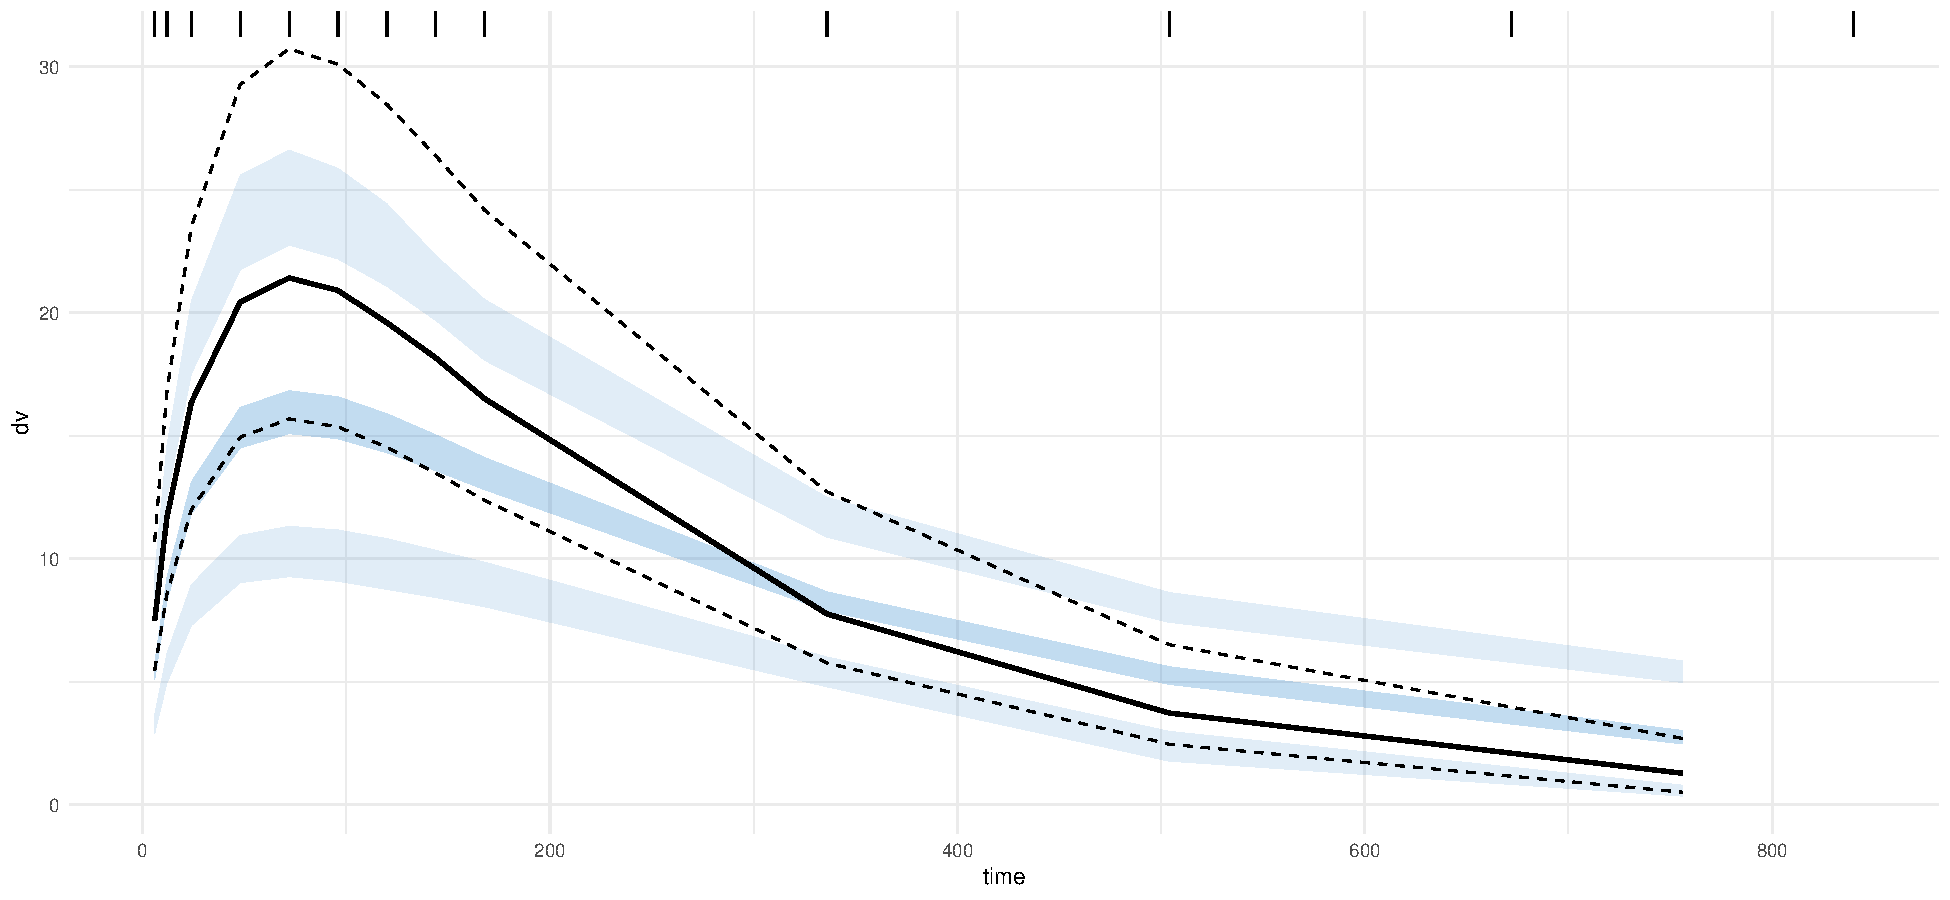
\includegraphics[width=0.9\linewidth]{fig/img/Xpose/vpcPlot.pdf}
    \caption{Enter Caption}
    \label{Fig: VPC}
\end{figure}
A VPC plot is seen in Figure \ref{Fig: VPC}. The plot is constructed from stochastic simulations, usually $n \geq 1000$, from the fitted model. From this simulation, percentiles are plotted versus time. 

Comparing the percentiles from the simulated data with the percentiles from the observed data to aid comparison of the prediction with the observed data. 

When dealing with sparse data less extreme percentiles such as the 75th and 25th percentiles may be more appropriate, as the stochastic component can yield more extreme quantiles. 

In the plot, the light blue are the simulated percentiles, while the darker blue is the simulated median. The dashed lines are the percentiles for the observed data, while the solid line is the median for the observed data. 

As $n \geq 1000$ we get at least $1000$ simulated datasets where the PI are computed. For each simulated dataset, we compute the desired quantiles (for example, the $2.5$th and $97.5$th percentiles) of the simulated observations at each time point. These quantiles will form the lower and upper bounds of the predictive intervals.

A good fit is when the observed median and confidence intervals aligns with the prediction interval and the predicted median. 
% https://www.page-meeting.org/?abstract=1434#:~:text=In%20a%20typical%20VPC%2C%20the,time%20since%20start%20of%20treatment.

\begin{figure}[htbp]
    \centering
    % First 2x2 grid
    \begin{subfigure}[b]{0.45\linewidth}
        \centering
        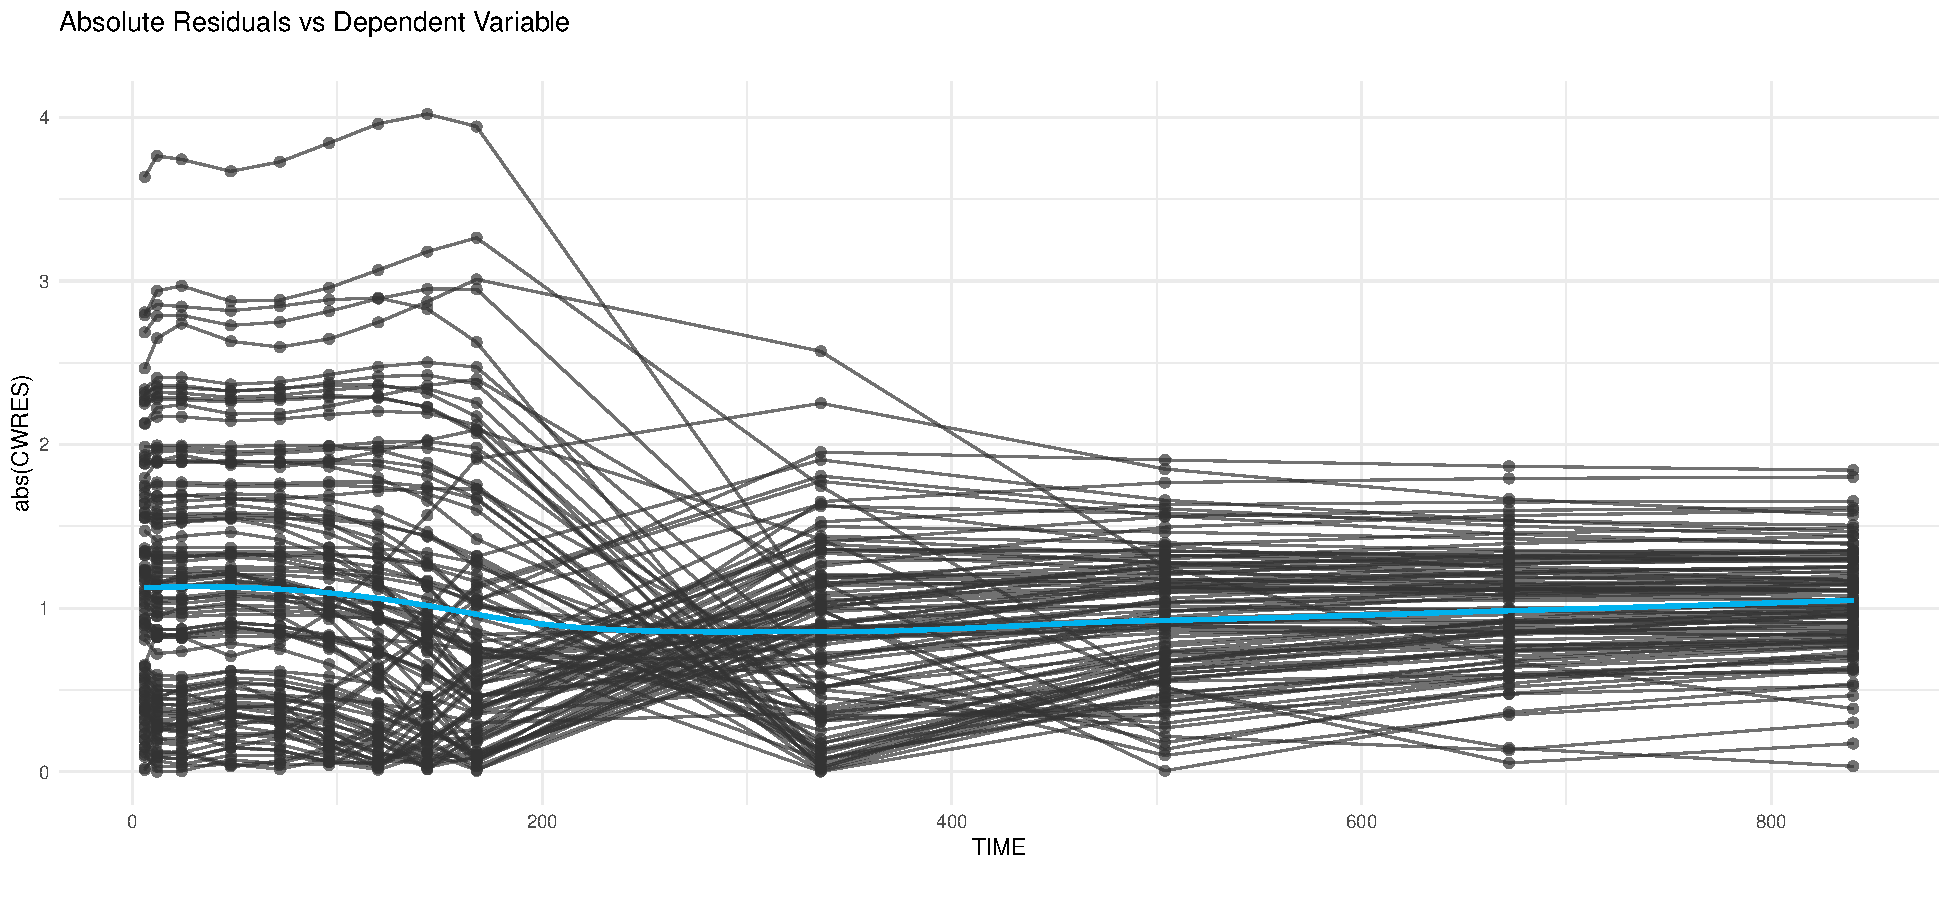
\includegraphics[width=\linewidth]{fig/img/Xpose/absval_res_vs_idv.pdf}
        \caption{absval\_res\_vs\_idv}
        \label{fig:absval_res_vs_idv}
    \end{subfigure}
    \hfill
    \begin{subfigure}[b]{0.45\linewidth}
        \centering
        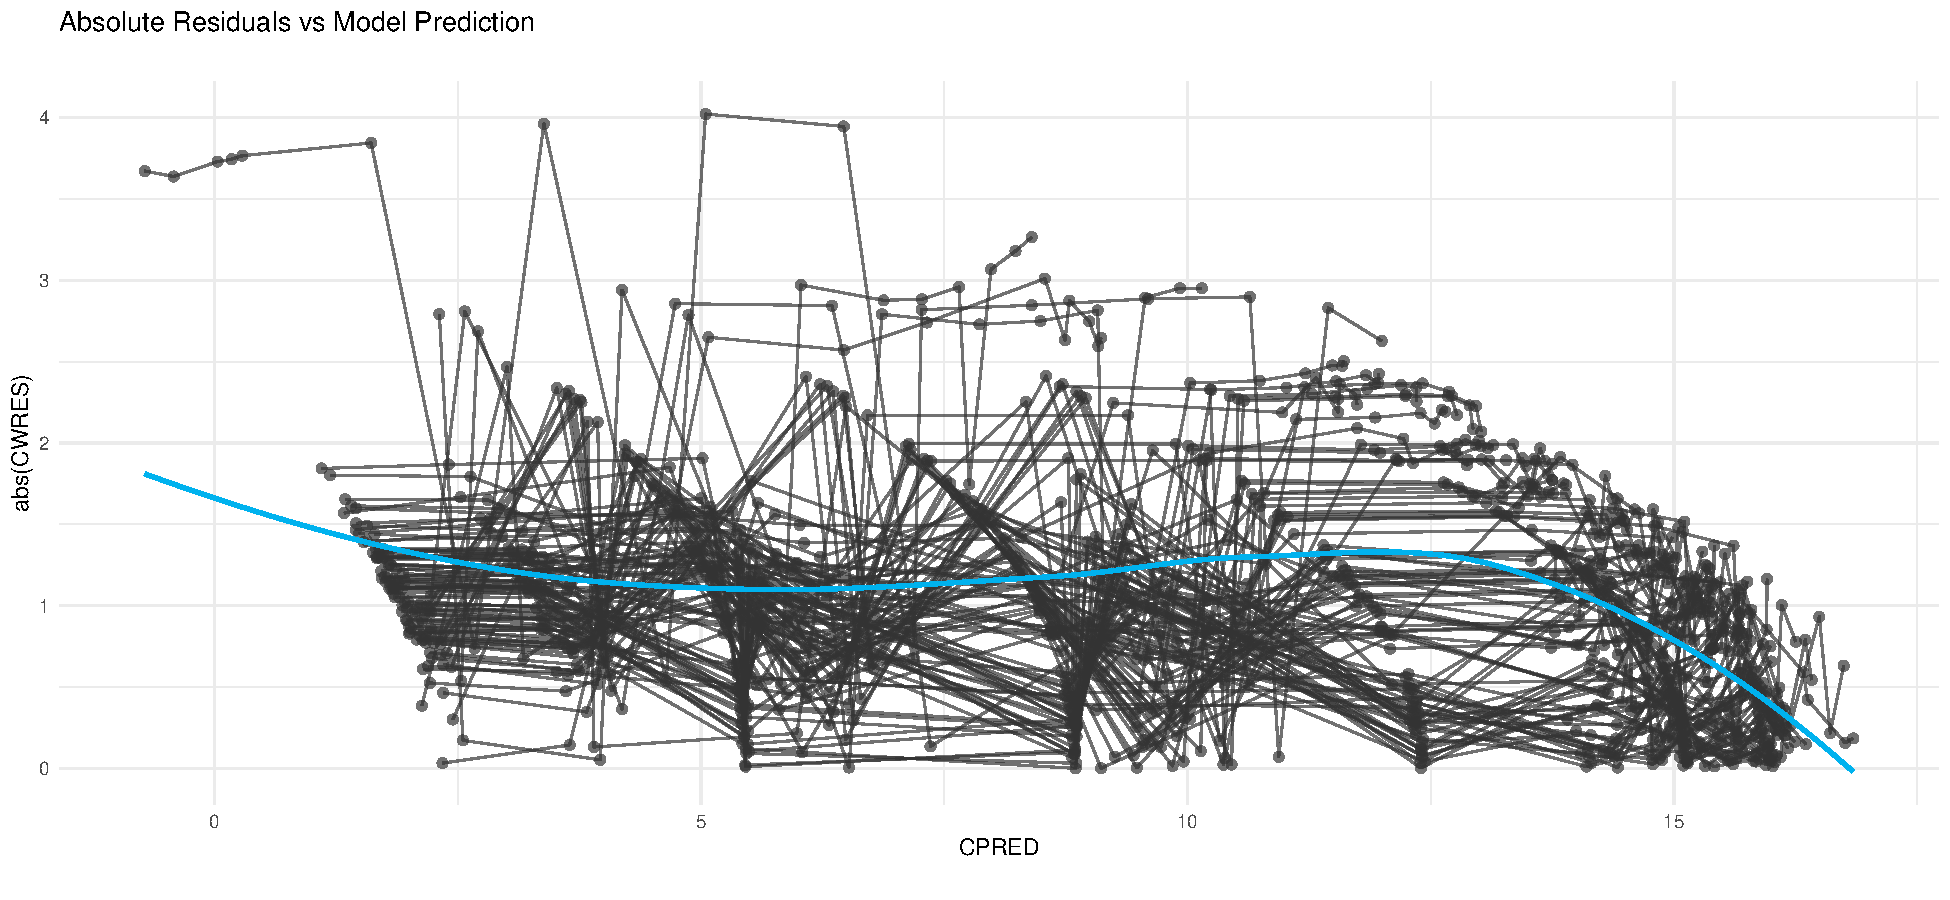
\includegraphics[width=\linewidth]{fig/img/Xpose/absval_res_vs_pred.pdf}
        \caption{absval\_res\_vs\_pred}
        \label{fig:absval_res_vs_pred}
    \end{subfigure}
    
    \vspace{1em} % Adjust vertical space between rows

    \begin{subfigure}[b]{0.45\linewidth}
        \centering
        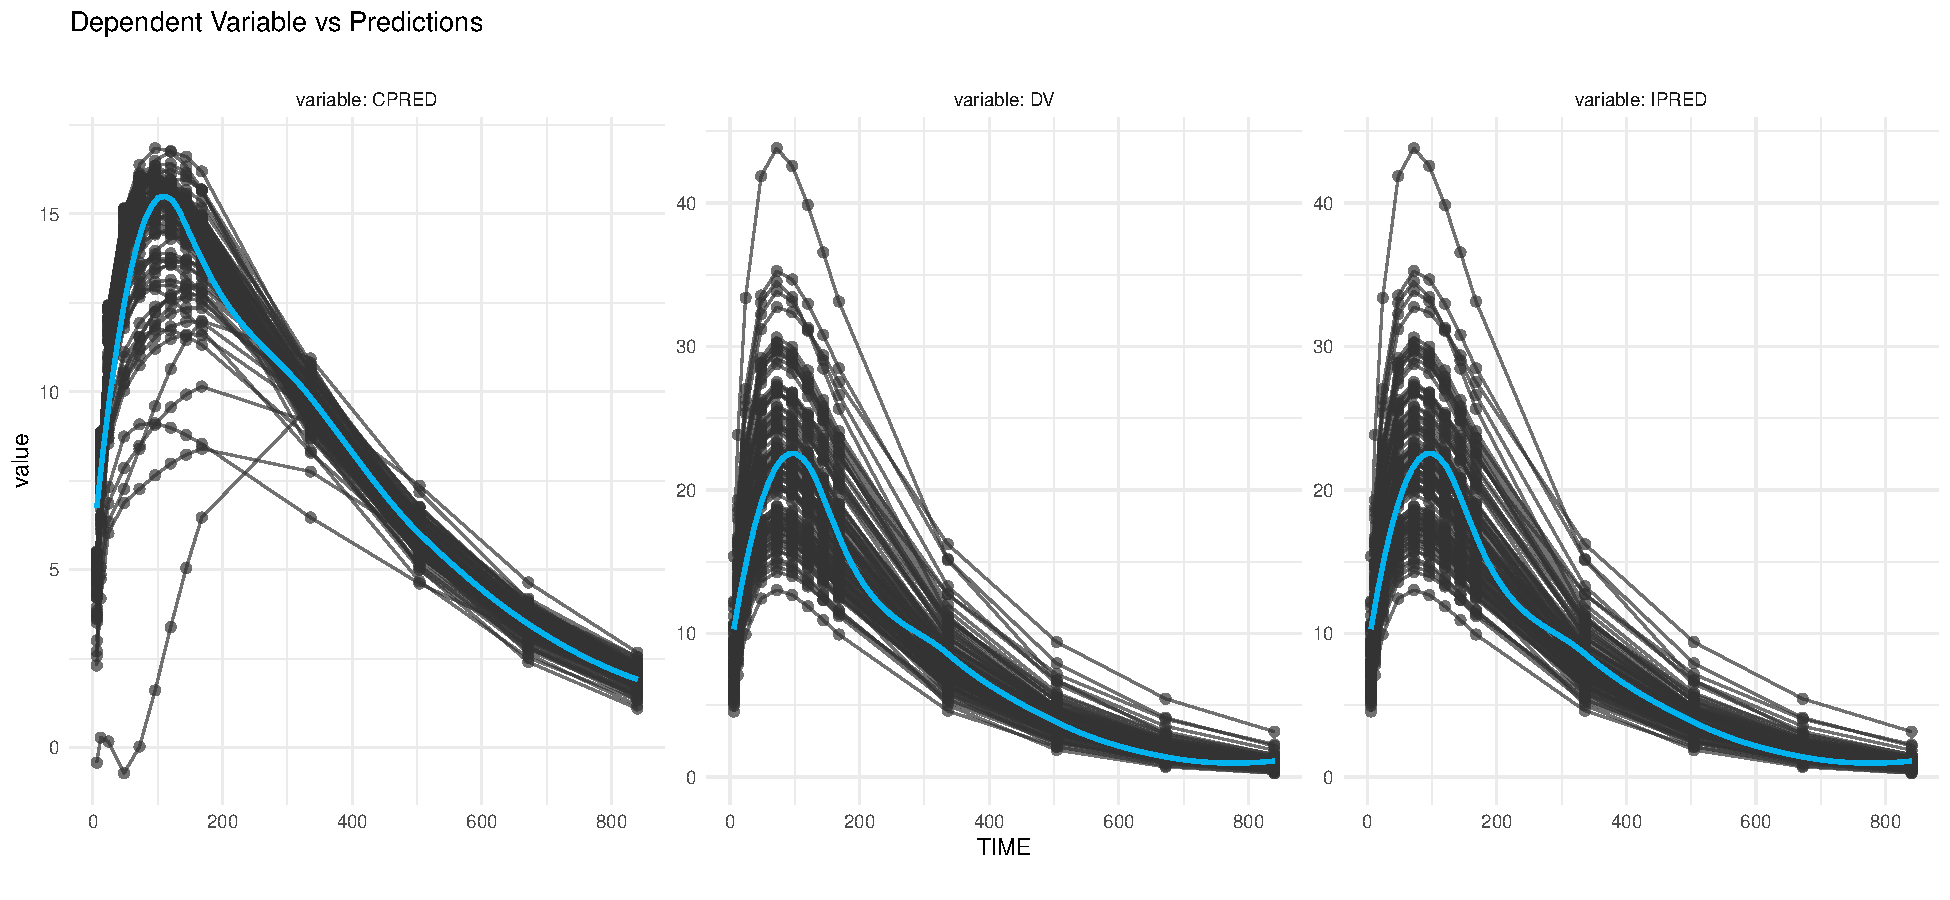
\includegraphics[width=\linewidth]{fig/img/Xpose/dv_preds_vs_idv.pdf}
        \caption{dv\_preds\_vs\_idv}
        \label{fig:dv_preds_vs_idv}
    \end{subfigure}
    \hfill
    \begin{subfigure}[b]{0.45\linewidth}
        \centering
        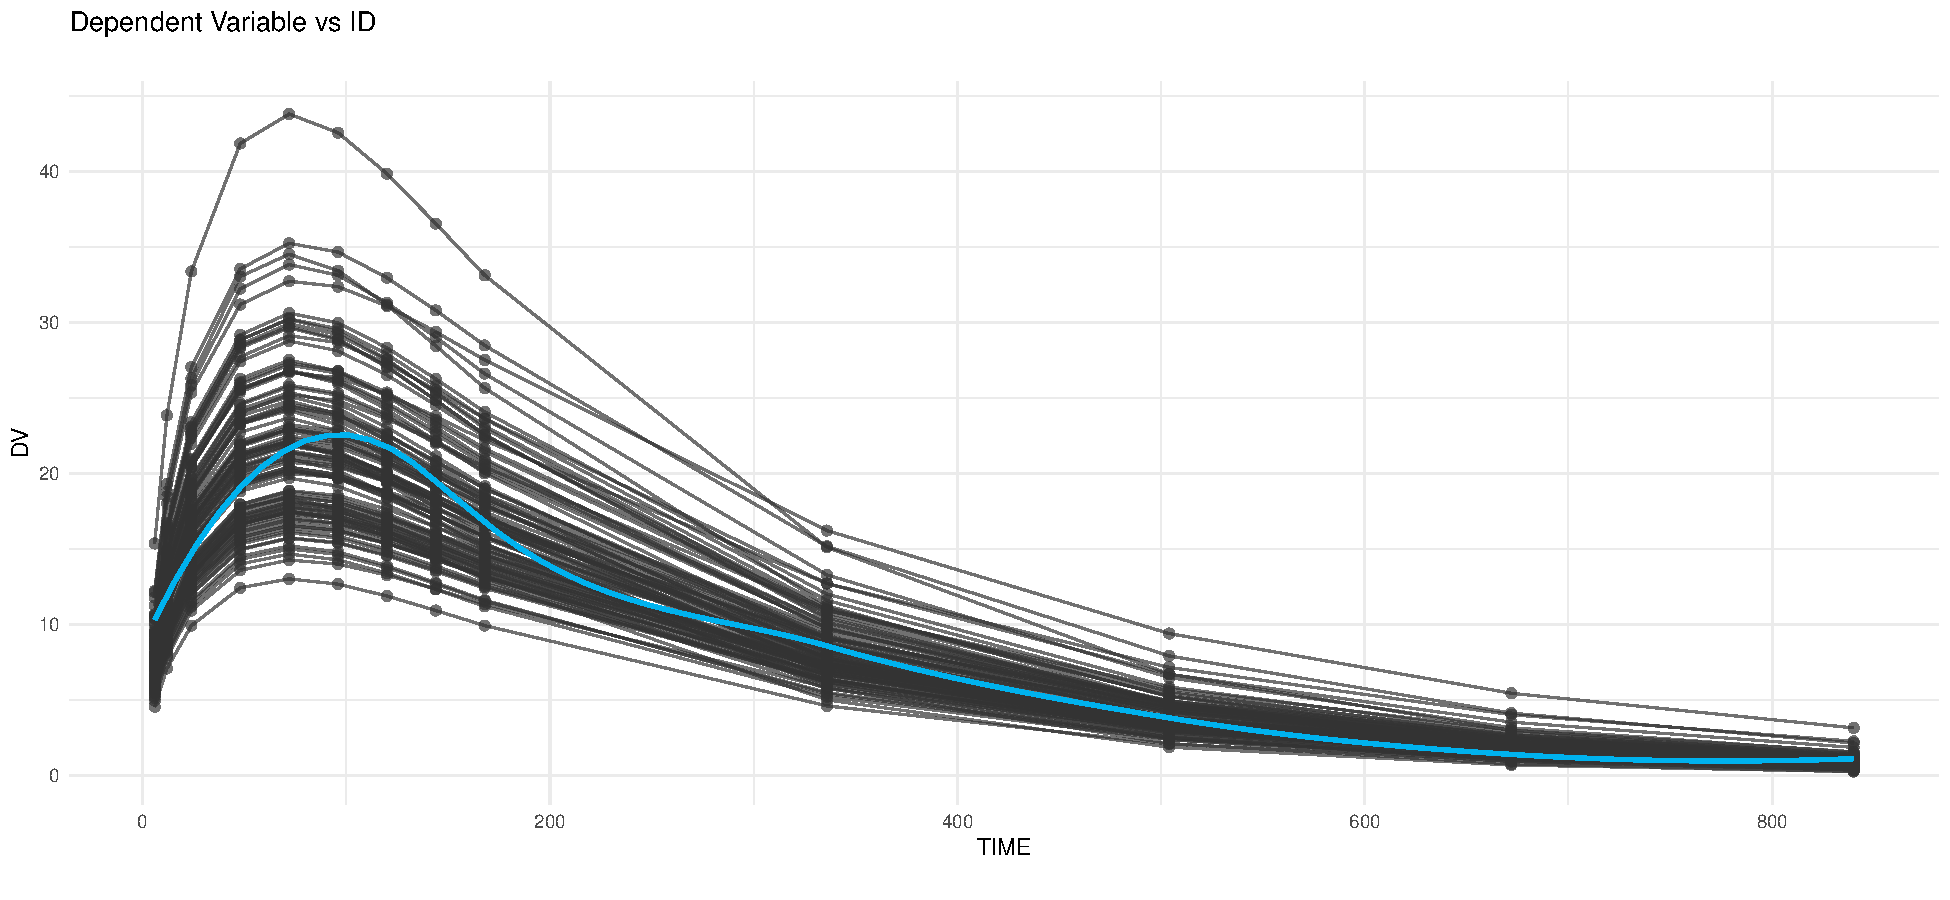
\includegraphics[width=\linewidth]{fig/img/Xpose/dv_vs_idv.pdf}
        \caption{dv\_vs\_idv}
        \label{fig:dv_vs_idv}
    \end{subfigure}

    \vspace{1em}

    % Second 2x2 grid
    \begin{subfigure}[b]{0.45\linewidth}
        \centering
        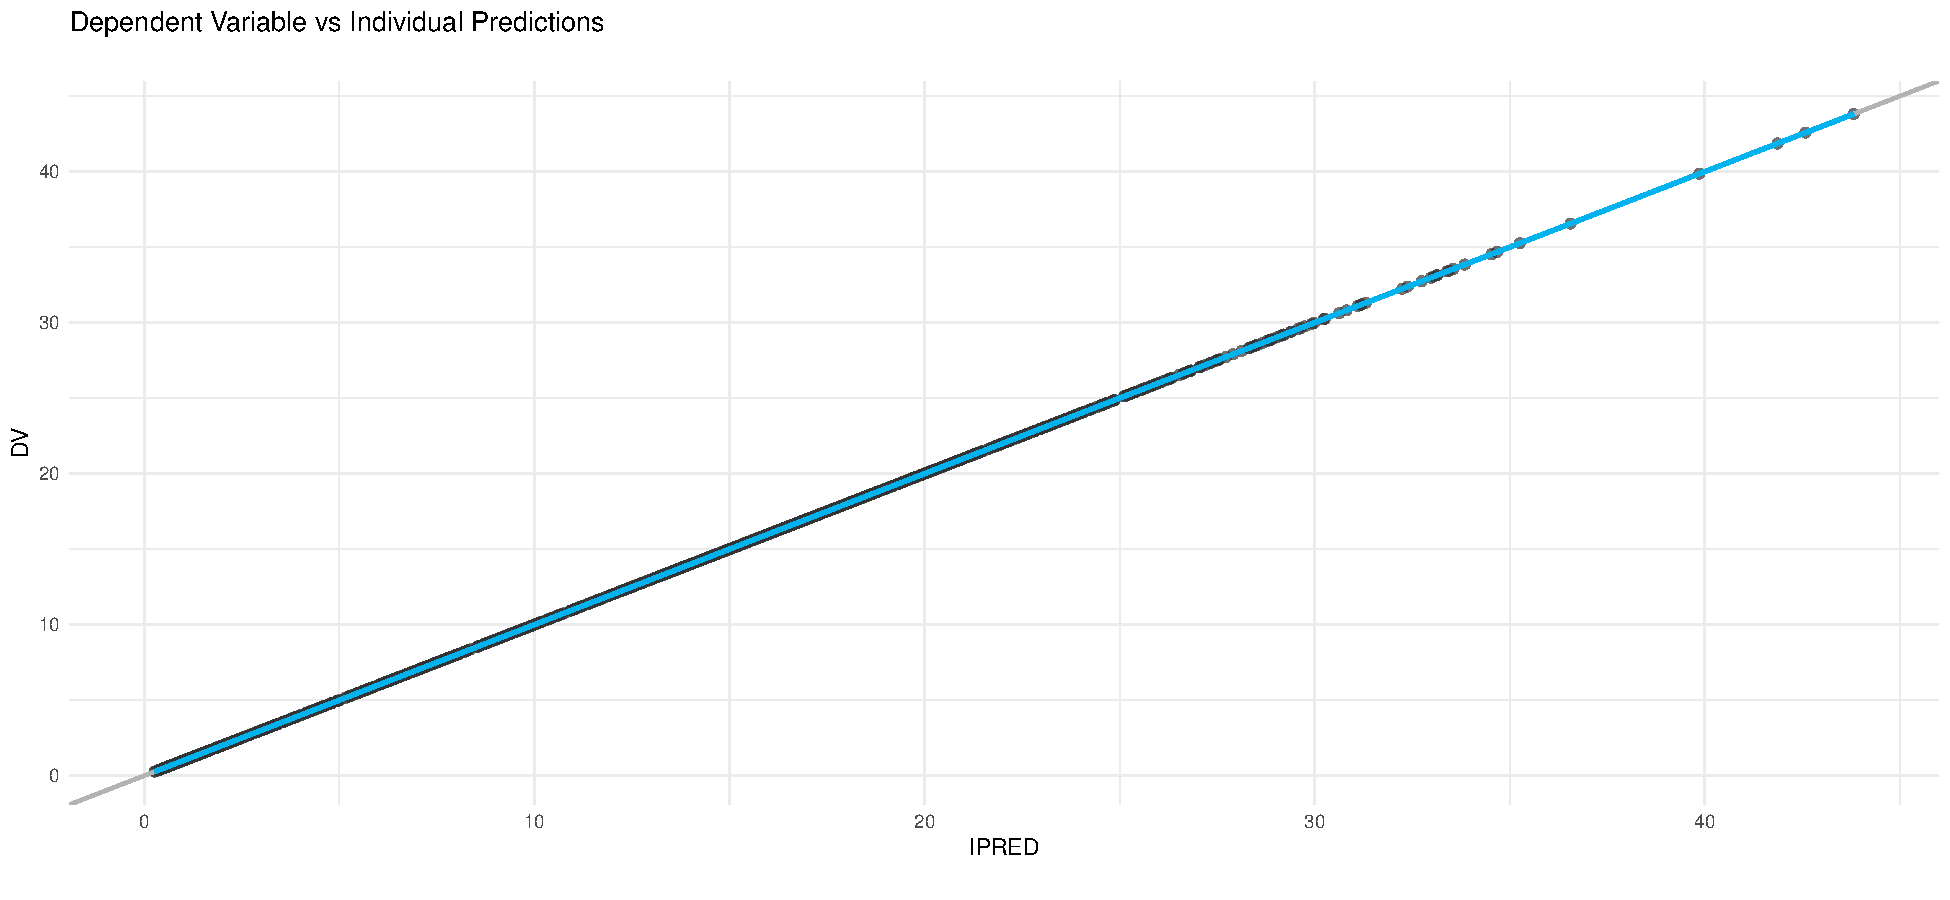
\includegraphics[width=\linewidth]{fig/img/Xpose/dv_vs_ipred.pdf}
        \caption{dv\_vs\_ipred}
        \label{fig:dv_vs_ipred}
    \end{subfigure}
    \hfill
    \begin{subfigure}[b]{0.45\linewidth}
        \centering
        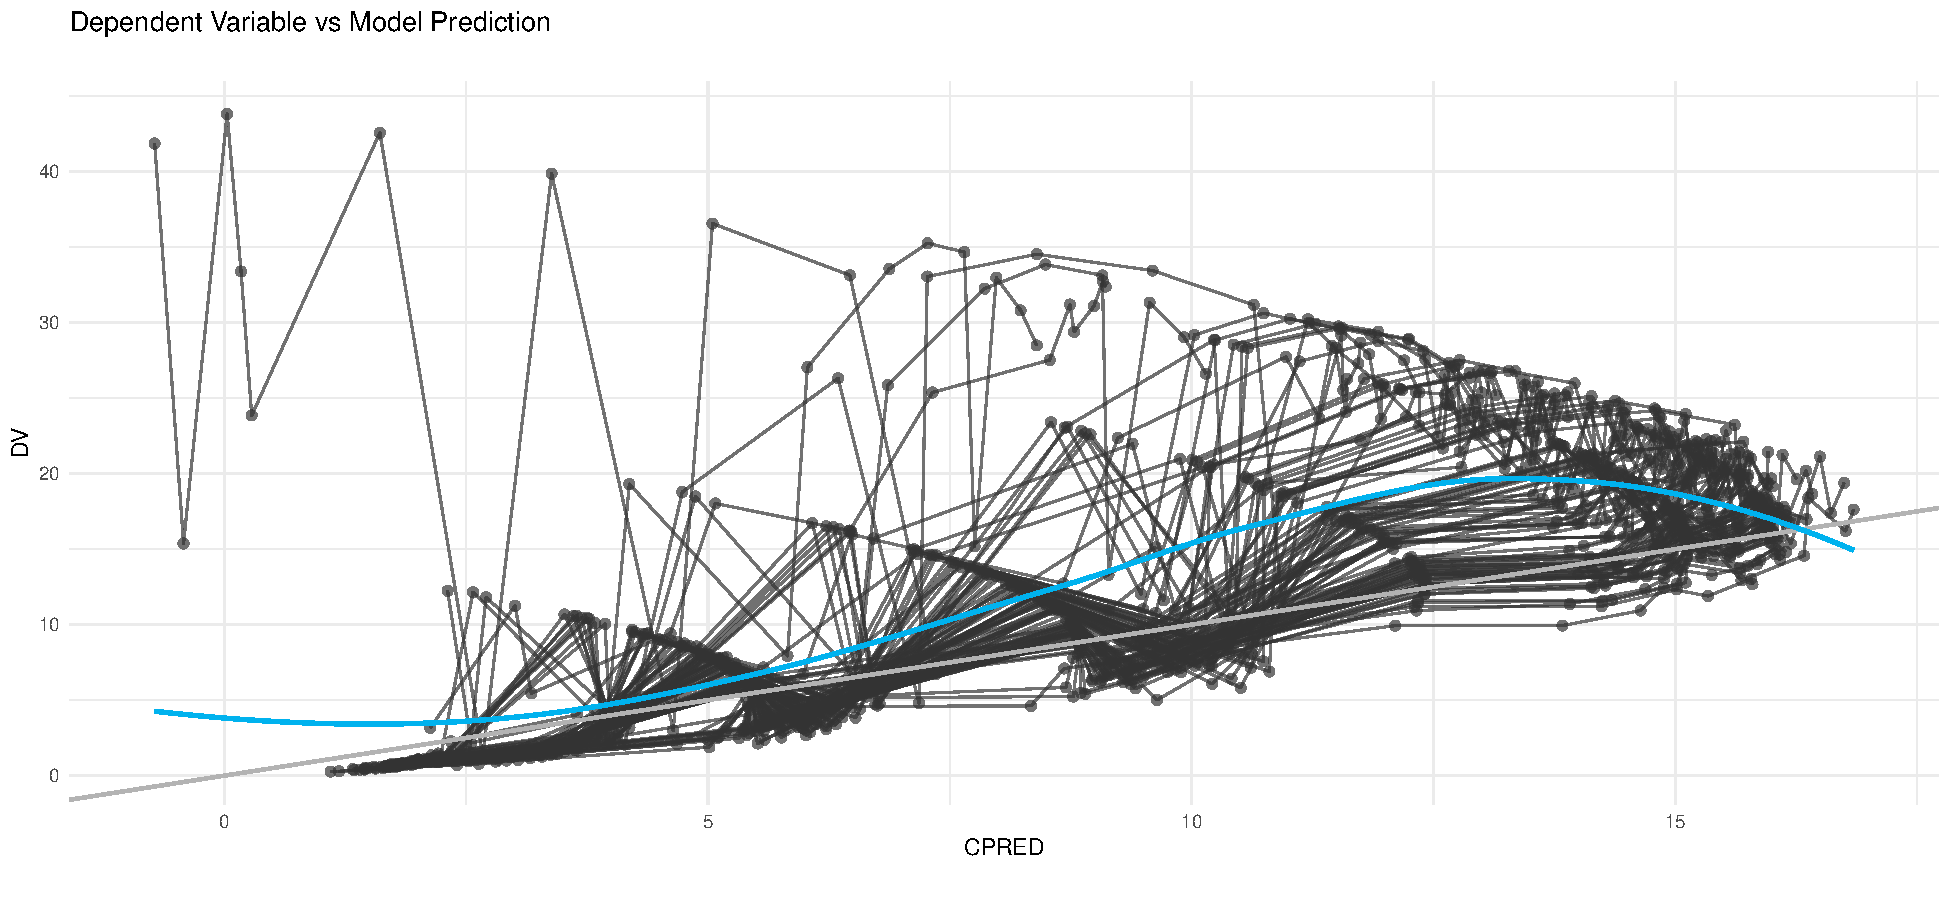
\includegraphics[width=\linewidth]{fig/img/Xpose/dv_vs_pred.pdf}
        \caption{dv\_vs\_pred}
        \label{fig:dv_vs_pred}
    \end{subfigure}

    \vspace{1em}

    % Third 2x2 grid
    \begin{subfigure}[b]{0.45\linewidth}
        \centering
        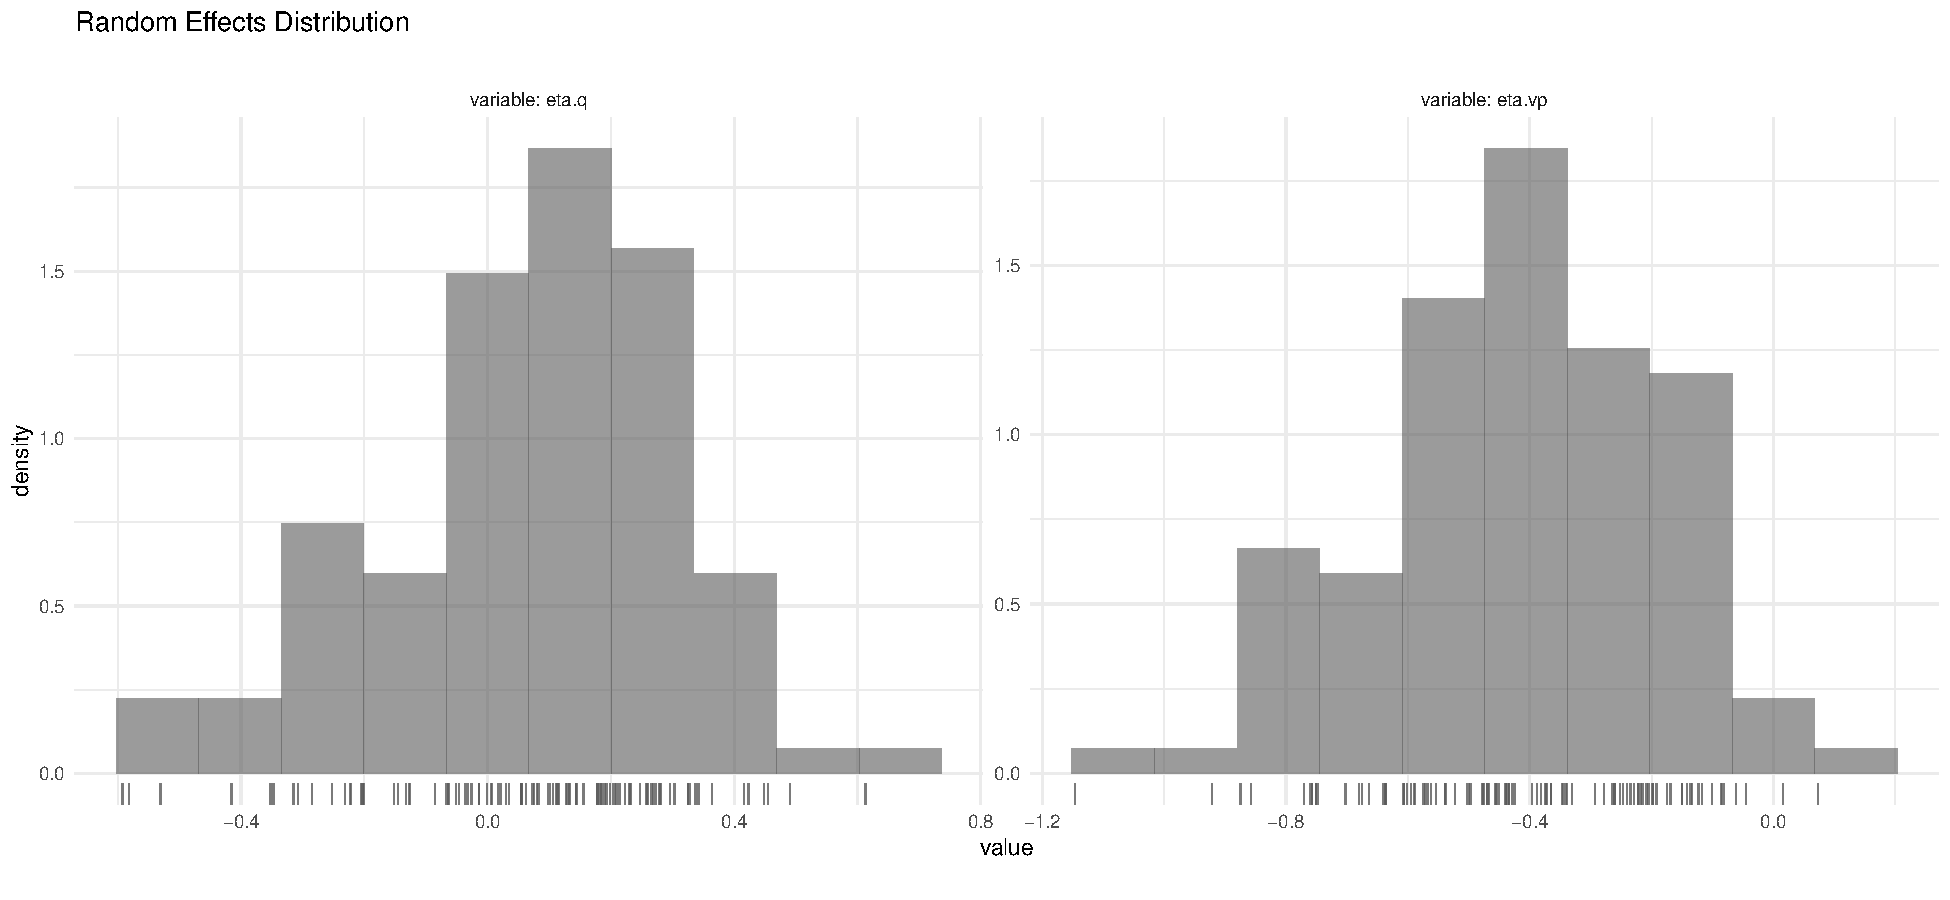
\includegraphics[width=\linewidth]{fig/img/Xpose/eta_distrib.pdf}
        \caption{eta\_distrib}
        \label{fig:eta_distrib}
    \end{subfigure}
    \hfill
    \begin{subfigure}[b]{0.45\linewidth}
        \centering
        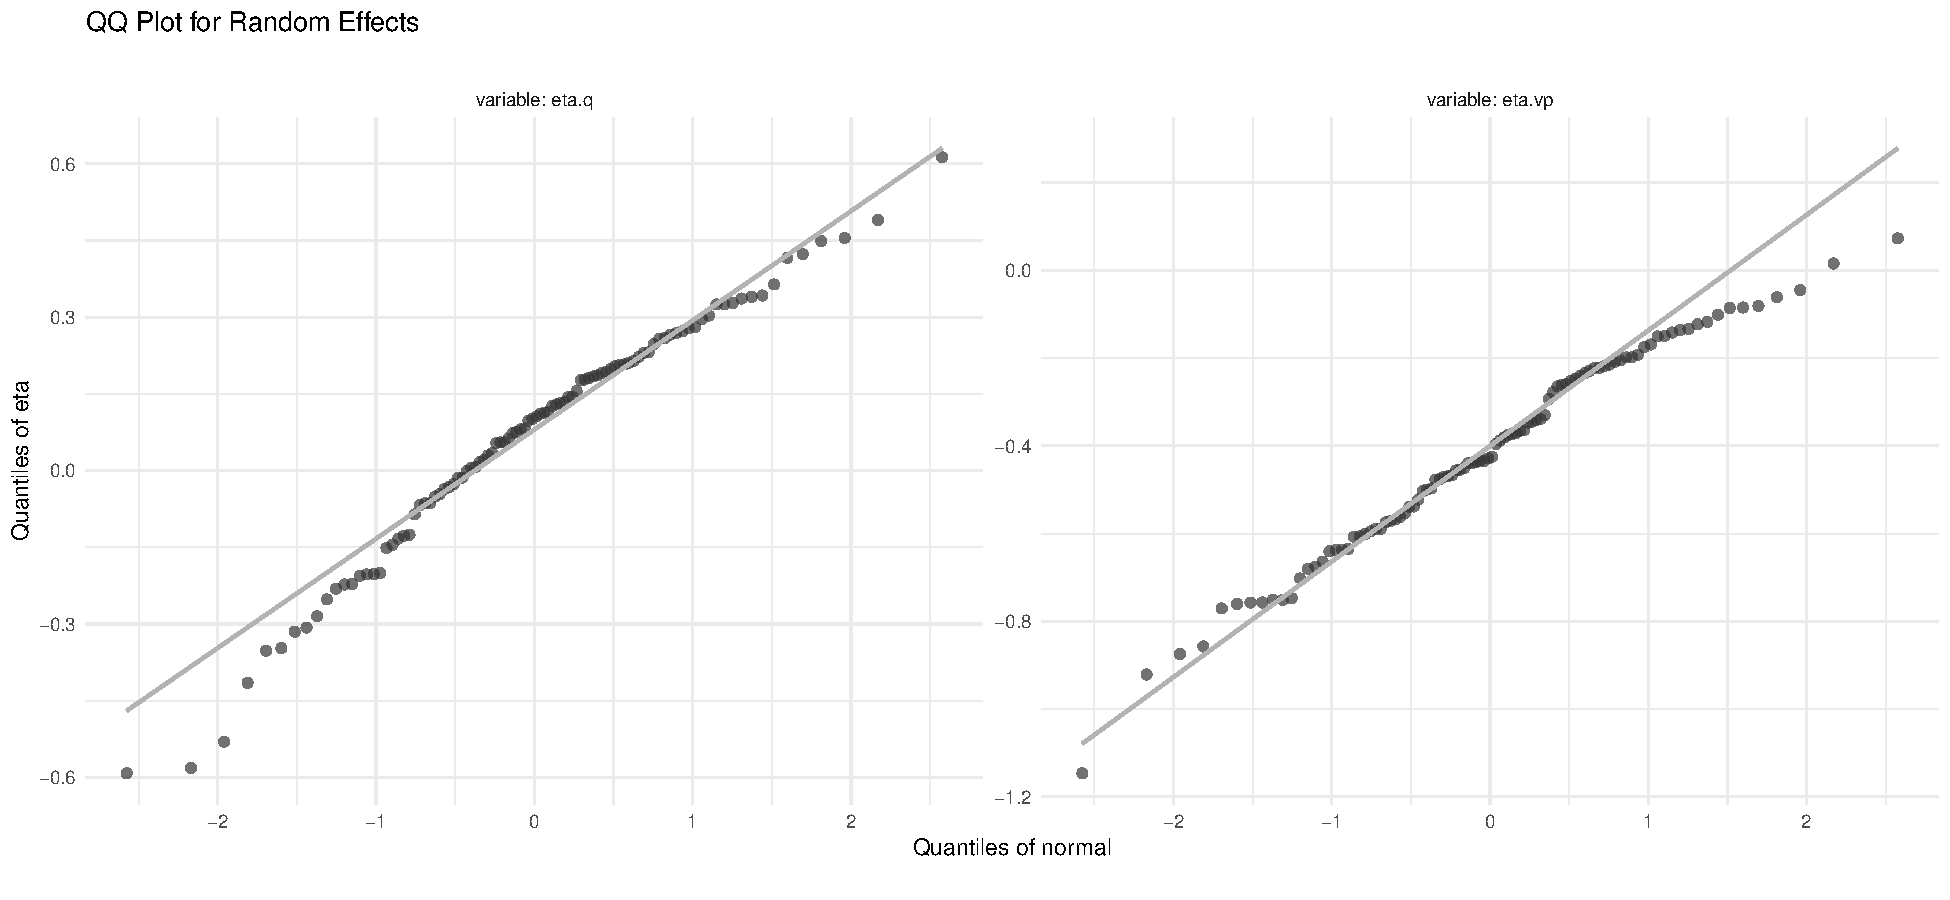
\includegraphics[width=\linewidth]{fig/img/Xpose/eta_qq.pdf}
        \caption{eta\_qq}
        \label{fig:eta_qq}
    \end{subfigure}

    \vspace{1em}

    % Fourth 2x2 grid
    \begin{subfigure}[b]{0.45\linewidth}
        \centering
        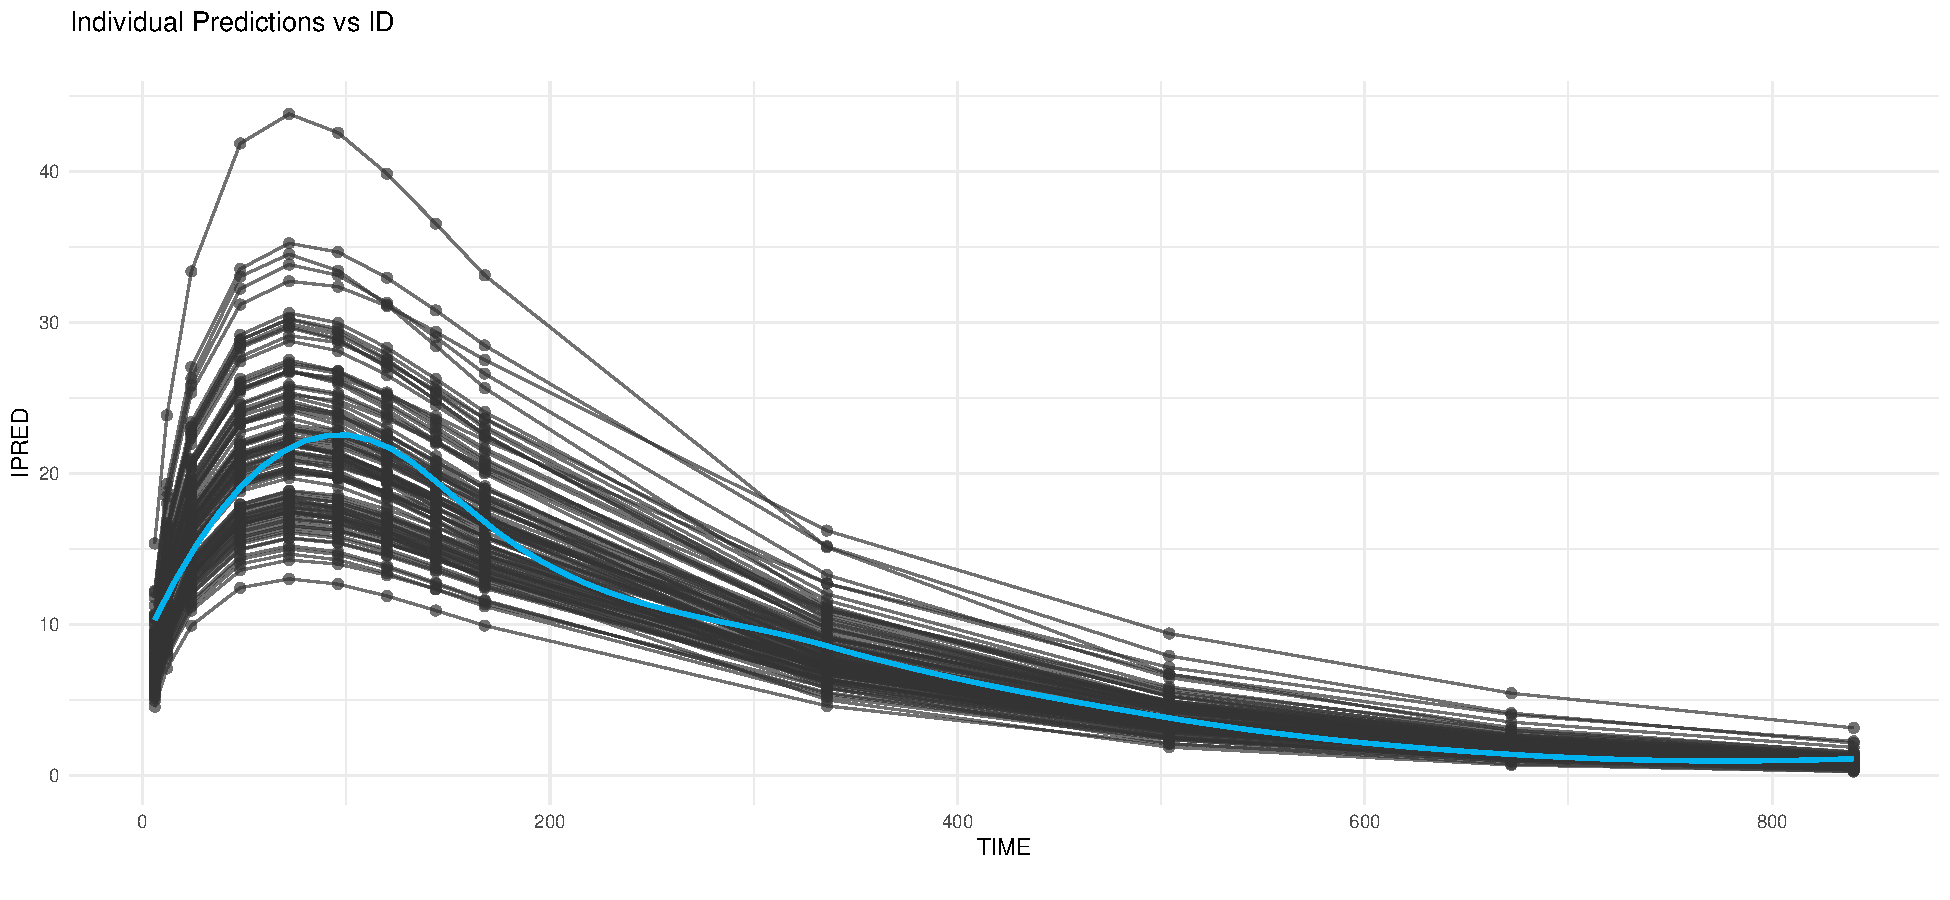
\includegraphics[width=\linewidth]{fig/img/Xpose/ipred_vs_idv.pdf}
        \caption{ipred\_vs\_idv}
        \label{fig:ipred_vs_idv}
    \end{subfigure}
    \hfill
    \begin{subfigure}[b]{0.45\linewidth}
        \centering
        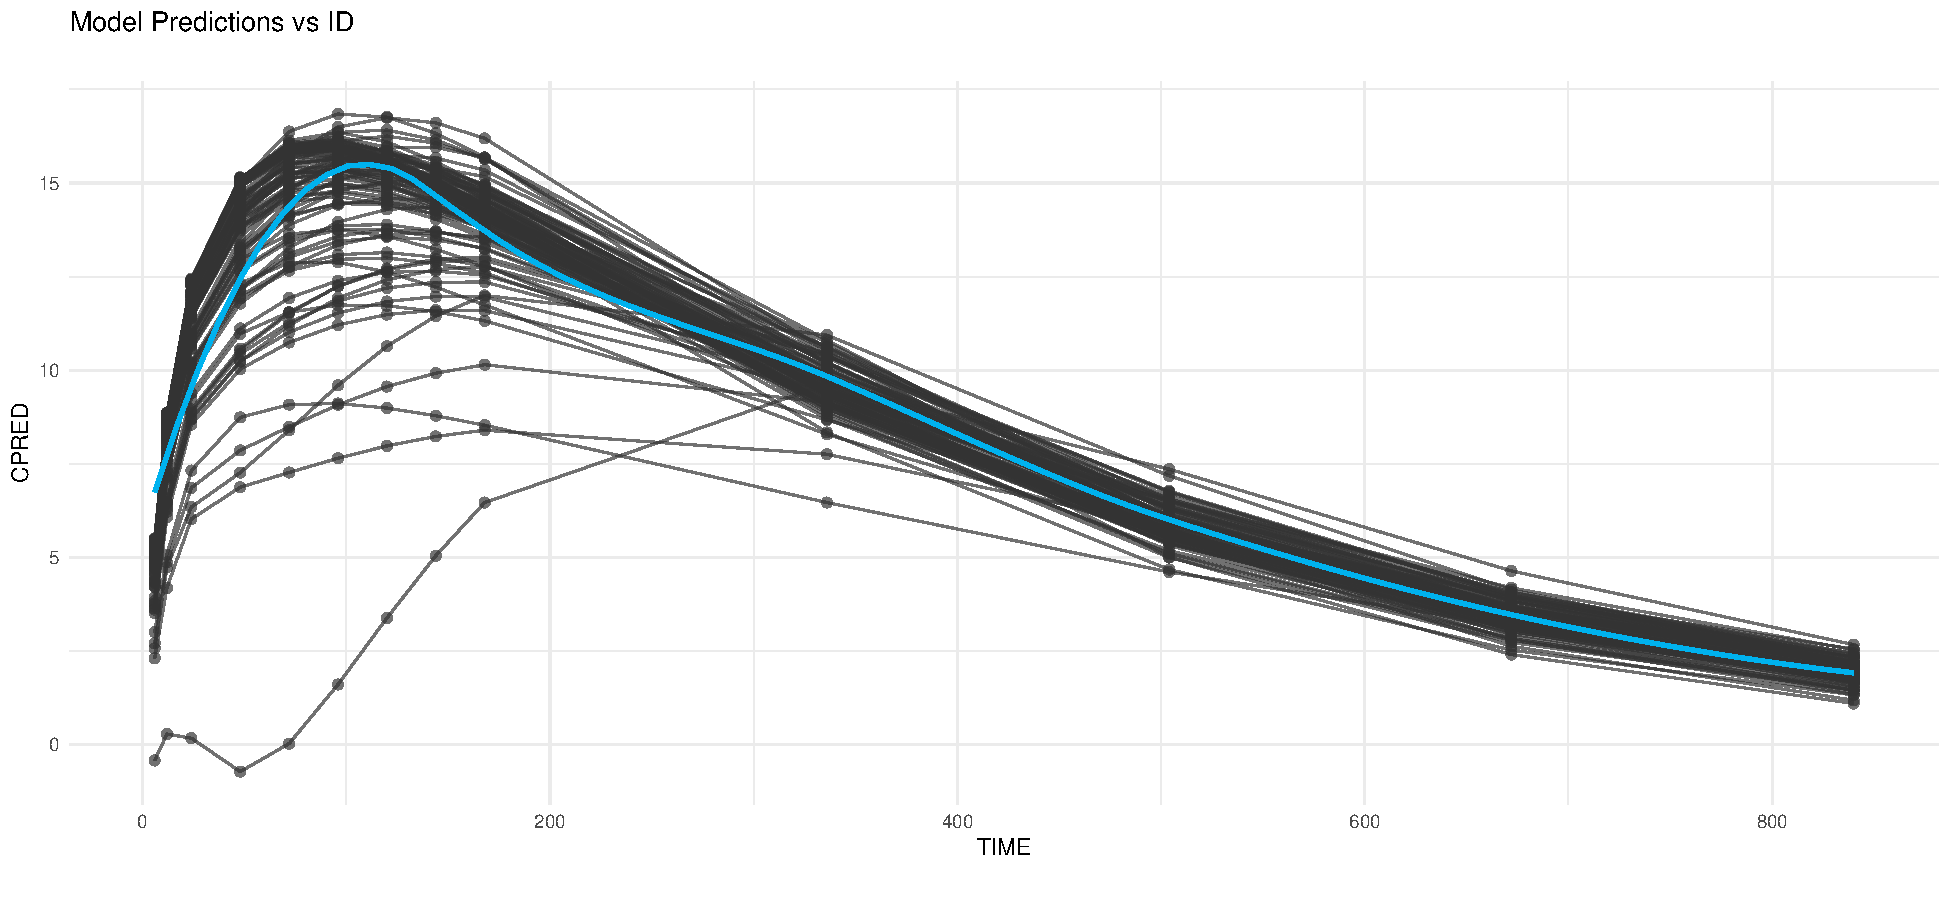
\includegraphics[width=\linewidth]{fig/img/Xpose/pred_vs_idv.pdf}
        \caption{pred\_vs\_idv}
        \label{fig:pred_vs_idv}
    \end{subfigure}

    \vspace{1em}

    % Fifth 2x2 grid
    \begin{subfigure}[b]{0.45\linewidth}
        \centering
        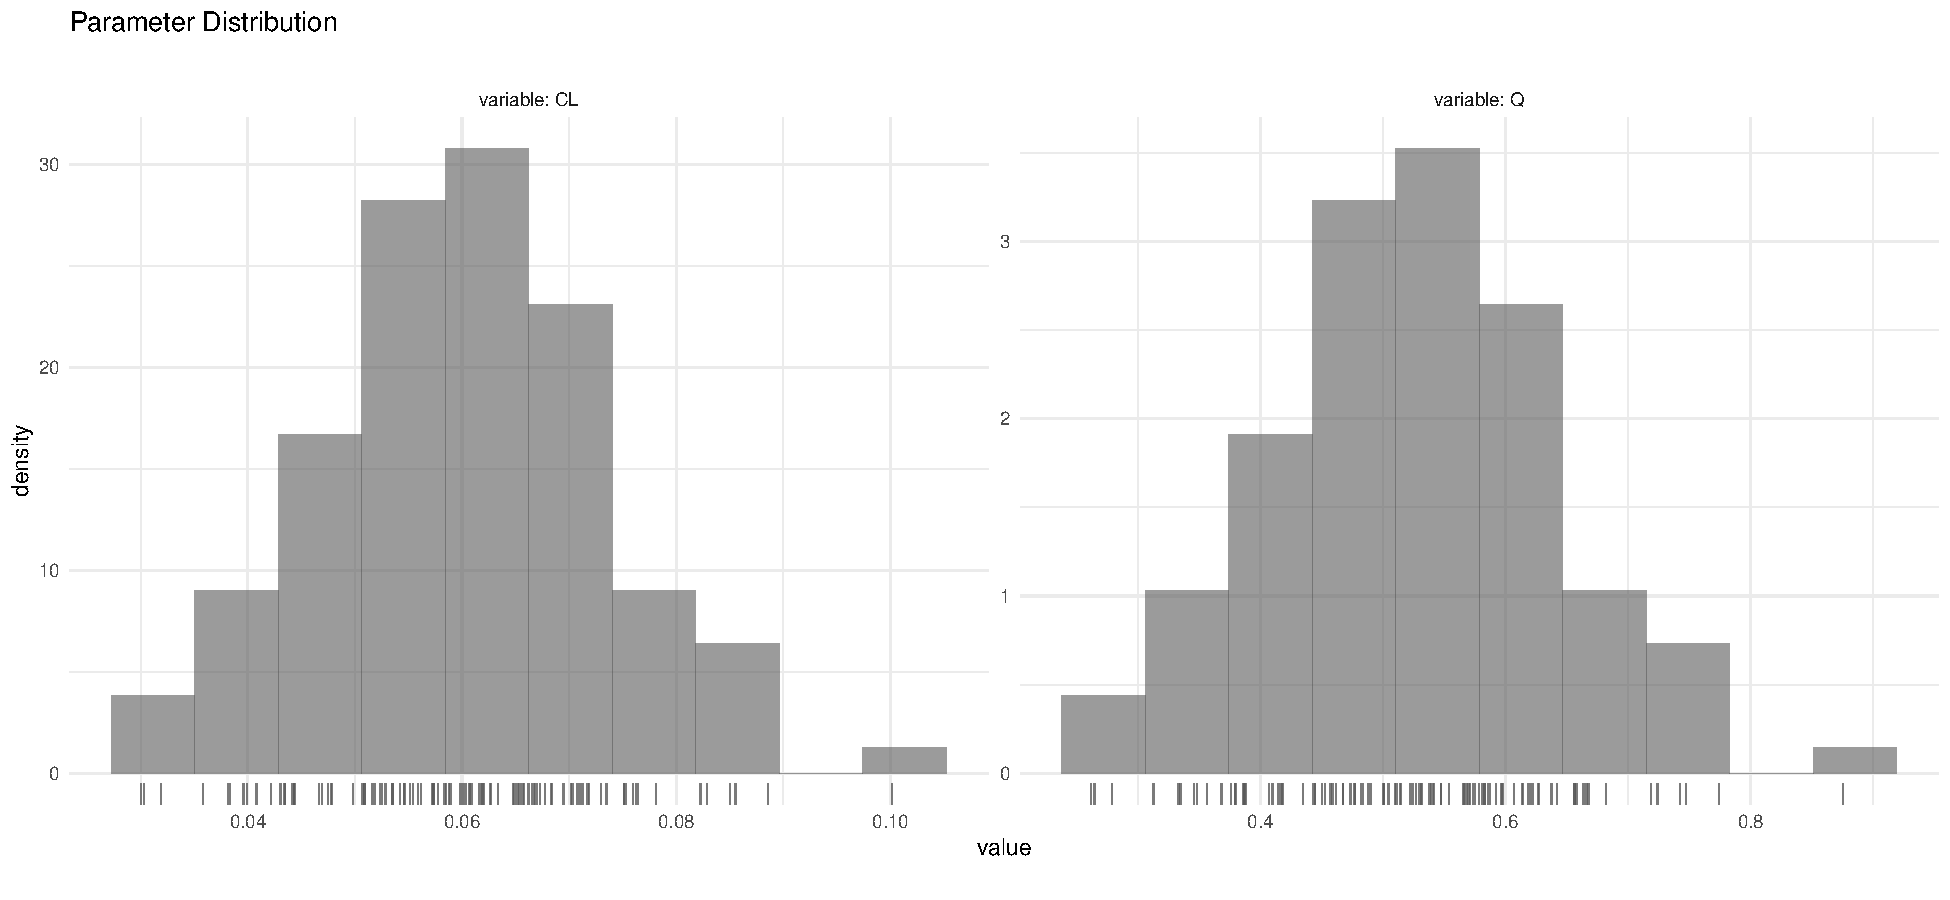
\includegraphics[width=\linewidth]{fig/img/Xpose/prm_distrib.pdf}
        \caption{prm\_distrib}
        \label{fig:prm_distrib}
    \end{subfigure}
    \hfill
    \begin{subfigure}[b]{0.45\linewidth}
        \centering
        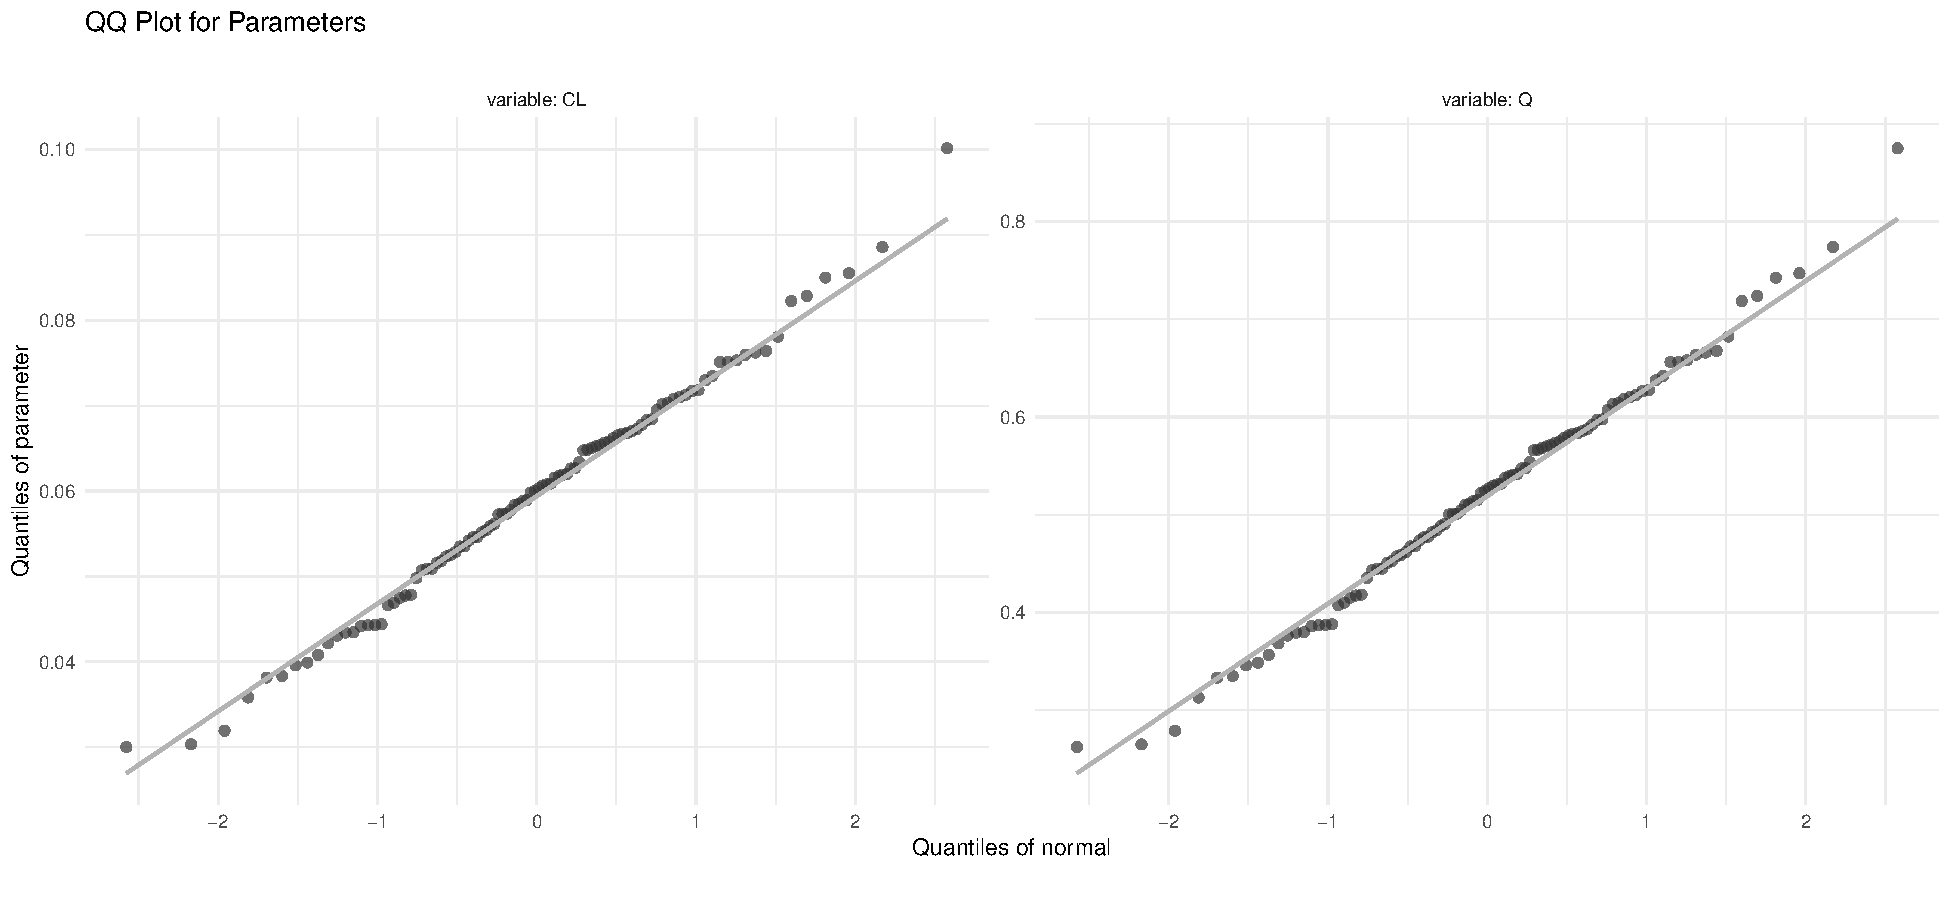
\includegraphics[width=\linewidth]{fig/img/Xpose/prm_qq.pdf}
        \caption{prm\_qq}
        \label{fig:prm_qq}
    \end{subfigure}
\end{figure}




\begin{figure}
\centering
    % Sixth 2x2 grid
    \begin{subfigure}[b]{0.45\linewidth}
        \centering
        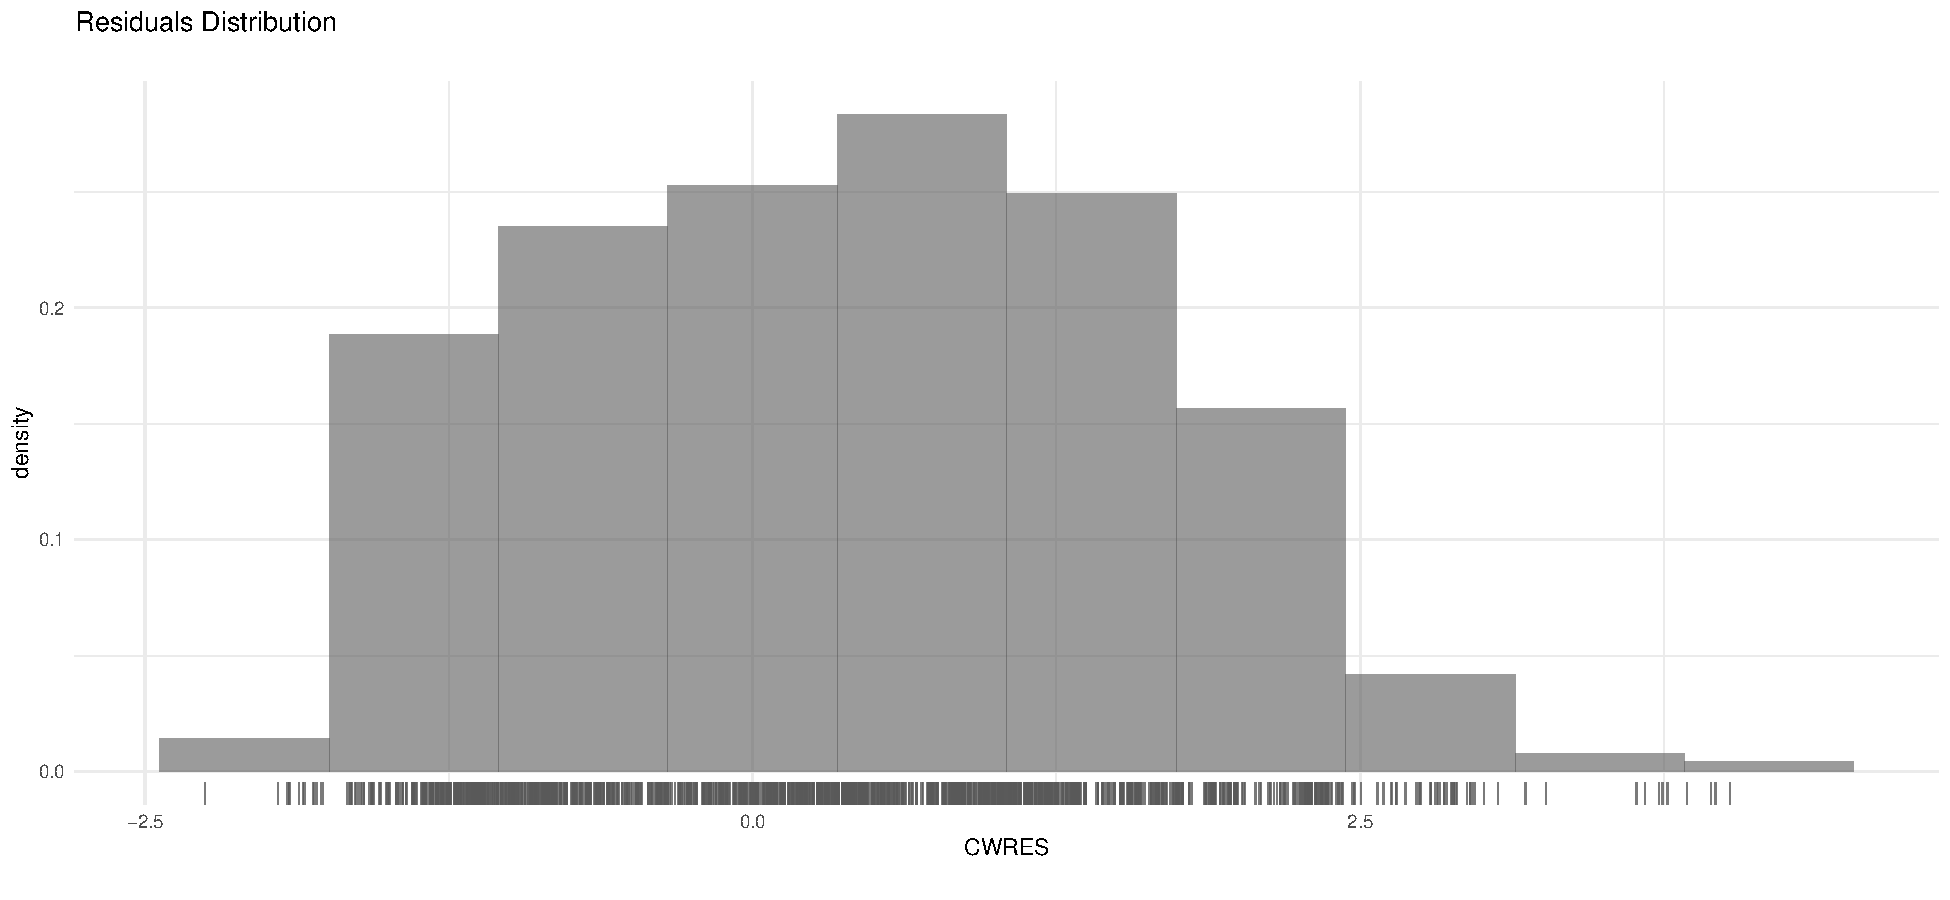
\includegraphics[width=\linewidth]{fig/img/Xpose/res_distrib.pdf}
        \caption{res\_distrib}
        \label{fig:res_distrib}
    \end{subfigure}
    \hfill
    \begin{subfigure}[b]{0.45\linewidth}
        \centering
        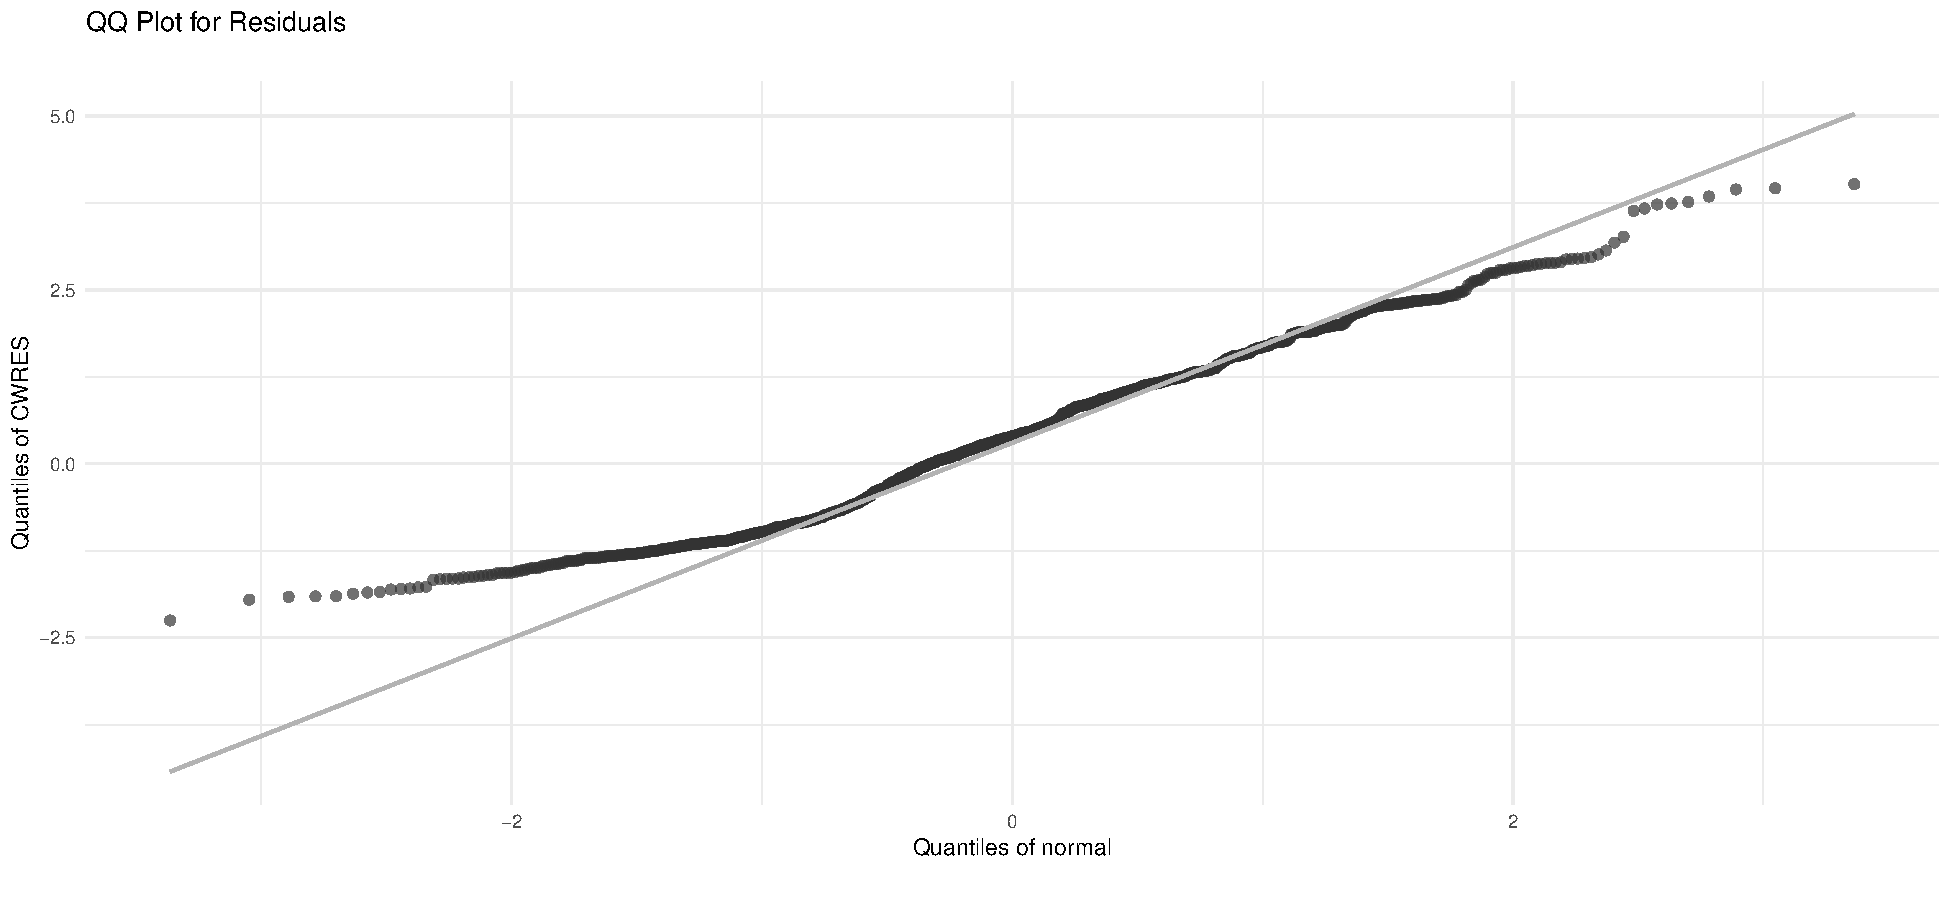
\includegraphics[width=\linewidth]{fig/img/Xpose/res_qq.pdf}
        \caption{res\_qq}
        \label{fig:res_qq}
    \end{subfigure}

    \vspace{1em}

    % Seventh 2x2 grid
    \begin{subfigure}[b]{0.45\linewidth}
        \centering
        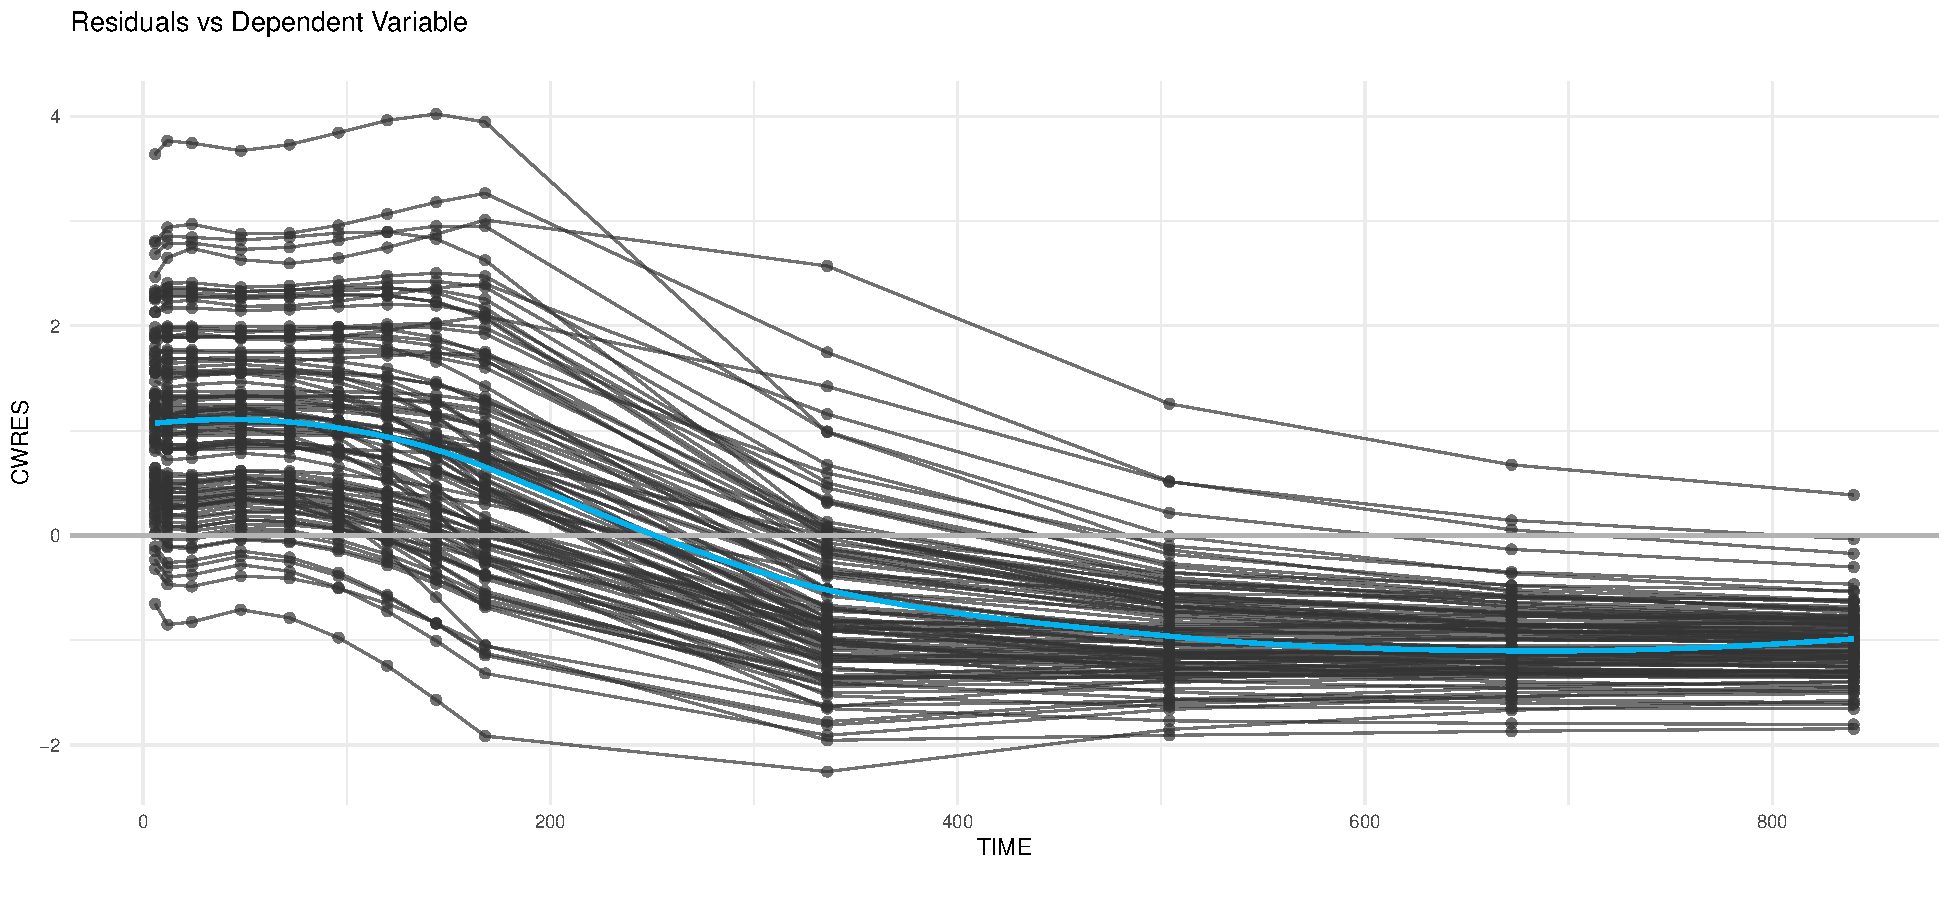
\includegraphics[width=\linewidth]{fig/img/Xpose/res_vs_idv.pdf}
        \caption{res\_vs\_idv}
        \label{fig:res_vs_idv}
    \end{subfigure}
    \hfill
    \begin{subfigure}[b]{0.45\linewidth}
        \centering
        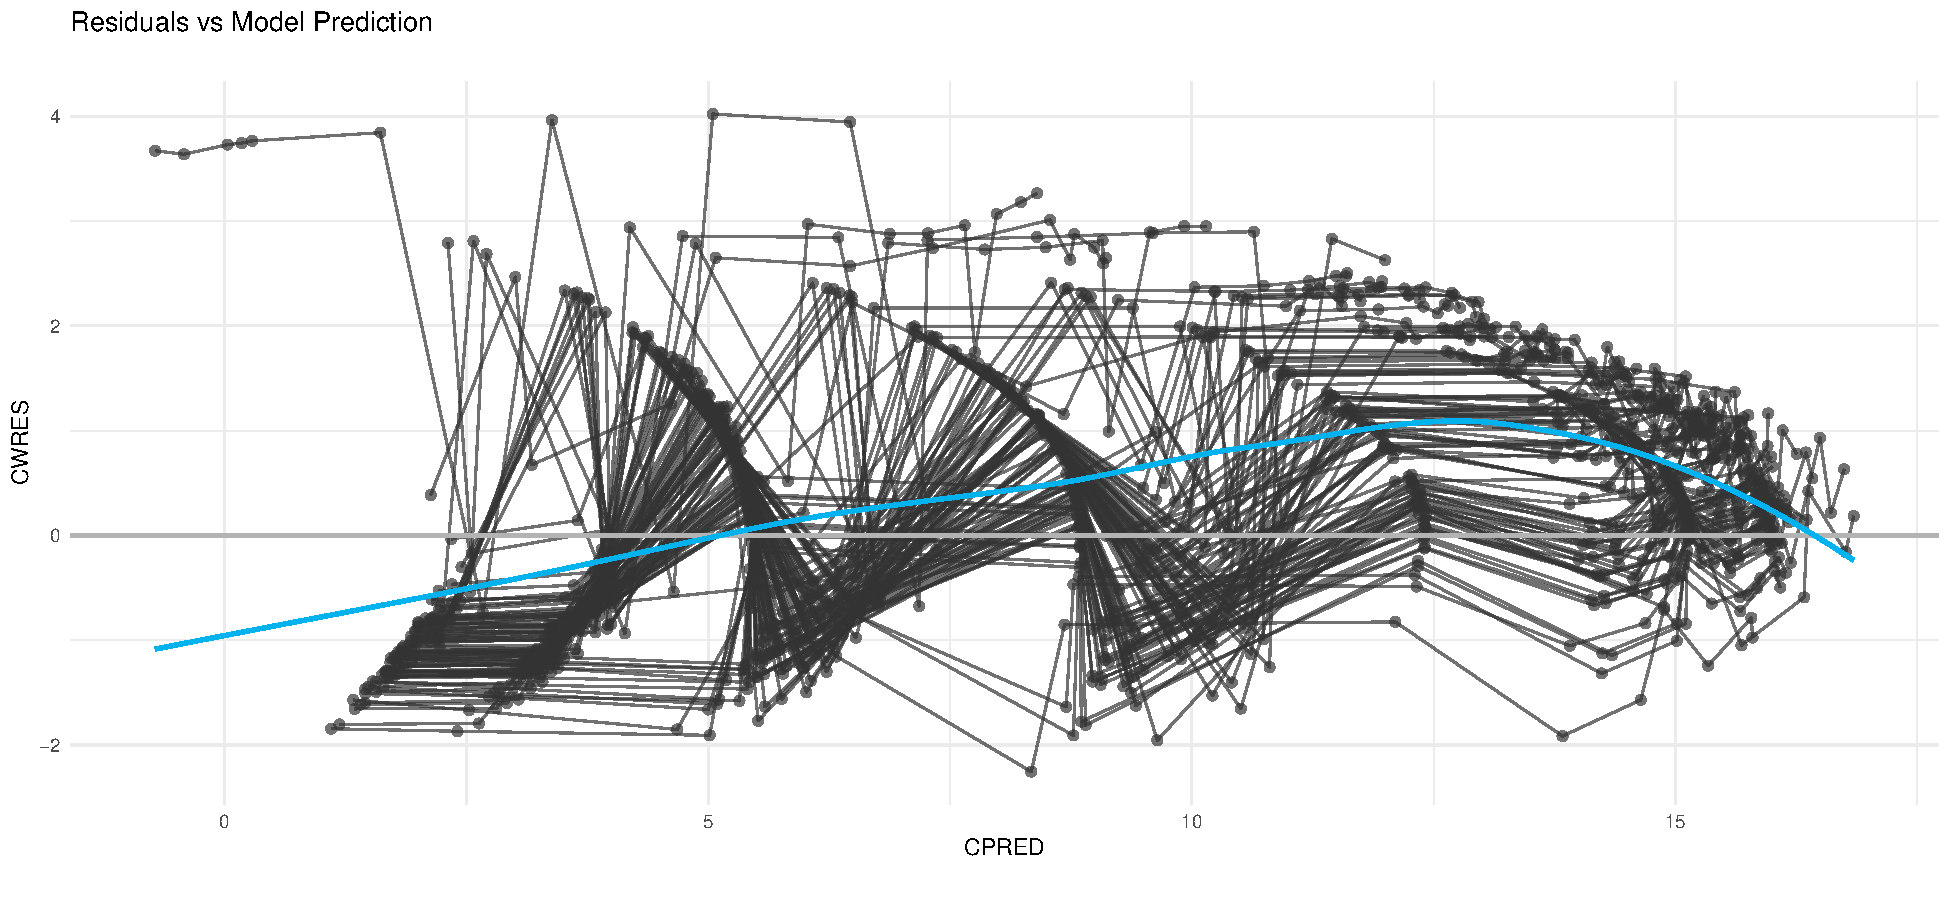
\includegraphics[width=\linewidth]{fig/img/Xpose/res_vs_pred.pdf}
        \caption{res\_vs\_pred}
        \label{fig:res_vs_pred}
    \end{subfigure}

    \caption{Main caption for the figures}
    \label{fig:all_figures}
\end{figure}
% KILDE: Conditional Weighted Residuals (CWRES): A Model Diagnostic - DOI: 10.1007/s11095-007-9361-x
% for the FOCE Method
Firstly, WRES, CWRES, pred, Ipred, dv, and IDV will be explained, as these are used to diagnostic the models. 

The weighted residuals (WRES) are computed as
\begin{align*}
    \text{WRES} = \frac{y_i - \Ex{y_i}_{FO}}{\sqrt{\Cov{y_i}_{FO}}}
\end{align*}

The conditional weighted residuals (CWRES) are computed as
\begin{align*}
    \text{CWRES} = \frac{y_i - \Ex{y_i}_{FOCE}}{\sqrt{\Cov{y_i}_{FOCE}}}
\end{align*}
The FO estimation method assumes the RE is $0$, while the FOCE conditions on the RE. Thus, the RE is accounted for in the CWRES, while the RE is included in the WRES. 

pred refers to the predicted values generated by the model at the population level. These values are computed based on the fixed effects of the model and do not account for individual-specific random effects. They represent the average response for a population based on the covariates included in the model.

Ipred represents the predicted values for individual subjects in a study, incorporating both fixed effects and individual-specific random effects. Ipred values reflect the model's prediction for each subject, taking into account their unique characteristics and the estimated variability.

dv stands for "dependent variable," which typically refers to the observed outcomes or measurement data that the model aims to predict or explain. In pharmacometric analysis, dv is often something like drug concentration measurements over time or other clinical endpoints relevant to the study.

IDV denotes "independent variable" and refers to the variables that are used as predictors in the model. Often, maybe always, the IDV in the plots is considered to be time. IDV variables can help explain the variability in the dv and are essential for building a predictive model.

The blue lines are made by $geom_smooth()$ which is 

The $dv_preds_vs_idv(xpdb_ex_pk)$ function is plotted in Figure \ref{fig:dv_preds_vs_idv}. The function should be read as follows: DV, PRED, IPRED VS. IDV, therefore three plots are created. 















\chapter{nlmixr}

\section{Example 1}

\begin{table}[h]
    \centering
    \begin{tabular}{|l|l|}
        \hline
        \textbf{Variable} & \textbf{Description} \\ 
        \hline
        ID      & Subject ID \\ 
        TIME    & Time (hours) \\ 
        DV      & Drug concentration (mg/L) \\ 
        AMT     & Dose administered (mg) \\ 
        WT      & Weight of the subject (kg) \\ 
        EVID    & Event ID (e.g., dosing event vs. observation) \\ 
        CMT     & Compartment number (for PK models) \\ 
        \hline
    \end{tabular}
    \caption{Description of variables in the \texttt{theo\_sd} dataset.}
    \label{tab:theo_sd}
\end{table}

\section{Marie}
The ini block provides initial values, and is analogous to \$THETA, \$OMEGA and \$SIGMA blocks in NONMEM. The  model block specifies the model, and is analogous to the \$PK, \$PRED and \$ERROR blocks in NONMEM.

Solved PK systems are also currently supported by nlmixr with the ‘linCmt()’ pseudo-function. The solved systems implemented are the one, two and three compartment models with or without first-order absorption. In this example, linCmt() is used, and thus rxode2-based solved PK 1-compartment model with first-order absorption => nlmixr interprets this as a one-compartment model with depot.

The model for $\theta_i = (k_{a,i}, CL_{i}, V_i)^\top$ is
\begin{align*}
    k_{a,i}&=\exp(\beta_1+\eta_{i,k_a}),\\
    CL_i &= \exp(\beta_2+\eta_{i,CL})\\
    V_{i}&=\exp(\beta_3+\eta_{i,V}),\\
\end{align*}
where $\beta_1 = \log(k_a)$, $\beta_2 = \log(CL)$ and $\beta_3=\log(V)$. These are named tka, tcl and tv in lines 6-9. The matrix $\Omega$ is diagonal with elements being the values of eta. The initial values of this are the eta.ka, eta.cl and eta.v values specified in lines 11-13. 

The model $g(\cdot)$ is equivalent with \eqref{eq: conc. one-comp with abs, F=1}.

The residual error is in this example specified to be additive, i.e. $R_i = \sigma^2I$, hence we only need to specify initial values for the sd.

When the model is fitted, the condition values indicate whether the covariance matrix is close to singluar - i.e. if the parameters are strongly correlated.

The Time-lines provide a breakdown of the time taken during various stages of the model fitting process using nlmixr.

The Population Parameters are first of all the estimated values $\hat{\beta}$ and $\hat{\sigma}$ along with their SE. The $\%RSE$ is $RSE(\hat{x})=SE(\hat{x})/\hat{x}$, the relative SE. Back-transformed(95\%CI) are the variables on their original scale (not log-scale) along with CI. BSV is $CV=SD(\hat{x})/\Bar{\hat{x}}*100$. This indicates the relative variability of the parameter estimate among subjects. A higher CV\% suggests greater variability among individuals in terms of the parameter estimated. The shrinkage is a measure of how much the individual estimates (like individual clearance rates) have been pulled towards the population mean (low shrinkage = individual data contributed much).

\section{Mads}

Compartment $1$ only happens at dosing time, so compartment 1 might be the absorption site. We have 12 different individuals with 12 observations each. 

\begin{lstlisting}
    # The PK-model
one.cmt <- function() {
  ini({
    ## You may label each parameter with a comment
    tka <- 0.45 # Log Ka
    tcl <- log(c(0, 2.7, 100)) # Log Cl
    ## This works with interactive models
    ## You may also label the preceding line with label("label text")
    tv <- 3.45; label("log V")
    ## the label("Label name") works with all models
    eta.ka ~ 0.6
    eta.cl ~ 0.3
    eta.v ~ 0.1
    add.sd <- 0.7
  })
  model({
    ka <- exp(tka + eta.ka)
    cl <- exp(tcl + eta.cl)
    v <- exp(tv + eta.v)
    linCmt() ~ add(add.sd)
  })
}

f <- nlmixr(one.cmt)
\end{lstlisting}

Line $4-9$ are the fixed effects. Line $10-13$ are random effects. The sim used for the random effects are used to denote a variance for the random effects. 

Line $14$ is the residual error

Line $17-19$ is $\theta$ i.e. the model parameters. Note that they include a random effect and a fixed effect

Line $20$ is the residual variance model chosen. 

In this model no ODEs are specified. If this was included, it should have been a part of the model({})


For the fixed effects:
\begin{itemize}
    \item tka is the log absorption rate
    \item tcl is the elimination rate.
    \item tv is the log volume of distribution
\end{itemize}
tcl is a vector with $3$ entries. You can do that with all fixed effects, and in this case it means that the effect can vary from 0-100, but it should start at 2.7.

Remember eta is the greek letter.

In model({}) the parameters are specified as:
\begin{align*}
    K_{a}&=\exp(log(0.45)+\eta),  \quad \eta \sim 0.6\\
     Cl &= \exp(log(2.7) + \eta), \quad \eta \sim 0.3\\
    V_{d}&=\exp(log(3.45) + \eta), \quad \eta \sim 0.1\\
\end{align*}

When fitting the model, the nlmixr() function is used. 
\begin{lstlisting}
    nlmixr(
model,
data,
est = "saem",
saemControl(print=50,
nBurn=200, nEm=300),
tableControl(cwres=TRUE))
\end{lstlisting}
The first three inputs are self explanatory. 

Saemcontrol() takes the inputs: 
\begin{itemize}
  \item \texttt{seed} \hfill Random seed: (99)
  \item \texttt{nBurn} \hfill Number of iterations in the SA (burn-in) step: (200)
  \item \texttt{nEm} \hfill Number of iterations in the EM step: (300)
  \item \texttt{nmc} \hfill Number of Markov chains: (3)
  \item \texttt{atol} \hfill Absolute convergence tolerance: (1e-8)
  \item \texttt{print} \hfill Iterations to complete before printing to console: (1)
  \item \texttt{...} \hfill Additional arguments
\end{itemize}
i.e. its the specifications for the estimation method. If the estimation methods $est = "focei", "foce", "foi", "fo"$ were used, then $foceiControl()$ could have been used. 

The tablecontrol takes the inputs: 
\begin{itemize}
  \item \texttt{cwres} \hfill Boolean indicating if you need to calculate conditional weighted residuals (CWRES). This is on by default for FOCE(i) routines. This will also generate WRES, CPRED, and CRES.
  \item \texttt{npde} \hfill Calculate npde residuals (NPDE). This will also generate EPRED and ERES.
  \item \texttt{nsim} \hfill Number of simulations used for NPDE: (default 300)
  \item \texttt{ties} \hfill Boolean indicating if noise will be added to avoid ties in NPDE calculation: (TRUE)
  \item \texttt{Seed} \hfill Random seed to use for NPDE calculation: (1009)
\end{itemize}


\begin{lstlisting}
fit <- nlmixr(one.cmt, theo_sd, est="saem",
              control=list(print=0))

print(fit)
\end{lstlisting}

Breakdown of the print: 

First is the time:
\begin{lstlisting}
     Time (sec fit$time):

        covariance  saem table compress other
elapsed       0.01 41.27  0.04     0.02  3.61
\end{lstlisting}
This gives the time it took the program during the fitting process. 

Next are the population parameter
\begin{lstlisting}
    Population Parameters (fit$parFixed or fit$parFixedDf):

       Parameter  Est.     SE %RSE Back-transformed(95%CI) BSV(CV%) Shrink(SD)%
tka       Log Ka 0.453  0.195 43.1       1.57 (1.07, 2.31)     71.4    -0.445%
tcl       Log Cl  1.02 0.0843 8.29       2.76 (2.34, 3.26)     27.2      3.88%
tv         log V  3.45 0.0467 1.35       31.5 (28.8, 34.5)     13.9      10.2%
add.sd           0.695                               0.695
\end{lstlisting}
"Parameter" is the parameter being estimated. Est. is the estimated value. SE is the standard error. \%RSE is the relative standard error. Back-transformed is the transformation back to the original scale and the 95\% confidence interval. BSV is the between subject variability. Shrink ??



\chapter{Data}
\section{Introduction}
The PK models in this section will be fitted using NLMM with the nlmixr2 package \citep{nlmixr, nlmixrarticle}. To be able to fit a model, a model specification, a dataset, and an estimation method must be provided.

The model specification must include initial values and potential boundaries for $\beta$, residual error variance, $\sigma^2$, and for the entries in $\Omega$. The functional forms of the $p$ entries in $d$ from \eqref{eq: NLME Stage 2}, along with the error model, must be specified.
The functional form of \ref{eq: NLME Stage 1} is specified by solving a system of given ODEs describing the mass balance equations for the given compartments, e.g. \eqref{eq: first order kinetic of amount in one com without abs}, \eqref{eq: first order kinetic of amount in central com with abs com}, or \eqref{eq: 2-comp central}.

% data structure
The data require at least a unique subject identifier, timestamp of the observations, a dependent variable, an amount or rate of drug, and an event identifier to describe the observation \citep{nlmixrarticle}. 

% estimation method
The FOCEI, covered in \ref{sec: Estimation methods}, is used as the estimation method, however, other methods, e.g. FO, FOCE, and saem, are also supported. 


%output
% The output of the nlmixr function is metrics of goodness of fit, i.e. objective function, information criteria, log likelihood, and condition number, the run time of the fitting process, the subject specific parameters with standard errors, residual squared error, BSV, and shrinkage, the fitted omega matrix and lastly the fitted data 

% metrics of goodness of fit
% The run time to fit the model
% the population parameter estimates + residual error
% Omega matrix
% fitted values for $\beta$s, $\eta$s and $\e_i$s
\section{Introduction to data}
\section{Questions}
\begin{itemize}
    \item What is the point of fitting models on cp?
    \item Number of models - number of subjects, CP/DV
    \item Initial values
    \item Covariate model
    \item How much in depth good of fitness should we do for the models
    \item Should we expect more/new data or models?
\end{itemize}


\section{Model without iiv}
\subsection{10 sample profile}
\begin{table}
\centering\centering
\caption{No BSV - CP 10}
\centering
\fontsize{8}{10}\selectfont
\begin{tabular}[t]{lllllll}
\toprule
\textbf{Parameter} & \textbf{Est} & \textbf{SE} & \textbf{\%RSE} & \textbf{Back-transformed} & \textbf{BSV} & \textbf{Shrinkage}\\
\midrule
tka & -5.39 & 0.806 & 15 & 0.00456 (0.00094, 0.0222) &  & \\
\midrule
tq & -3.05 & 1.3 & 42.6 & 0.0473 (0.00371, 0.603) &  & \\
\midrule
tcl & -2.94 & 0.0613 & 2.09 & 0.0529 (0.0469, 0.0597) &  & \\
\midrule
tvc & -0.104 & 0.965 & 923 & 0.901 (0.136, 5.97) &  & \\
\midrule
tvp & 1.51 & 1.85 & 123 & 4.51 (0.119, 171) &  & \\
\midrule
prop.sd & 0.429 &  &  & 0.429 &  & \\
\bottomrule
\end{tabular}
\end{table}

\begin{table}
\centering\centering
\caption{No BSV - DV 10}
\centering
\fontsize{8}{10}\selectfont
\begin{tabular}[t]{lllllll}
\toprule
\textbf{Parameter} & \textbf{Est} & \textbf{SE} & \textbf{\%RSE} & \textbf{Back-transformed} & \textbf{BSV} & \textbf{Shrinkage}\\
\midrule
tka & -4.48 & 0.648 & 14.5 & 0.0113 (0.00318, 0.0403) &  & \\
\midrule
tq & -1.51 & 0.994 & 65.9 & 0.221 (0.0315, 1.55) &  & \\
\midrule
tcl & -2.96 & 0.0561 & 1.9 & 0.0521 (0.0466, 0.0581) &  & \\
\midrule
tvc & 0.697 & 0.664 & 95.2 & 2.01 (0.547, 7.37) &  & \\
\midrule
tvp & 2.35 & 0.243 & 10.4 & 10.4 (6.48, 16.8) &  & \\
\midrule
prop.sd & 0.428 &  &  & 0.428 &  & \\
\bottomrule
\end{tabular}
\end{table}

\begin{itemize}
    \item DV vs. CP: Lavere sd for CP. 
    \item Betydeligt højere estimeret F, VC, og desuden generelt højere estimerede værdier for CP
    \item SE generelt lavere for DV
\end{itemize}

\subsection{25 sample profile}
\begin{table}
\centering\centering
\caption{No BSV - CP 25}
\centering
\fontsize{8}{10}\selectfont
\begin{tabular}[t]{lllllll}
\toprule
\textbf{Parameter} & \textbf{Est} & \textbf{SE} & \textbf{\%RSE} & \textbf{Back-transformed} & \textbf{BSV} & \textbf{Shrinkage}\\
\midrule
tka & -4.08 & 0.812 & 19.9 & 0.0169 (0.00344, 0.083) &  & \\
\midrule
tq & -0.874 & 1.19 & 136 & 0.417 (0.0404, 4.31) &  & \\
\midrule
tcl & -2.9 & 0.0369 & 1.27 & 0.0553 (0.0514, 0.0594) &  & \\
\midrule
tvc & 1.12 & 0.681 & 60.7 & 3.07 (0.808, 11.7) &  & \\
\midrule
tvp & 2.6 & 0.139 & 5.34 & 13.4 (10.2, 17.7) &  & \\
\midrule
prop.sd & 0.487 &  &  & 0.487 &  & \\
\bottomrule
\end{tabular}
\end{table}
\begin{itemize}
    \item DV10 vs. DV25: Higher sd for 25sp
\end{itemize}

\begin{table}
\centering\centering
\caption{No BSV - DV 25}
\centering
\fontsize{8}{10}\selectfont
\begin{tabular}[t]{lllllll}
\toprule
\textbf{Parameter} & \textbf{Est} & \textbf{SE} & \textbf{\%RSE} & \textbf{Back-transformed} & \textbf{BSV} & \textbf{Shrinkage}\\
\midrule
tka & -3.81 & 0.787 & 20.7 & 0.0222 (0.00475, 0.104) &  & \\
\midrule
tq & -0.444 & 1.25 & 282 & 0.641 (0.0551, 7.47) &  & \\
\midrule
tcl & -2.88 & 0.0378 & 1.31 & 0.0562 (0.0522, 0.0605) &  & \\
\midrule
tvc & 1.29 & 0.621 & 48 & 3.65 (1.08, 12.3) &  & \\
\midrule
tvp & 2.69 & 0.129 & 4.78 & 14.7 (11.4, 18.9) &  & \\
\midrule
prop.sd & 0.508 &  &  & 0.508 &  & \\
\bottomrule
\end{tabular}
\end{table}


\subsection{50 sample profile}
\begin{table}
\centering\centering
\caption{No BSV - CP 50}
\centering
\fontsize{8}{10}\selectfont
\begin{tabular}[t]{lllllll}
\toprule
\textbf{Parameter} & \textbf{Est} & \textbf{SE} & \textbf{\%RSE} & \textbf{Back-transformed} & \textbf{BSV} & \textbf{Shrinkage}\\
\midrule
tka & -5.88 & 0.0419 & 0.713 & 0.0028 (0.00258, 0.00304) &  & \\
\midrule
tq & -4.81 & 1.17 & 24.3 & 0.00815 (0.000821, 0.0809) &  & \\
\midrule
tcl & -3.02 & 0.198 & 6.55 & 0.0488 (0.0331, 0.0719) &  & \\
\midrule
tvc & -0.352 & 0.0959 & 27.2 & 0.703 (0.583, 0.849) &  & \\
\midrule
tvp & 5.48 & 4.22 & 76.9 & 241 (0.0619, 9.35e+05) &  & \\
\midrule
prop.sd & 0.485 &  &  & 0.485 &  & \\
\bottomrule
\end{tabular}
\end{table}

\begin{table}
\centering\centering
\caption{No BSV - DV 50}
\centering
\fontsize{8}{10}\selectfont
\begin{tabular}[t]{lllllll}
\toprule
\textbf{Parameter} & \textbf{Est} & \textbf{SE} & \textbf{\%RSE} & \textbf{Back-transformed} & \textbf{BSV} & \textbf{Shrinkage}\\
\midrule
tka & -5.91 & 0.0658 & 1.11 & 0.00272 (0.00239, 0.0031) &  & \\
\midrule
tq & -4.36 & 2.18 & 50 & 0.0127 (0.000177, 0.916) &  & \\
\midrule
tcl & -3.09 & 0.596 & 19.3 & 0.0456 (0.0142, 0.147) &  & \\
\midrule
tvc & -0.369 & 0.115 & 31.1 & 0.691 (0.552, 0.866) &  & \\
\midrule
tvp & 4.62 & 4.22 & 91.3 & 102 (0.0261, 3.95e+05) &  & \\
\midrule
prop.sd & 0.51 &  &  & 0.51 &  & \\
\bottomrule
\end{tabular}
\end{table}


\subsection{100 sample profile}
\begin{table}
\centering\centering
\caption{No BSV - CP 100}
\centering
\fontsize{8}{10}\selectfont
\begin{tabular}[t]{lllllll}
\toprule
\textbf{Parameter} & \textbf{Est} & \textbf{SE} & \textbf{\%RSE} & \textbf{Back-transformed} & \textbf{BSV} & \textbf{Shrinkage}\\
\midrule
tka & -3.36 & 0.305 & 9.07 & 0.0347 (0.0191, 0.063) &  & \\
\midrule
tq & 0.234 & 0.631 & 270 & 1.26 (0.367, 4.35) &  & \\
\midrule
tcl & -2.9 & 0.0187 & 0.644 & 0.0548 (0.0528, 0.0568) &  & \\
\midrule
tvc & 1.61 & 0.362 & 22.5 & 5.01 (2.46, 10.2) &  & \\
\midrule
tvp & 2.67 & 0.12 & 4.5 & 14.4 (11.4, 18.2) &  & \\
\midrule
prop.sd & 0.486 &  &  & 0.486 &  & \\
\bottomrule
\end{tabular}
\end{table}

\begin{table}
\centering\centering
\caption{No BSV - DV 100}
\centering
\fontsize{8}{10}\selectfont
\begin{tabular}[t]{lllllll}
\toprule
\textbf{Parameter} & \textbf{Est} & \textbf{SE} & \textbf{\%RSE} & \textbf{Back-transformed} & \textbf{BSV} & \textbf{Shrinkage}\\
\midrule
tka & -5.92 & 0.0529 & 0.893 & 0.00267 (0.00241, 0.00296) &  & \\
\midrule
tq & -3.69 & 0.248 & 6.71 & 0.0249 (0.0153, 0.0405) &  & \\
\midrule
tcl & -3.49 & 0.203 & 5.83 & 0.0305 (0.0204, 0.0454) &  & \\
\midrule
tvc & -0.423 & 0.0844 & 20 & 0.655 (0.555, 0.773) &  & \\
\midrule
tvp & 6.02 & 1.47 & 24.4 & 412 (23.1, 7.35e+03) &  & \\
\midrule
prop.sd & 0.49 &  &  & 0.49 &  & \\
\bottomrule
\end{tabular}
\end{table}

\section{Model with ETAs on CL and Q}
\subsection{10 sample profile}
\begin{table}
\centering\centering
\caption{ETA CLQ CP 10}
\centering
\fontsize{8}{10}\selectfont
\begin{tabular}[t]{lllllll}
\toprule
\textbf{Parameter} & \textbf{Est} & \textbf{SE} & \textbf{\%RSE} & \textbf{Back-transformed} & \textbf{BSV} & \textbf{Shrinkage}\\
\midrule
tka & -3.66 & 2.8 & 76.6 & 0.0258 (0.000107, 6.26) &  & \\
\midrule
tq & -1.2 & 14.2 & 1.19e+03 & 0.302 (2.45e-13, 3.73e+11) &  & \\
\midrule
tcl & -3.41 & 0.186 & 5.46 & 0.0331 (0.023, 0.0477) &  & \\
\midrule
tvc & 1.18 & 3.28 & 278 & 3.25 (0.00522, 2.03e+03) &  & \\
\midrule
tvp & 1.32 & 3.14 & 238 & 3.74 (0.00787, 1.78e+03) &  & \\
\midrule
prop.sd & 0.117 &  &  & 0.117 &  & \\
\midrule\\
eta.q &  &  &  &  & 9.33 & -3.17\%>\\
\bottomrule
\end{tabular}
\end{table}
\begin{table}
\centering\centering
\caption{ETA CLQ DV 10}
\centering
\fontsize{8}{10}\selectfont
\begin{tabular}[t]{lllllll}
\toprule
\textbf{Parameter} & \textbf{Est} & \textbf{SE} & \textbf{\%RSE} & \textbf{Back-transformed} & \textbf{BSV} & \textbf{Shrinkage}\\
\midrule
tka & -3.56 & 0.0155 & 0.435 & 0.0284 (0.0275, 0.0292) &  & \\
\midrule
tq & -0.93 & 0.115 & 12.4 & 0.394 (0.315, 0.495) &  & \\
\midrule
tcl & -3.41 & 0.0434 & 1.27 & 0.0332 (0.0305, 0.0361) &  & \\
\midrule
tvc & 1.23 & 0.0909 & 7.37 & 3.44 (2.87, 4.11) &  & \\
\midrule
tvp & 1.31 & 0.0164 & 1.25 & 3.72 (3.6, 3.84) &  & \\
\midrule
prop.sd & 0.155 &  &  & 0.155 &  & \\
\midrule\\
eta.q &  &  &  &  & 9.15 & -0.392\%>\\
\bottomrule
\end{tabular}
\end{table}
\subsection{25 sample profile}
\begin{table}
\centering\centering
\caption{ETA CLQ CP 25}
\centering
\fontsize{8}{10}\selectfont
\begin{tabular}[t]{lllllll}
\toprule
\textbf{Parameter} & \textbf{Est} & \textbf{SE} & \textbf{\%RSE} & \textbf{Back-transformed} & \textbf{BSV} & \textbf{Shrinkage}\\
\midrule
tka & -3.76 & 0.819 & 21.8 & 0.0233 (0.00468, 0.116) &  & \\
\midrule
tq & -1.41 & 2.73 & 193 & 0.243 (0.00115, 51.2) &  & \\
\midrule
tcl & -3.39 & 0.117 & 3.46 & 0.0336 (0.0267, 0.0423) &  & \\
\midrule
tvc & 1.11 & 0.691 & 62.5 & 3.02 (0.78, 11.7) &  & \\
\midrule
tvp & 1.37 & 0.632 & 46.1 & 3.94 (1.14, 13.6) &  & \\
\midrule
prop.sd & 0.152 &  &  & 0.152 &  & \\
\midrule\\
eta.q &  &  &  &  & 13.5 & 0.372\%<\\
\bottomrule
\end{tabular}
\end{table}
\begin{table}
\centering\centering
\caption{ETA CLQ DV 25}
\centering
\fontsize{8}{10}\selectfont
\begin{tabular}[t]{lllllll}
\toprule
\textbf{Parameter} & \textbf{Est} & \textbf{SE} & \textbf{\%RSE} & \textbf{Back-transformed} & \textbf{BSV} & \textbf{Shrinkage}\\
\midrule
tka & -3.62 & 0.519 & 14.3 & 0.0267 (0.00965, 0.0737) &  & \\
\midrule
tq & -1 & 1.5 & 149 & 0.366 (0.0193, 6.95) &  & \\
\midrule
tcl & -3.39 & 0.0485 & 1.43 & 0.0338 (0.0308, 0.0372) &  & \\
\midrule
tvc & 1.11 & 0.126 & 11.4 & 3.03 (2.36, 3.87) &  & \\
\midrule
tvp & 1.42 & 0.0319 & 2.25 & 4.15 (3.89, 4.41) &  & \\
\midrule
prop.sd & 0.183 &  &  & 0.183 &  & \\
\midrule\\
eta.q &  &  &  &  & 15.8 & 13.0\%<\\
\bottomrule
\end{tabular}
\end{table}
\subsection{50 sample profile}
\begin{table}
\centering\centering
\caption{ETA CLQ CP 50}
\centering
\fontsize{8}{10}\selectfont
\begin{tabular}[t]{lllllll}
\toprule
\textbf{Parameter} & \textbf{Est} & \textbf{SE} & \textbf{\%RSE} & \textbf{Back-transformed} & \textbf{BSV} & \textbf{Shrinkage}\\
\midrule
tka & -3.81 & 0.288 & 7.56 & 0.0223 (0.0127, 0.0391) &  & \\
\midrule
tq & -1.36 & 0.654 & 48.1 & 0.257 (0.0712, 0.924) &  & \\
\midrule
tcl & -3.34 & 0.0651 & 1.95 & 0.0354 (0.0311, 0.0402) &  & \\
\midrule
tvc & 1.08 & 0.261 & 24.3 & 2.94 (1.76, 4.9) &  & \\
\midrule
tvp & 1.49 & 0.124 & 8.34 & 4.42 (3.47, 5.64) &  & \\
\midrule
prop.sd & 0.211 &  &  & 0.211 &  & \\
\midrule\\
eta.q &  &  &  &  & 15.5 & 5.20\%<\\
\bottomrule
\end{tabular}
\end{table}
\begin{table}
\centering\centering
\caption{ETA CLQ DV 50}
\centering
\fontsize{8}{10}\selectfont
\begin{tabular}[t]{lllllll}
\toprule
\textbf{Parameter} & \textbf{Est} & \textbf{SE} & \textbf{\%RSE} & \textbf{Back-transformed} & \textbf{BSV} & \textbf{Shrinkage}\\
\midrule
tka & -3.81 & 0.288 & 7.56 & 0.0223 (0.0127, 0.0391) &  & \\
\midrule
tq & -1.36 & 0.654 & 48.1 & 0.257 (0.0712, 0.924) &  & \\
\midrule
tcl & -3.34 & 0.0651 & 1.95 & 0.0354 (0.0311, 0.0402) &  & \\
\midrule
tvc & 1.08 & 0.261 & 24.3 & 2.94 (1.76, 4.9) &  & \\
\midrule
tvp & 1.49 & 0.124 & 8.34 & 4.42 (3.47, 5.64) &  & \\
\midrule
prop.sd & 0.211 &  &  & 0.211 &  & \\
\midrule\\
eta.q &  &  &  &  & 15.5 & 5.20\%<\\
\bottomrule
\end{tabular}
\end{table}
\subsection{100 sample profile}
\begin{table}
\centering\centering
\caption{ETA CLQ CP 100}
\centering
\fontsize{8}{10}\selectfont
\begin{tabular}[t]{lllllll}
\toprule
\textbf{Parameter} & \textbf{Est} & \textbf{SE} & \textbf{\%RSE} & \textbf{Back-transformed} & \textbf{BSV} & \textbf{Shrinkage}\\
\midrule
tka & -5.44 & 0.014 & 0.257 & 0.00436 (0.00424, 0.00448) &  & \\
\midrule
tq & -2.43 & 0.164 & 6.77 & 0.0879 (0.0637, 0.121) &  & \\
\midrule
tcl & -3.34 & 0.0147 & 0.439 & 0.0353 (0.0343, 0.0364) &  & \\
\midrule
tvc & -0.903 & 0.0969 & 10.7 & 0.405 (0.335, 0.49) &  & \\
\midrule
tvp & -0.454 & 0.0389 & 8.57 & 0.635 (0.589, 0.686) &  & \\
\midrule
prop.sd & 0.129 &  &  & 0.129 &  & \\
\midrule\\
eta.q &  &  &  &  & 23.9 & -4.10\%>\\
\bottomrule
\end{tabular}
\end{table}
\begin{table}
\centering\centering
\caption{ETA CLQ DV 100}
\centering
\fontsize{8}{10}\selectfont
\begin{tabular}[t]{lllllll}
\toprule
\textbf{Parameter} & \textbf{Est} & \textbf{SE} & \textbf{\%RSE} & \textbf{Back-transformed} & \textbf{BSV} & \textbf{Shrinkage}\\
\midrule
tka & -5.43 & 0.00643 & 0.118 & 0.00437 (0.00432, 0.00443) &  & \\
\midrule
tq & -2.12 & 0.0368 & 1.74 & 0.12 (0.112, 0.129) &  & \\
\midrule
tcl & -3.34 & 0.015 & 0.45 & 0.0353 (0.0343, 0.0364) &  & \\
\midrule
tvc & -1.15 & 0.041 & 3.57 & 0.317 (0.293, 0.344) &  & \\
\midrule
tvp & -0.349 & 0.0249 & 7.15 & 0.705 (0.672, 0.741) &  & \\
\midrule
prop.sd & 0.162 &  &  & 0.162 &  & \\
\midrule\\
eta.q &  &  &  &  & 25.2 & -0.192\%>\\
\bottomrule
\end{tabular}
\end{table}

\section{Model with ETAs on V2 and V3}
\subsection{10 sample profile}
\begin{table}
\centering\centering
\caption{ETA V CP 10}
\centering
\fontsize{8}{10}\selectfont
\begin{tabular}[t]{lllllll}
\toprule
\textbf{Parameter} & \textbf{Est} & \textbf{SE} & \textbf{\%RSE} & \textbf{Back-transformed} & \textbf{BSV} & \textbf{Shrinkage}\\
\midrule
tka & -3.69 & 1.11 & 30.1 & 0.025 (0.00284, 0.22) &  & \\
\midrule
tq & -1.08 & 4.09 & 378 & 0.339 (0.000112, 1.03e+03) &  & \\
\midrule
tcl & -3.42 & 0.248 & 7.27 & 0.0328 (0.0202, 0.0534) &  & \\
\midrule
tvc & 1.09 & 2.14 & 198 & 2.96 (0.0442, 198) &  & \\
\midrule
tvp & 1.37 & 2.06 & 151 & 3.93 (0.0689, 225) &  & \\
\midrule
prop.sd & 0.14 &  &  & 0.14 &  & \\
\midrule\\
eta.vp &  &  &  &  & 15.9 & 29.9\%=\\
\bottomrule
\end{tabular}
\end{table}
\begin{table}
\centering\centering
\caption{ETA V DV 10}
\centering
\fontsize{8}{10}\selectfont
\begin{tabular}[t]{lllllll}
\toprule
\textbf{Parameter} & \textbf{Est} & \textbf{SE} & \textbf{\%RSE} & \textbf{Back-transformed} & \textbf{BSV} & \textbf{Shrinkage}\\
\midrule
tka & -3.67 & 1.4 & 38.2 & 0.0256 (0.00165, 0.398) &  & \\
\midrule
tq & -1.2 & 3.24 & 271 & 0.302 (0.000526, 174) &  & \\
\midrule
tcl & -3.42 & 0.105 & 3.07 & 0.0329 (0.0268, 0.0404) &  & \\
\midrule
tvc & 1.2 & 1.3 & 108 & 3.32 (0.261, 42.3) &  & \\
\midrule
tvp & 1.3 & 0.636 & 49.1 & 3.65 (1.05, 12.7) &  & \\
\midrule
prop.sd & 0.18 &  &  & 0.18 &  & \\
\midrule\\
eta.vp &  &  &  &  & 8.73 & 5.81\%<\\
\bottomrule
\end{tabular}
\end{table}
\subsection{25 sample profile}
\begin{table}
\centering\centering
\caption{ETA V CP 25}
\centering
\fontsize{8}{10}\selectfont
\begin{tabular}[t]{lllllll}
\toprule
\textbf{Parameter} & \textbf{Est} & \textbf{SE} & \textbf{\%RSE} & \textbf{Back-transformed} & \textbf{BSV} & \textbf{Shrinkage}\\
\midrule
tka & -3.71 & 0.0203 & 0.548 & 0.0246 (0.0236, 0.0256) &  & \\
\midrule
tq & -1.3 & 0.0712 & 5.48 & 0.273 (0.237, 0.314) &  & \\
\midrule
tcl & -3.41 & 0.0508 & 1.49 & 0.0329 (0.0298, 0.0364) &  & \\
\midrule
tvc & 1.17 & 0.0438 & 3.74 & 3.23 (2.96, 3.52) &  & \\
\midrule
tvp & 1.34 & 0.0289 & 2.16 & 3.81 (3.6, 4.03) &  & \\
\midrule
prop.sd & 0.223 &  &  & 0.223 &  & \\
\midrule\\
eta.vp &  &  &  &  & 28.9 & 55.3\%>\\
\bottomrule
\end{tabular}
\end{table}
\begin{table}
\centering\centering
\caption{ETA V DV 25}
\centering
\fontsize{8}{10}\selectfont
\begin{tabular}[t]{lllllll}
\toprule
\textbf{Parameter} & \textbf{Est} & \textbf{SE} & \textbf{\%RSE} & \textbf{Back-transformed} & \textbf{BSV} & \textbf{Shrinkage}\\
\midrule
tka & -3.65 & 0.0574 & 1.57 & 0.026 (0.0232, 0.0291) &  & \\
\midrule
tq & -1.29 & 0.287 & 22.2 & 0.275 (0.157, 0.482) &  & \\
\midrule
tcl & -3.4 & 0.0609 & 1.79 & 0.0335 (0.0297, 0.0378) &  & \\
\midrule
tvc & 1.21 & 0.0521 & 4.32 & 3.34 (3.01, 3.7) &  & \\
\midrule
tvp & 1.34 & 0.083 & 6.19 & 3.83 (3.25, 4.5) &  & \\
\midrule
prop.sd & 0.255 &  &  & 0.255 &  & \\
\midrule\\
eta.vp &  &  &  &  & 9.40 & 22.4\%=\\
\bottomrule
\end{tabular}
\end{table}
\subsection{50 sample profile}
\begin{table}
\centering\centering
\caption{ETA V CP 50}
\centering
\fontsize{8}{10}\selectfont
\begin{tabular}[t]{lllllll}
\toprule
\textbf{Parameter} & \textbf{Est} & \textbf{SE} & \textbf{\%RSE} & \textbf{Back-transformed} & \textbf{BSV} & \textbf{Shrinkage}\\
\midrule
tka & -3.71 & 0.426 & 11.5 & 0.0245 (0.0106, 0.0564) &  & \\
\midrule
tq & -1.45 & 2.29 & 158 & 0.234 (0.00265, 20.7) &  & \\
\midrule
tcl & -3.35 & 0.122 & 3.65 & 0.0349 (0.0275, 0.0444) &  & \\
\midrule
tvc & 1.3 & 0.881 & 67.6 & 3.68 (0.655, 20.7) &  & \\
\midrule
tvp & 1.36 & 1.03 & 75.6 & 3.91 (0.519, 29.5) &  & \\
\midrule
prop.sd & 0.264 &  &  & 0.264 &  & \\
\midrule\\
eta.vp &  &  &  &  & 5.78 & 33.1\%>\\
\bottomrule
\end{tabular}
\end{table}
\begin{table}
\centering\centering
\caption{ETA V DV 50}
\centering
\fontsize{8}{10}\selectfont
\begin{tabular}[t]{lllllll}
\toprule
\textbf{Parameter} & \textbf{Est} & \textbf{SE} & \textbf{\%RSE} & \textbf{Back-transformed} & \textbf{BSV} & \textbf{Shrinkage}\\
\midrule
tka & -3.54 & 0.119 & 3.36 & 0.0289 (0.0229, 0.0365) &  & \\
\midrule
tq & -0.505 & 0.318 & 63 & 0.604 (0.324, 1.13) &  & \\
\midrule
tcl & -3.36 & 0.0355 & 1.06 & 0.0349 (0.0326, 0.0374) &  & \\
\midrule
tvc & 1.19 & 0.0964 & 8.13 & 3.27 (2.71, 3.95) &  & \\
\midrule
tvp & 1.49 & 0.0497 & 3.32 & 4.45 (4.04, 4.91) &  & \\
\midrule
prop.sd & 0.286 &  &  & 0.286 &  & \\
\midrule\\
eta.vp &  &  &  &  & 11.3 & 28.3\%=\\
\bottomrule
\end{tabular}
\end{table}
\subsection{100 sample profile}
\begin{table}
\centering\centering
\caption{ETA V CP 100}
\centering
\fontsize{8}{10}\selectfont
\begin{tabular}[t]{lllllll}
\toprule
\textbf{Parameter} & \textbf{Est} & \textbf{SE} & \textbf{\%RSE} & \textbf{Back-transformed} & \textbf{BSV} & \textbf{Shrinkage}\\
\midrule
tka & -3.6 & 0.0258 & 0.716 & 0.0274 (0.0261, 0.0288) &  & \\
\midrule
tq & -0.85 & 0.0984 & 11.6 & 0.427 (0.352, 0.518) &  & \\
\midrule
tcl & -3.38 & 0.0301 & 0.89 & 0.0342 (0.0322, 0.0363) &  & \\
\midrule
tvc & 1.25 & 0.051 & 4.1 & 3.47 (3.14, 3.84) &  & \\
\midrule
tvp & 1.44 & 0.0297 & 2.06 & 4.21 (3.98, 4.47) &  & \\
\midrule
prop.sd & 0.264 &  &  & 0.264 &  & \\
\midrule\\
eta.vp &  &  &  &  & 6.85 & 26.2\%=\\
\bottomrule
\end{tabular}
\end{table}
\begin{table}
\centering\centering
\caption{ETA V DV 100}
\centering
\fontsize{8}{10}\selectfont
\begin{tabular}[t]{lllllll}
\toprule
\textbf{Parameter} & \textbf{Est} & \textbf{SE} & \textbf{\%RSE} & \textbf{Back-transformed} & \textbf{BSV} & \textbf{Shrinkage}\\
\midrule
tka & -3.69 & 0.193 & 5.23 & 0.025 (0.0172, 0.0365) &  & \\
\midrule
tq & -1.04 & 0.635 & 61.2 & 0.354 (0.102, 1.23) &  & \\
\midrule
tcl & -3.38 & 0.0129 & 0.382 & 0.034 (0.0332, 0.0349) &  & \\
\midrule
tvc & 1.16 & 0.208 & 17.9 & 3.2 (2.13, 4.81) &  & \\
\midrule
tvp & 1.45 & 0.146 & 10.1 & 4.27 (3.21, 5.68) &  & \\
\midrule
prop.sd & 0.288 &  &  & 0.288 &  & \\
\midrule\\
eta.vp &  &  &  &  & 10.2 & 31.6\%>\\
\bottomrule
\end{tabular}
\end{table}

\section{Model with ETAs on all}
\subsection{10 sample profile}
\input{code/Data/Dataframes/parFixed_ETA_All_CP_10_Init_1}
\input{code/Data/Dataframes/parFixed_ETA_All_DV_10_Init_1}
\subsection{25 sample profile}
\input{code/Data/Dataframes/parFixed_ETA_All_CP_25_Init_1}
\input{code/Data/Dataframes/parFixed_ETA_All_DV_25_Init_1}
\subsection{50 sample profile}
\input{code/Data/Dataframes/parFixed_ETA_All_CP_50_Init_1}
\input{code/Data/Dataframes/parFixed_ETA_All_DV_50_Init_1}
\subsection{100 sample profile}
\input{code/Data/Dataframes/parFixed_ETA_All_CP_100_Init_1}
\input{code/Data/Dataframes/parFixed_ETA_All_DV_100_Init_1}

\section{Model with BW as covariate and ETAs on CL and Q}
\subsection{10 sample profile}
%\input{code/Data/Dataframes/parFixed_BW_ETA_CLQ_CP_10_Init_1}
% \input{code/Data/Dataframes/parFixed_BW_ETA_CLQ_DV_10_Init_1}
% \subsection{25 sample profile}
% \input{code/Data/Dataframes/parFixed_BW_ETA_CLQ_CP_25_Init_1}
% \input{code/Data/Dataframes/parFixed_BW_ETA_CLQ_DV_25_Init_1}
% \subsection{50 sample profile}
% \input{code/Data/Dataframes/parFixed_BW_ETA_CLQ_CP_50_Init_1}
% \input{code/Data/Dataframes/parFixed_BW_ETA_CLQ_DV_50_Init_1}
% \subsection{100 sample profile}
% \input{code/Data/Dataframes/parFixed_BW_ETA_CLQ_CP_100_Init_1}
% \input{code/Data/Dataframes/parFixed_BW_ETA_CLQ_DV_100_Init_1}

\section{Model with BW as covariate and ETAs on V2 and V3}
\subsection{10 sample profile}
% \input{code/Data/Dataframes/parFixed_BW_ETA_V_CP_10_Init_1}
% \input{code/Data/Dataframes/parFixed_BW_ETA_V_DV_10_Init_1}
% \subsection{25 sample profile}
% \input{code/Data/Dataframes/parFixed_BW_ETA_V_CP_25_Init_1}
% \input{code/Data/Dataframes/parFixed_BW_ETA_V_DV_25_Init_1}
% \subsection{50 sample profile}
% \input{code/Data/Dataframes/parFixed_BW_ETA_V_CP_50_Init_1}
% \input{code/Data/Dataframes/parFixed_BW_ETA_V_DV_50_Init_1}
% \subsection{100 sample profile}
% \input{code/Data/Dataframes/parFixed_BW_ETA_V_CP_100_Init_1}
% \input{code/Data/Dataframes/parFixed_BW_ETA_V_DV_100_Init_1}

\section{Model with BW as covariate and ETAs on all}
\subsection{10 sample profile}
% \input{code/Data/Dataframes/parFixed_BW_ETA_All_CP_10_Init_1}
% \input{code/Data/Dataframes/parFixed_BW_ETA_All_DV_10_Init_1}
% \subsection{25 sample profile}
% \input{code/Data/Dataframes/parFixed_BW_ETA_All_CP_25_Init_1}
% \input{code/Data/Dataframes/parFixed_BW_ETA_All_DV_25_Init_1}
% \subsection{50 sample profile}
% \input{code/Data/Dataframes/parFixed_BW_ETA_All_CP_50_Init_1}
% \input{code/Data/Dataframes/parFixed_BW_ETA_All_DV_50_Init_1}
% \subsection{100 sample profile}
% \input{code/Data/Dataframes/parFixed_BW_ETA_All_CP_100_Init_1}
% \input{code/Data/Dataframes/parFixed_BW_ETA_All_DV_100_Init_1}
% \include{incl/main/example2}
% ...

% Appendices are included inside an appendices block, which enumerates chapters
% with letters, starting from A, instead of numbers.
\begin{appendices}
  \chapter{Pharmacometrics}
\section{Additonal PK parameters}
\label{app: add. PK parameters}
%%% Exposure
The exposure of a drug is defined as
\begin{align*}
    \text{exposure} = \int_0^{\infty} C(t) \ dt,
\end{align*}
where $C(t)$ is a given concentration function.

The time when maximum concentration is reached depends on the model. In the one-compartment model without depot (ref), the maximum concentration, $C(t_{\text{max}})$, occurs instantly, i.e. at $t = t_{\text{max}} = 0$, see Figure \ref{fig: Drug Concentration IV}.
% In some cases, it is of interest to prolong the duration of a drug in the body to increase the exposure. An approach to achieve this is to increase the initial amount of drug, $D$, given. This approach may lead to undesired side effects, and is therefore not necessarily preferred. Changing the dosing regimen to constant rate infusion or multiple dosing, can help prolong the duration of the drug.

%%% t and C _max
% It can be important to determine if the concentration exceeds some threshold concentration, or to know what the maximum concentration will be for some dose given the PK parameters. 

\begin{figure}[H]
    \centering
    \begin{minipage}{0.45\textwidth}
        \centering
        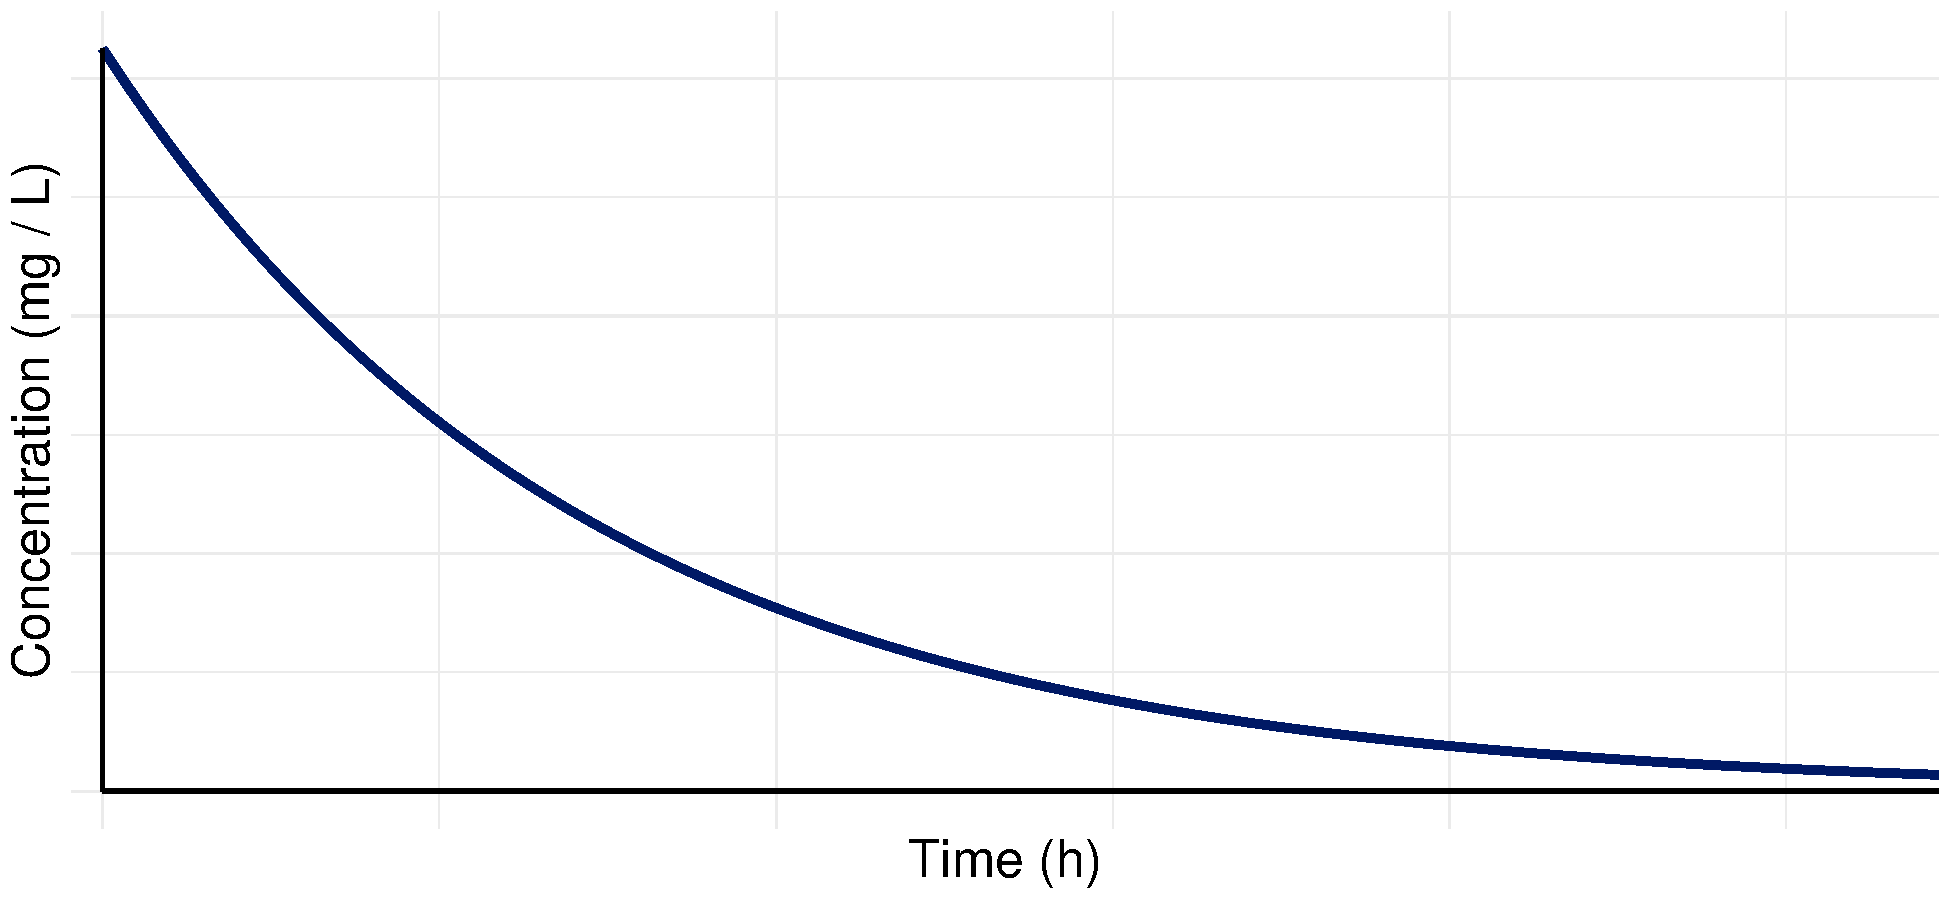
\includegraphics[width=\linewidth]{fig/img/Exposure and Css/Concentration W. IV.pdf}
        \caption{Example of drug concentration for a one-compartment model without depot.}
        \label{fig: Drug Concentration IV}
    \end{minipage}%
    \hfill
    \begin{minipage}{0.45\textwidth}
        \centering
        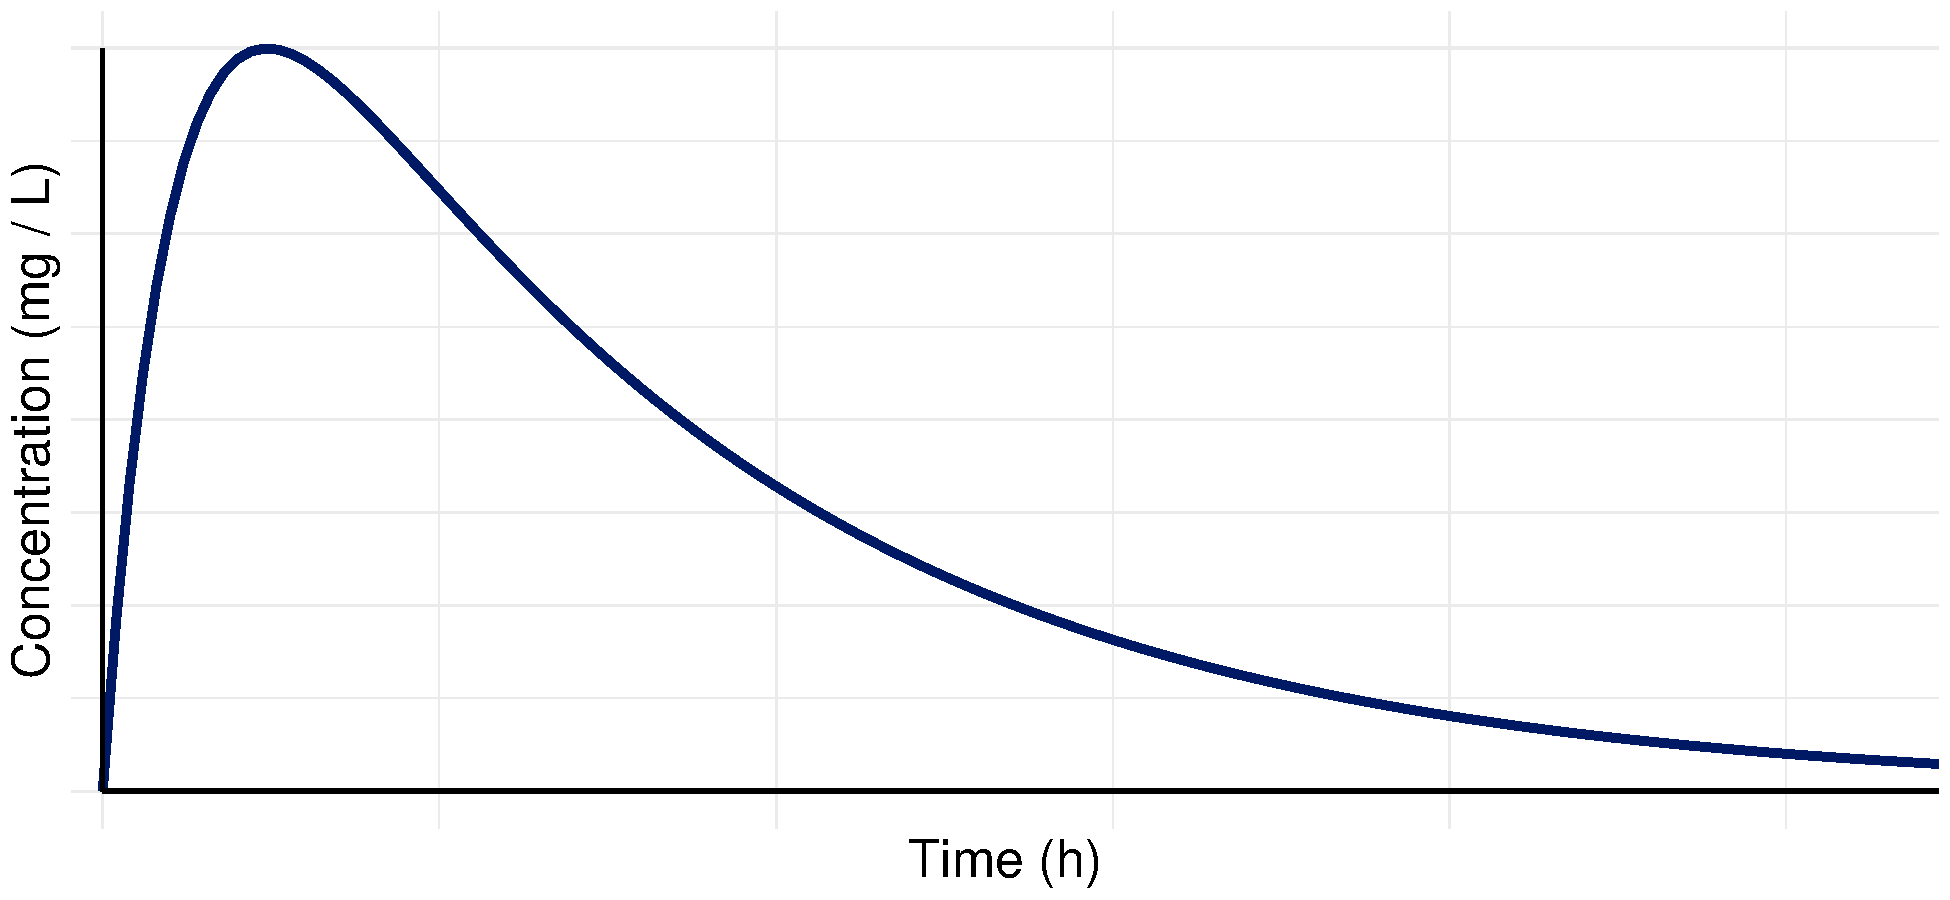
\includegraphics[width=\linewidth]{fig/img/Exposure and Css/Concentration W. Oral.pdf}
        \caption{Example of drug concentration for a one-compartment model with depot.}
        \label{fig: Drug concentration EV}
    \end{minipage}
    \label{fig: Drug concentrations}
\end{figure}

In the one-compartment model with depot (ref), $C(t_{\text{max}})$ occurs at
\begin{align} \label{eq: t_max for one com with absorption}
    t_{\text{max}} = \frac{1}{K_a - K_e} \ln\left(\frac{K_a}{K_e}\right),
\end{align}
and is obtained by setting \eqref{eq: first order kinetic of amount in central com with abs com} equal to zero and solving for $t$, see Figure \ref{fig: Drug concentration EV}. The maximum concentration is then \eqref{eq: sol to first order kinetic of amount in central com with abs com} evaluated in $t_{\text{max}}$.


%%% half-life 
The biological half-life of a drug is the time required for the concentration of a drug in the body to reduce by half. It is given by 
\begin{align}
    t_{1/2} = \frac{\ln(2)}{K_e},
\end{align}
which shows that the half-life only depends on the elimination rate constant $K_e$, meaning it remains constant regardless of the drug concentration. The half-life is obtained by setting \eqref{eq: sol to first order kinetic of amount in one com without abs} equal to $\frac{1}{2}D$ and solve for $t$. 




\section{Other dosage regiments}
\label{app: other dosage regimen}
Consider a one-compartment model with IV administration with constant rate infusion $R_{in}$ (measured in mass per time, e.g. $mg/h$), meaning that a constant amount of drug is injected per unit time. Assuming the rate of infusion is constant, and the drug elimination follows first order kinetics, the mass balance equation for the central compartment during the time of infusion is given by
\begin{align} \label{eq: Constant infusion rate}
    \Dif{A_{central}(t)}=R_{in}-K_e*A_{central}(t), 
\end{align}
where $R_{in}$ is a constant indicating the amount of drug injected into the central compartment per unit time. When the infusion of drug stops, i.e. $R_{in}=0$, the mass balance equation simply describes drug elimination following first order kinetics. The solution to \eqref{eq: Constant infusion rate} is divided by $V_d$ to obtain the solution expressed in terms of concentration,
\begin{align*}
    C_{central}(t) = \frac{R_{in}}{Cl}\left(1-\exp\left(-K_e * t\right)\right).
\end{align*}

Figure \ref{fig: IN and MD} shows an example of concentration of a drug administered IV with constant rate infusion. This illustrates that the concentration increases until the elimination rate equals the infusion rate, and a steady state is reached. This occurs as the infusion rate is constant, and the elimination rate is proportional to the drug concentration. The concentration at which steady state occurs is obtained by setting \eqref{eq: Constant infusion rate} equal to zero and using the relations \eqref{eq: Concentration} and \eqref{eq: elimination rate constant},
\begin{align*}
    R_{in} = K_e * A_{central}(t_{ss}) \Longrightarrow R_{in} = \frac{Cl}{V_d}A_{central}(t_{ss}) \Longrightarrow
    C(t_{ss}) = \frac{R_{in}}{Cl},
\end{align*}
where $C(t_{ss})$ denotes the steady state concentration at time $t_{ss}$, where $t_{ss}$ denotes time points for which \eqref{eq: Constant infusion rate} equals $0$. This implies that the steady state concentration is known given the constant infusion rate and clearance.

%%% Multiple dosing
Consider a one-compartment model with EV administration and $N$ doses given at the same time interval $\tau$ between every dose. This scenario has same method of administration and number of compartments as the scenario for the mass balance equation \eqref{eq: first order kinetic of amount in central com with abs com}, but the dosing regimen is different. Assuming the absorption follows first order kinetics, the concentration for multiple dosing is the sum of the remaining concentration of each EV administered dose received, 
\begin{align*}
    C(t) = \sum^{N-1}_{n=0} C_{single}(t-n*\tau),
\end{align*}
where $C_{single}$ is \eqref{eq: sol to first order kinetic of amount in central com with abs com} divided by $V_d$.

Multiple dosing can be interpreted as an approximation of constant rate infusion, where the administration is EV instead of IV, as IV administration is not always possible. The multiple dosing is related to the infusion rate by
\begin{align*}
    R_{in} = \frac{F * D}{\tau}.
\end{align*}

An example of concentration of a drug administered EV with multiple dosing can be seen in Figure \ref{fig: IN and MD}.
\begin{figure}[H]
    \centering
    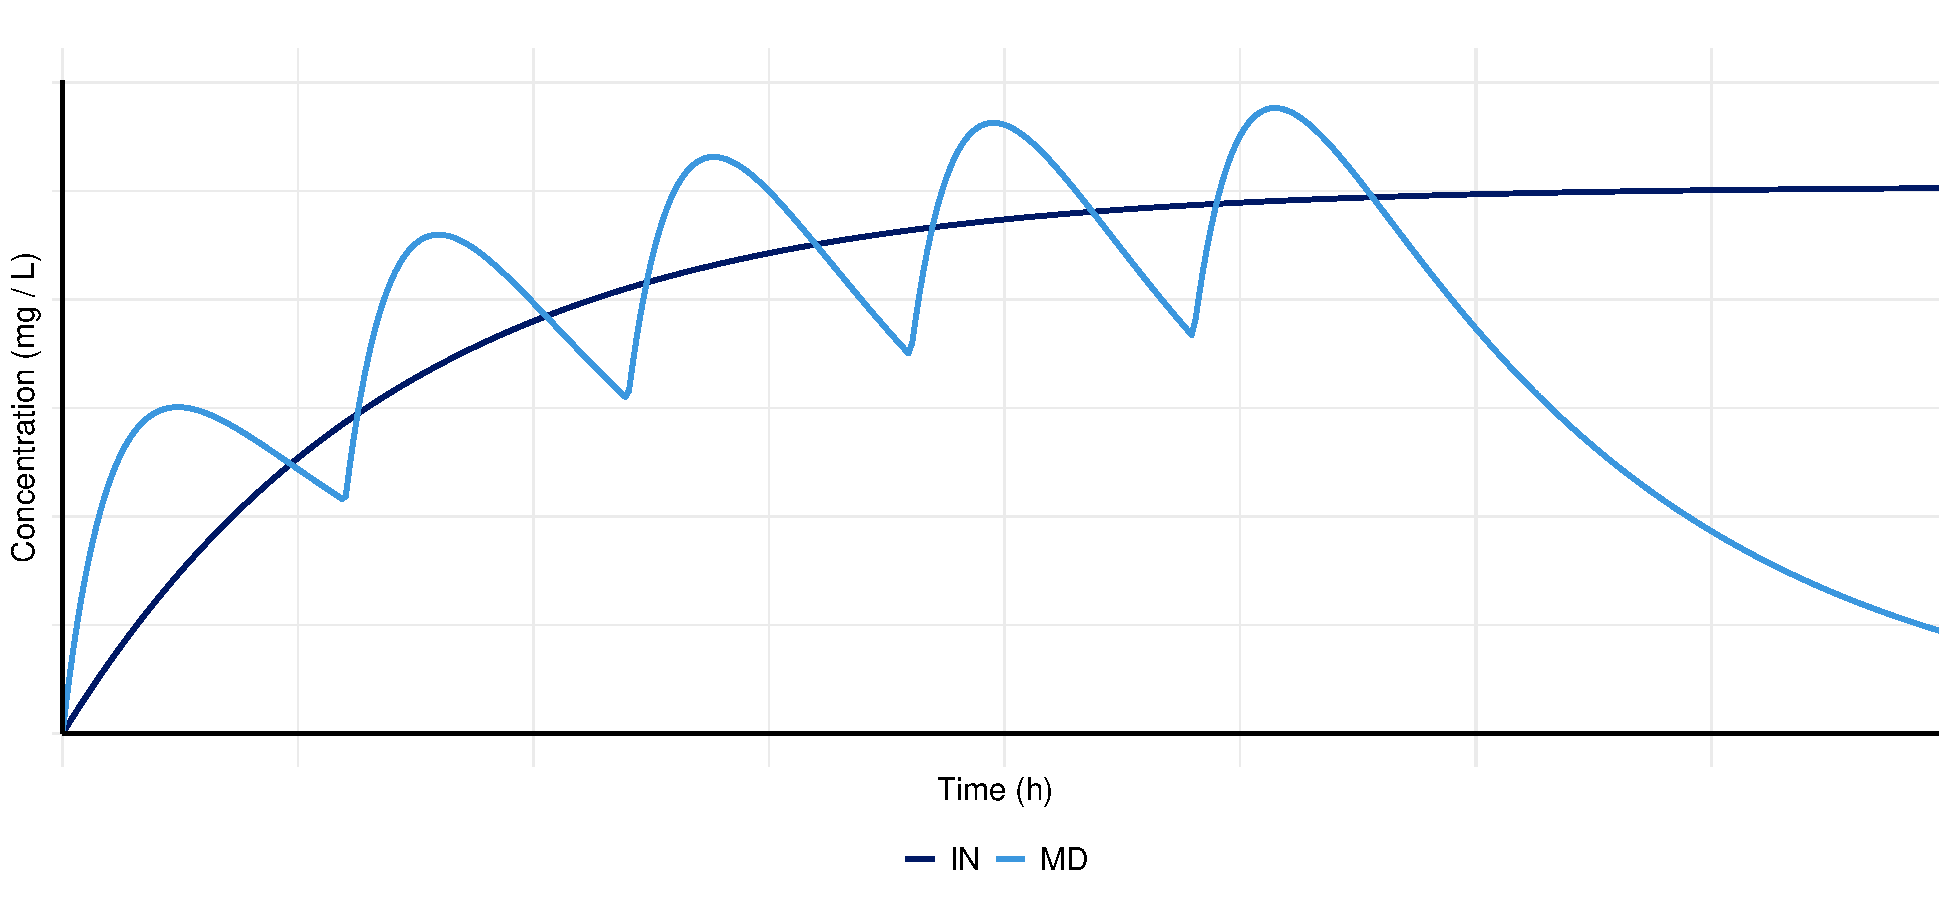
\includegraphics[width=0.9\linewidth]{fig/img/Exposure and Css/3hoursDosing.pdf}
    \caption{Example of drug concentration obtained with constant rate infusion and multiple dosing.}
    \label{fig: IN and MD}
\end{figure}



\section{Effect derivations}


The expression is obtained by 
From \eqref{eq: steady state PD}, it can be derived that
\begin{align} \label{eq: Steady state derivation}
    \frac{[R][M]}{[MR]} = K_d \implies \frac{[MR]}{R_{tot}} = \frac{[M]}{[M] + K_d},
\end{align}
where $k_d = \frac{k_{-1}}{k_1}$ is the disassociation constant.
The first equation in \eqref{eq: Steady state derivation} is obtained directly from \eqref{eq: steady state PD}, and the second equation in \eqref{eq: Steady state derivation} is derived by substituting $[R]$ in the first equation with $([R_{tot}] - [MR])$. 

To derive the expression in \eqref{eq: Steady state derivation} in terms of effect, the quantities $[MR]$ and $[R_{tot}]$ are substituted with the relationships established in \eqref{eq: effect formalisation} and \eqref{eq: effect formalisation2}, such that
\begin{align} \label{eq: Effect and concentration}
    \frac{E/\varphi}{E_{\text{max}}/\varphi} = \frac{[M]}{[M] + K_d} \implies E = \frac{E_{\text{max}}[M]}{[M] + K_d}.
\end{align}
The amount of unbounded drug molecules, $[M]$, is interpreted as the drug's concentration.


\section{Table of parameters}

\begin{table}[h!]
    \centering
    \renewcommand{\arraystretch}{1.5}
    \begin{tabular}{|p{3.4cm}|p{1.4 cm}|p{8.8cm}|}
        \hline
        \textbf{Parameter} & \textbf{Unit} & \textbf{Description} \\
        \hline
        $F$ (bioavailability) & unitless & The fraction of the administered dose that reaches the systemic circulation. \\
        \hline
        $V$ (volume of distribution) & $\text{volume}$ & Relation between total amount of drug in the body and the plasma concentration of the drug. \\
        \hline
        $Cl$ (clearance) & $\tfrac{\text{volume}}{\text{time}}$ & The volume of plasma cleared of drug per time. \\
        \hline
        $k_a$ (absorption rate constant) & $\text{time}^{-1}$ & The rate at which the drug moves from the site of administration into the systemic circulation. \\
        \hline
        $k_e$ (elimination rate constant) & $\text{time}^{-1}$ & The rate at which a drug is eliminated from the body.\\
        \hline
        $k_{12}$, $k_{21}$ (exchange rate constants) & $\text{time}^{-1}$ & The rate at which the drug distributes between various tissues of the body. \\
        \hline
    \end{tabular}
    \caption{Description of PK parameters with units of measure.}
    \label{tab: pharmacokinetic parameters summary}
\end{table}
  % \include{incl/app/appendix2}
  % ..
\end{appendices}

% The backmatter is for extra stuff. Headings are not numbered.
\backmatter

% Automatic list of references, based on which references in the literature
% database files were referenced throughout the document.
\bibliographystyle{apalike}
\bibliography{
  incl/bib/books,
  incl/bib/articles,
  incl/bib/software
}\label{bib}

\addcontentsline{toc}{chapter}{Bibliography}


\end{document}
